
%===== main document class =====
%\ifdefined\slideModeHandout
\documentclass%
[%
  handout,          % avoid unnecessary overlays
  aspectratio=169,  % aspect ratio fo 16:9 
  t,                % place content at top of frames
  10pt,             % use 10pt as standard font size (default size is 11pt)
  compress,         % compress things like navigation bars...
]{beamer}
%\else
%\documentclass%
%[%
%  aspectratio=169,  % aspect ratio fo 16:9 
%  t,                % place content at top of frames
%  10pt,             % use 10pt as standard font size (default size is 11pt)
%  compress,         % compress things like navigation bars...
%]{beamer}
%\fi

\mode<presentation>
%===============tabto==============
% tabto.sty
%
% version 1.4  (Dec 2018)
%
% Tabbing to fixed positions in a paragraph.
%
% Copyright 2006,2009,2012,2013,2018 by 
% Donald Arseneau,   Vancouver, Canada (asnd@triumf.ca)
% Permission to use, distribute and modify this software is granted
% under the conditions of the LaTeX Project Public License, either 
% version 1.3 or (at your option) any later version.  The license is
% found at http://www.latex-project.org/lppl.txt, and is part of all 
% recent distributions of LaTeX.
%
% This work has the LPPL maintenance status `maintained' (by author).
%
% Two new text positioning commands are defined: \tabto and \tab.
% 
% \tabto{<length>}
% Tab to a position relative to the left margin in a paragraph (any
% indentation due to a list or \leftskip is part of the `margin' in
% this context). If the text on the line already goes past the desired
% position, the tab starts a new line and moves to the requested
% horizontal position.
%
% \tabto*{<length>}
% Similar to \tabto, except it will perform backspacing, and over-
% print previous text on the line whenever that text is already
% longer than the specified length (i.e., no linebreak is produced).
% Line-breaks are suppressed immediately after \tabto or \tabto*.
%
% The length register "\CurrentLineWidth" will report the width
% of the existing text on the line, and it may be used in the
% <length> argument (using calc.sty, for example). Also, there
% is "\TabPrevPos" which gives the "\CurrentLineWidth" from the
% previous tab command (the position where the tab command occurred,
% not where it went to), and can be used to return to that position
% if no line breaks have occurred in between, or directly below it,
% if there were line breaks.
%
% \tab
% Tab to the next tab-stop chosen from a list of tab positions, in
% the traditional style of typewriters.  A \tab will always move
% to the next tab stop (or the next line), even if it is already
% exactly at a tab stop. Thus, "\tab" at the beginning of a line,
% or "\tab\tab" elsewhere skips a position. A linebreak is permitted 
% immediately following a \tab, in case the ensuing text does not 
% fit well in the remaining space.
%
% If you do not want to skip positions, use "\tabto{\NextTabStop}"
% instead of "\tab".  This is particularly useful when you want to
% use \tab in some other command, but do not want to skip a column
% for the first item.
%
% The tab-stop positions are declared using either \TabPositions
% or \NumTabs:
%
% \TabPositions{<length>, <length>,...<length>}
% Declares the tab stops as a comma-separated list of positions 
% relative to the left margin. A tab-stop at 0pt is implicit, and 
% need not be listed.
%
% \NumTabs{<number>}
% Declares a list of <number> equally-spaced tabs, starting at the
% left margin and spanning \linewidth.  For example \NumTabs{2} 
% declares tab-stops at 0pt and 0.5\linewidth, the same as
% \TabPositions{0pt, 0.5\linewidth} or \TabPositions{0.5\linewidth}
%
% After these declarations, the list of tab positions is saved in
% \TabStopList, and the next tab position, relative to the current 
% position, is given by \NextTabStop.  You do not normally need
% to access them, but they are available.
%
% Problems:
%
% Tall objects after a tab stop may overlap the line above, rather
% than forcing a greater separation between lines.

%\ProvidesPackage{tabto}[2018/12/28 \space v 1.4 \space 
%  Another tabbing mechanism]\relax

%%%%%%%%%Code Begin

%\newdimen\CurrentLineWidth
%\newdimen\TabPrevPos
%
%\newcommand\tabto[1]{%
% \leavevmode
% \begingroup
% \def\@tempa{*}\def\@tempb{#1}%
% \ifx\@tempa\@tempb % \tab* 
%   \endgroup
%   \TTo@overlaptrue % ... set a flag and re-issue \tabto to get argument
%   \expandafter\tabto
% \else
%   \ifinner % in a \hbox, so ignore
%   \else % unrestricted horizontal mode
%     \null% \predisplaysize will tell the position of this box (must be box)
%     \parfillskip\fill
%     \everydisplay{}\everymath{}%
%     \predisplaypenalty\@M \postdisplaypenalty\@M
%     $$% math display so we can test \predisplaysize
%      \lineskiplimit=-999pt % so we get pure \baselineskip
%      \abovedisplayskip=-\baselineskip \abovedisplayshortskip=-\baselineskip
%      \belowdisplayskip\z@skip \belowdisplayshortskip\z@skip
%      \halign{##\cr\noalign{%
%        % get the width of the line above
%        \ifdim\predisplaysize=\maxdimen %\message{Mixed R and L, so say the line is full. }%
%           \CurrentLineWidth\linewidth
%        \else
%           \ifdim\predisplaysize=-\maxdimen 
%             % \message{Not in a paragraph, so call the line empty. }%
%             \CurrentLineWidth\z@
%           \else
%             \ifnum\TTo@Direction<\z@
%               \CurrentLineWidth\linewidth \advance\CurrentLineWidth\predisplaysize
%             \else
%               \CurrentLineWidth\predisplaysize 
%             \fi
%             % Correct the 2em offset
%             \advance\CurrentLineWidth -2em
%             \advance\CurrentLineWidth -\displayindent
%             \advance\CurrentLineWidth -\leftskip
%        \fi\fi
%        \ifdim\CurrentLineWidth<\z@ \CurrentLineWidth\z@\fi
%        % Enshrine the tab-to position; #1 might reference \CurrentLineWidth
%        \setlength\@tempdimb{#1}% allow calc.sty
%        %\message{*** Tab to \the\@tempdimb, previous width is \the\CurrentLineWidth. ***}%
%        % Save width for possible return use
%        \global\TabPrevPos\CurrentLineWidth
%        % Build the action to perform
%        \protected@xdef\TTo@action{%
%           \vrule\@width\z@\@depth\the\prevdepth
%           \ifdim\CurrentLineWidth>\@tempdimb
%              \ifTTo@overlap\else
%                 \protect\newline \protect\null
%           \fi\fi
%           \protect\nobreak
%           \protect\hskip\the\@tempdimb\relax
%        }%
%        %\message{\string\TTo@action: \meaning \TTo@action. }%
%        % get back to the baseline, regardless of its depth.
%        \vskip-\prevdepth
%        \prevdepth-99\p@
%        \vskip\prevdepth
%      }}%
%      $$
%     % Don't count the display as lines in the paragraph
%     \count@\prevgraf \advance\count@-4 \prevgraf\count@
%     \TTo@action
%     %%   \penalty\@m % to allow a penalized line break
%   \fi
%   \endgroup
%   \TTo@overlapfalse
%   \ignorespaces
% \fi
%}
%
%% \tab -- to the next position
%% \hskip so \tab\tab moves two positions
%% Allow a (penalized but flexible) line-break right after the tab.
%%
%\newcommand\tab{\leavevmode\hskip2sp\tabto{\NextTabStop}%
%  \nobreak\hskip\z@\@plus 30\p@\penalty4000\hskip\z@\@plus-30\p@\relax}
%
%
%% Expandable macro to select the next tab position from the list
%
%\newcommand\NextTabStop{%
%  \expandafter \TTo@nexttabstop \TabStopList,\maxdimen,>%
%}
%
%\def\TTo@nexttabstop #1,{%
%    \ifdim#1<\CurrentLineWidth
%      \expandafter\TTo@nexttabstop
%    \else
%      \ifdim#1<0.9999\linewidth#1\else\z@\fi
%      \expandafter\strip@prefix
%    \fi
%}
%\def\TTo@foundtabstop#1>{}
%
%\newcommand\TabPositions[1]{\def\TabStopList{\z@,#1}}
%
%\newcommand\NumTabs[1]{%
%   \def\TabStopList{}%
%   \@tempdimb\linewidth 
%   \divide\@tempdimb by#1\relax
%   \advance\@tempdimb 1sp % counteract rounding-down by \divide
%   \CurrentLineWidth\z@
%   \@whiledim\CurrentLineWidth<\linewidth\do {%
%     \edef\TabStopList{\TabStopList\the\CurrentLineWidth,}%
%     \advance\CurrentLineWidth\@tempdimb
%   }%
%   \edef\TabStopList{\TabStopList\linewidth}%
%}
%
% %default setting of tab positions:
%\TabPositions{\parindent,.5\linewidth}
%
%%\newif\ifTTo@overlap \TTo@overlapfalse
%
%%\@ifundefined{predisplaydirection}{
%% \let\TTo@Direction\predisplaysize
%% \let\predisplaydirection\@undefined
%%}{
%% \let\TTo@Direction\predisplaydirection
%%}
%
%

% ===== include packages =====
\usepackage{lmodern}
\usepackage[utf8]{inputenc}      % Unicode UTF-8 encoding support
\usepackage[T2A,T1]{fontenc}         % T1 font encoding
\usepackage{etoolbox}            % Programming tools (used for \insertpartstartframe, \insertpartendframe)
\usepackage{ifthen}              % Simple conditional statements
\usepackage{amsmath}             % AMS math package
\usepackage{amssymb}             % Extended collection of math symbols
\usepackage{mathtools}           % More math stuff
\usepackage{nicefrac}            % Nice fractions
\usepackage{xcolor}              % Driver independent colors
\usepackage{colortbl}            % rowcolor for tables
\usepackage{array}               % tables and arrays with extended features (e.g., overlays)
\usepackage{makecell}            % Simple formatting of single table cells
\usepackage{multirow}            % Multi-rows in tabular environments
\usepackage{booktabs}            % More flexible lines for tabular environments
\usepackage{tabto}               % Easy way of specifying tabulators
\usepackage{adjustbox}           % Macros for adjusting boxed content (used in defining \fitbox)
\usepackage{relsize}             % Relative font sizes (\larger=\relsize{1}, \smaller=\relsize{-1})
\usepackage{graphicx}            % Inserting pictures
\usepackage{hyperref}            % Cross referencing
%\usepackage{media9}              % Include media objects
%\usepackage{animate}             % Animations
\usepackage{tikz}                % TikZ library for drawing
\usepackage{pgfplots}            % Plots
\usepackage{import}              % including stuff with relative paths
%\usepackage{listings}            % source code inclusion

%===== TikZ libraries =====
\usetikzlibrary{shapes}          % Additional shapes: Ellipse
\usetikzlibrary{shapes.symbols}  % Additional shapes: Symbols (e.g., "cloud")
\usetikzlibrary{shapes.arrows}   % Additional shapes: Arrows (e.g., "single arrow")
\usetikzlibrary{arrows}          % Arrow tips
\usetikzlibrary{arrows.meta}     % Adjustable arrow heads
\usetikzlibrary{positioning}     % Relative positioning of nodes

%===== pgfsetting =====
\pgfplotsset{compat=newest}      % Use newest version of pgf
\usepgfplotslibrary{fillbetween} % filling between curves

%===== nice tables =====
\setlength{\heavyrulewidth}{0.08em}
\setlength{\lightrulewidth}{0.08em}
\setlength{\cmidrulewidth}{0.04em}
\setlength{\aboverulesep}{0.4ex}
\setlength{\belowrulesep}{0.6ex}
\newcommand{\cmidbeg}{\addlinespace[0.40ex]}
\newcommand{\cmidend}{\addlinespace[0.10ex]}

\usepackage{caption}
\usepackage{subcaption}


%%%%%%%%%%%%%%%%%%%%%%%%%%%%%%%%%%%%%%%%%%%%%%%%%%%%%%%%%%%%
%%%%%%
%%%%%%     M A I N   D O C U M E N T   S W I T C H E S     
%%%%%%
%%%%%%%%%%%%%%%%%%%%%%%%%%%%%%%%%%%%%%%%%%%%%%%%%%%%%%%%%%%%

% define command for directly using switches
\newcommand{\usetoggle}[1]{\iftoggle{#1}{true}{false}}

% define switches
\newtoggle{useNavSymbols}               % display of navigation symbols
\newtoggle{useShadows}                  % use blocks with shadows
\newtoggle{useColorBlocks}              % use colored blocks
\newtoggle{useColorBlockTitles}         % use colored block titles
\newtoggle{useInverseBlockTitles}       % use colored block title background with white text
\newtoggle{altColors}                   % use alternative color theme
\newtoggle{addExercises}                % whether exercises are used
\newtoggle{specialHeiko}                % special stuff for Heiko
\newtoggle{specialThomas}               % special stuff for Thomas

\def\slideStyleThomas{..}


\ifdefined\slideStyleThomas

  %>>>>>>>>>> parameters for Thomas >>>>>>>>>>
  \title%
      [Image and Video Coding]%
      {Image and Video Coding I:\\[0.5ex] Fundamentals}
  \author%
      [T. Wiegand, J. Pfaff, J. Rasch]%
      {Thomas Wiegand, Jonathan Pfaff, Jennifer Rasch}
  \institute%
      [TU Berlin, Fraunhofer HHI]%
      {Technische Universität Berlin, Fraunhofer Heinrich Hertz Institute, Berlin}

  \newcommand{\slideOrganization}{}

  \settoggle{useNavSymbols}        {false}
  \settoggle{useShadows}           {true}
  \settoggle{useColorBlocks}       {true}
  \settoggle{useColorBlockTitles}  {true}
  \settoggle{useInverseBlockTitles}{true}
  \settoggle{altColors}            {false}
  \settoggle{addExercises}         {false}

  \settoggle{specialHeiko}         {false}
  \settoggle{specialThomas}        {true}
  %<<<<<<<<<< parameters for Thomas <<<<<<<<<<

\else

  %>>>>>>>>>> parameters for Heiko >>>>>>>>>>
  \title%
      {Data Compression}
  \author%
      [Heiko Schwarz]%
      {Heiko Schwarz}
  \institute%
      [Freie Universität Berlin]%
      {Freie Universität Berlin\\%
      Fachbereich Mathematik und Informatik}

\ifdefined\slideModeHandout
  \settoggle{useNavSymbols}        {false}
\else
  \settoggle{useNavSymbols}        {false}
\fi
  \settoggle{useShadows}           {true}
  \settoggle{useColorBlocks}       {true}
  \settoggle{useColorBlockTitles}  {true}
  \settoggle{useInverseBlockTitles}{true}
  \settoggle{altColors}            {false}
  \settoggle{addExercises}         {true}

  \settoggle{specialHeiko}         {true}
  \settoggle{specialThomas}        {false}
  %<<<<<<<<<< parameters for Heiko <<<<<<<<<<

\fi % end of conditional





%%%%%%%%%%%%%%%%%%%%%%%%%%%%%%%%%%%%%%%%%%%%%%%%%
%%%%%%
%%%%%%     C U S T O M I Z E   D E S I G N
%%%%%%
%%%%%%%%%%%%%%%%%%%%%%%%%%%%%%%%%%%%%%%%%%%%%%%%%

%===== spacing for lists and paragraphs (modified copy from beamerbaselocalstructure.sty) =====
\makeatletter
\setlength  \parskip         {2ex}
\setlength  \leftmargini     {2em}
\setlength  \leftmarginii    {2em}
\setlength  \leftmarginiii   {2em}
\setlength  \labelsep        {.5em}
\setlength  \labelwidth      {\leftmargini}
\addtolength\labelwidth      {-\labelsep}
\def\@listi  {\leftmargin\leftmargini
              \partopsep  \parskip
              \parskip    0.0\p@
              \parsep     0.0\p@
              \topsep     3.0\p@ \@plus1.0\p@ \@minus2.0\p@
              \itemsep    3.0\p@ \@plus1.0\p@ \@minus2.0\p@}
\let\@listI\@listi
\def\@listii {\leftmargin\leftmarginii
              \parsep     0.0\p@
              \topsep     3.0\p@ \@plus1.0\p@ \@minus2.0\p@
              \itemsep    3.0\p@ \@plus1.0\p@ \@minus2.0\p@}
\def\@listiii{\leftmargin\leftmarginiii
              \parsep     0.0\p@
              \topsep     3.0\p@ \@plus1.0\p@ \@minus2.0\p@
              \itemsep    3.0\p@ \@plus1.0\p@ \@minus2.0\p@}
\makeatother


%===== counter for exercises =====
\newcounter{exercise}


%===== enumerate symbols (modified copy from beamerbaseauxtemplates.sty) =====
\makeatletter

%--- define commands for changing enum style ---
\newcommand{\setenumstyledepth}[2]{% {enumdepth}{command for displaying counter}
  \ifthenelse{\equal{#1}{1}}%
     {\renewcommand*{\theenumi}{#2{enumi}}}%
     {\ifthenelse{\equal{#1}{2}}%
        {\renewcommand*{\theenumii}{#2{enumii}}}%
        {\renewcommand*{\theenumiii}{#2{enumiii}}}%
     }%
}
% Note: For the following command you can also use your own styles.
%       For example, a style "A." in a smaller font can be defined by
%         \newcommand{\AlphaDot}[1]{{\smaller\smaller\Alph{#1}.}}
\newcommand{\enumStyle}[1]{\setenumstyledepth{\the\@enumdepth}{#1}}
\newcommand{\enumStylesDefault}[3]{%
  \setenumstyledepth{1}{#1}%
  \setenumstyledepth{2}{#2}%
  \setenumstyledepth{3}{#3}%
}

%--- define commands for putting enum symbols ---
\newcommand{\putenumsquare}[1]{%
  \smaller%
  \usebeamercolor[bg]{\beameritemnestingprefix item projected}%
  \begin{pgfpicture}{-1ex}{-0.25ex}{1.1ex}{2.0ex}%
    \pgfpathrectangle{\pgfpoint{-1.2ex}{-0.6ex}}{\pgfpoint{2.4ex}{2.4ex}}%
    \pgfusepath{fill}%
    \pgftext[base,y=-0.15ex]{\color{fg}#1}%
  \end{pgfpicture}%
}
\newcommand{\putenumcircle}[1]{%
  \smaller%
  \usebeamercolor[bg]{\beameritemnestingprefix item projected}%
  \begin{pgfpicture}{-1ex}{-0.25ex}{1.1ex}{2.0ex}%
    \pgfpathcircle{\pgfpoint{0pt}{.6ex}}{1.3ex}%
    \pgfusepath{fill}%
    \pgftext[base,y=-0.15ex]{\color{fg}#1}%
  \end{pgfpicture}%
}
\newcommand{\putenumblank}[1]{%
  \smaller%
  \begin{pgfpicture}{-1ex}{-0.25ex}{1.1ex}{2.0ex}%
    \pgfpathrectangle{\pgfpoint{-1.2ex}{-0.6ex}}{\pgfpoint{2.4ex}{2.4ex}}%
    \pgftext[base,y=-0.15ex]{#1}%
  \end{pgfpicture}%
}
\newcommand{\putenumbracket}[1]{%
  \smaller%
  \begin{pgfpicture}{-1ex}{-0.25ex}{1.1ex}{2.0ex}%
    \pgfpathrectangle{\pgfpoint{-1.2ex}{-0.6ex}}{\pgfpoint{2.4ex}{2.4ex}}%
    \pgftext[base,y=-0.15ex]{$\boldsymbol{\langle}$#1$\boldsymbol{\rangle}$}%
  \end{pgfpicture}%
}
\newcommand{\putenumautoi}[1]{\putenumcircle{#1}}
\newcommand{\putenumautoii}[1]{\putenumcircle{#1}}
\newcommand{\putenumautoiii}[1]{\putenumcircle{#1}}
\newcommand{\putenumauto}[1]{%
  \ifthenelse{\equal{\the\@itemdepth}{1}}%
     {\putenumautoi{#1}}%
     {\ifthenelse{\equal{\the\@itemdepth}{2}}%
        {\putenumautoii{#1}}%
        {\putenumautoiii{#1}}%
     }%
}

%--- define beamer enum templates [square][circle][blank][bracket][auto] ---
\expandafter\let\csname beamer@@tmpop@enumerate item@square\endcsname\relax
\expandafter\let\csname beamer@@tmpop@enumerate subitem@square\endcsname\relax
\expandafter\let\csname beamer@@tmpop@enumerate subsubitem@square\endcsname\relax
\expandafter\let\csname beamer@@tmpop@enumerate mini template@square\endcsname\relax

\expandafter\let\csname beamer@@tmpop@enumerate item@circle\endcsname\relax
\expandafter\let\csname beamer@@tmpop@enumerate subitem@circle\endcsname\relax
\expandafter\let\csname beamer@@tmpop@enumerate subsubitem@circle\endcsname\relax
\expandafter\let\csname beamer@@tmpop@enumerate mini template@circle\endcsname\relax

\defbeamertemplate{enumerate item}{square}{\putenumsquare{\insertenumlabel}}
\defbeamertemplate{enumerate subitem}{square}{\putenumsquare{\insertsubenumlabel}}
\defbeamertemplate{enumerate subsubitem}{square}{\putenumsquare{\insertsubsubenumlabel}}
\defbeamertemplate{enumerate mini template}{square}{\putenumsquare{\insertenumlabel}}

\defbeamertemplate{enumerate item}{circle}{\putenumcircle{\insertenumlabel}}
\defbeamertemplate{enumerate subitem}{circle}{\putenumcircle{\insertsubenumlabel}}
\defbeamertemplate{enumerate subsubitem}{circle}{\putenumcircle{\insertsubsubenumlabel}}
\defbeamertemplate{enumerate mini template}{circle}{\putenumcircle{\insertenumlabel}}

\defbeamertemplate{enumerate item}{blank}{\putenumblank{\insertenumlabel}}
\defbeamertemplate{enumerate subitem}{blank}{\putenumblank{\insertsubenumlabel}}
\defbeamertemplate{enumerate subsubitem}{blank}{\putenumblank{\insertsubsubenumlabel}}
\defbeamertemplate{enumerate mini template}{blank}{\putenumblank{\insertenumlabel}}

\defbeamertemplate{enumerate item}{bracket}{\putenumbracket{\insertenumlabel}}
\defbeamertemplate{enumerate subitem}{bracket}{\putenumbracket{\insertsubenumlabel}}
\defbeamertemplate{enumerate subsubitem}{bracket}{\putenumbracket{\insertsubsubenumlabel}}
\defbeamertemplate{enumerate mini template}{bracket}{\putenumbracket{\insertenumlabel}}

\defbeamertemplate{enumerate item}{auto}{\putenumauto{\insertenumlabel}}
\defbeamertemplate{enumerate subitem}{auto}{\putenumauto{\insertsubenumlabel}}
\defbeamertemplate{enumerate subsubitem}{auto}{\putenumauto{\insertsubsubenumlabel}}
\defbeamertemplate{enumerate mini template}{auto}{\putenumauto{\insertenumlabel}}

%--- define commands for easily changing enum modes ---
% The outcommented simple version has a problem with enum nested in itemize (wrong level)
%   \newcommand{\enumMode}[1]{\setbeamertemplate{enumerate \beameritemnestingprefix item}[#1]} 
\newcommand{\enumMode}[1]{%
  \ifthenelse{\equal{\the\@enumdepth}{1}}%
     {\setbeamertemplate{enumerate item}[#1]}%
     {\ifthenelse{\equal{\the\@enumdepth}{2}}%
        {\setbeamertemplate{enumerate subitem}[#1]}%
        {\setbeamertemplate{enumerate subsubitem}[#1]}%
     }%
}
\newcommand{\enumAutoDefault}[3]{%
  \renewcommand*{\putenumautoi}[1]{\csname putenum#1\endcsname{##1}}%
  \renewcommand*{\putenumautoii}[1]{\csname putenum#2\endcsname{##1}}%
  \renewcommand*{\putenumautoiii}[1]{\csname putenum#3\endcsname{##1}}%
}

\makeatother



%===== itemize symbols (modified copy from beamerbaseauxtemplates.sty) =====
\makeatletter

%--- new item symbols ---
\newcommand{\isquare}{%
  \begin{pgfpicture}%
    \pgfpathrectangle{\pgfpointorigin}{\pgfpoint{1.0ex}{1.0ex}}%
    \pgfusepath{fill}%
    \pgfsetbaseline{-0.2ex}%
  \end{pgfpicture}%
}
\newcommand{\icircle}{%
  \begin{pgfpicture}%
    \pgfpathcircle{\pgfpoint{0pt}{.5ex}}{0.5ex}%
    \pgfusepath{fill}%
    \pgfsetbaseline{-0.2ex}%
  \end{pgfpicture}%
}
\newcommand{\itriangle}{%
  \begin{pgfpicture}%
    \pgfpathmoveto{\pgfpointorigin}
    \pgfpathlineto{\pgfpoint{0.0ex}{1.0ex}}%
    \pgfpathlineto{\pgfpoint{1.0ex}{0.5ex}}%
    \pgfusepath{fill}%
    \pgfsetbaseline{-0.2ex}%
  \end{pgfpicture}%
}
\newcommand{\idash}{%
  \begin{pgfpicture}%
    \pgfpathrectangle{\pgfpoint{0.0ex}{0.4ex}}{\pgfpoint{1.0ex}{0.2ex}}%
    \pgfusepath{fill}%
    \pgfsetbaseline{-0.2ex}%
  \end{pgfpicture}%
}
\newcommand{\iarrow}{%
  \begin{pgfpicture}%
    \pgfpathmoveto{\pgfpointorigin}
    \pgfpathlineto{\pgfpoint{-0.80ex}{ 0.75ex}}%    (-hl)( ht)  % tl =      total length
    \pgfpathlineto{\pgfpoint{-0.80ex}{ 0.25ex}}%    (-hl)( tt)  % tt = half total thickness
    \pgfpathlineto{\pgfpoint{-2.00ex}{ 0.25ex}}%    (-tl)( tt)  % hl =      head length
    \pgfpathlineto{\pgfpoint{-2.00ex}{-0.25ex}}%    (-tl)(-tt)  % ht = half head thickness
    \pgfpathlineto{\pgfpoint{-0.80ex}{-0.25ex}}%    (-hl)(-tt)
    \pgfpathlineto{\pgfpoint{-0.80ex}{-0.75ex}}%    (-hl)(-ht)
    \pgfusepath{fill}%
  \end{pgfpicture}%
}
\newcommand{\idarrow}{%
  \begin{pgfpicture}%
    \pgfpathmoveto{\pgfpointorigin}
    \pgfpathlineto{\pgfpoint{-0.80ex}{ 0.75ex}}%    (-hl)( ht)  % tl =      total length
    \pgfpathlineto{\pgfpoint{-0.80ex}{ 0.25ex}}%    (-hl)( tt)  % tt = half total thickness
    \pgfpathlineto{\pgfpoint{-2.00ex}{ 0.25ex}}%    (-tl)( tt)  % hl =      head length
    \pgfpathlineto{\pgfpoint{-2.00ex}{ 0.75ex}}%
    \pgfpathlineto{\pgfpoint{-2.80ex}{ 0.00ex}}%
    \pgfpathlineto{\pgfpoint{-2.00ex}{-0.75ex}}%
    \pgfpathlineto{\pgfpoint{-2.00ex}{-0.25ex}}%    (-tl)(-tt)  % ht = half head thickness
    \pgfpathlineto{\pgfpoint{-0.80ex}{-0.25ex}}%    (-hl)(-tt)
    \pgfpathlineto{\pgfpoint{-0.80ex}{-0.75ex}}%    (-hl)(-ht)
    \pgfusepath{fill}%
  \end{pgfpicture}%
}

%--- define beamer item templates [square][circle][triangle][dash][arrow] ---
\expandafter\let\csname beamer@@tmpop@itemize item@square\endcsname\relax
\expandafter\let\csname beamer@@tmpop@itemize subitem@square\endcsname\relax
\expandafter\let\csname beamer@@tmpop@itemize subsubitem@square\endcsname\relax

\expandafter\let\csname beamer@@tmpop@itemize item@circle\endcsname\relax
\expandafter\let\csname beamer@@tmpop@itemize subitem@circle\endcsname\relax
\expandafter\let\csname beamer@@tmpop@itemize subsubitem@circle\endcsname\relax

\expandafter\let\csname beamer@@tmpop@itemize item@triangle\endcsname\relax
\expandafter\let\csname beamer@@tmpop@itemize subitem@triangle\endcsname\relax
\expandafter\let\csname beamer@@tmpop@itemize subsubitem@triangle\endcsname\relax

\defbeamertemplate{itemize item}{square}{\isquare}
\defbeamertemplate{itemize subitem}{square}{\isquare}
\defbeamertemplate{itemize subsubitem}{square}{\isquare}

\defbeamertemplate{itemize item}{circle}{\icircle}
\defbeamertemplate{itemize subitem}{circle}{\icircle}
\defbeamertemplate{itemize subsubitem}{circle}{\icircle}

\defbeamertemplate{itemize item}{triangle}{\itriangle}
\defbeamertemplate{itemize subitem}{triangle}{\itriangle}
\defbeamertemplate{itemize subsubitem}{triangle}{\itriangle}

\defbeamertemplate{itemize item}{dash}{\idash}
\defbeamertemplate{itemize subitem}{dash}{\idash}
\defbeamertemplate{itemize subsubitem}{dash}{\idash}

\defbeamertemplate{itemize item}{arrow}{\iarrow}
\defbeamertemplate{itemize subitem}{arrow}{\iarrow}
\defbeamertemplate{itemize subsubitem}{arrow}{\iarrow}

%--- define command for easily changing item styles ---
\newcommand{\itemMode}[1]{\setbeamertemplate{itemize \beameritemnestingprefix item}[#1]}

\makeatother



%===== commands for text highlighting  =====
% helping command
\newcommand{\setfontrm} {\fontshape{\rmdefault}\selectfont}
\newcommand{\setfontit} {\fontshape{\itdefault}\selectfont}
\newcommand{\setfontrs} {\fontseries{\mddefault}\selectfont}
\newcommand{\setfontbs} {\fontseries{\bfdefault}\selectfont}
\newcommand{\setfontrrm}{\fontseries{\mddefault}\fontshape{\rmdefault}\selectfont}
\newcommand{\setfontrit}{\fontseries{\mddefault}\fontshape{\itdefault}\selectfont}
\newcommand{\setfontbrm}{\fontseries{\bfdefault}\fontshape{\rmdefault}\selectfont}
\newcommand{\setfontbit}{\fontseries{\bfdefault}\fontshape{\itdefault}\selectfont}
% normal text attributes:
  % setting series
  \newcommand<>{\regu}  [1]{{\only#2{\setfontrs}#1}}
  \newcommand<>{\bold}  [1]{{\only#2{\setfontbs}#1}}
  % setting shape
  \newcommand<>{\norm}  [1]{{\only#2{\setfontrm}#1}}
  \newcommand<>{\ital}  [1]{{\only#2{\setfontit}#1}}
  % setting series and shape
  \newcommand<>{\rnorm} [1]{{\only#2{\setfontrrm}#1}}
  \newcommand<>{\rital} [1]{{\only#2{\setfontrit}#1}}
  \newcommand<>{\bnorm} [1]{{\only#2{\setfontbrm}#1}}
  \newcommand<>{\bital} [1]{{\only#2{\setfontbit}#1}}
% special text highlighting:
  % changing color only
\renewcommand<>{\alert} [1]{{\only#2{\usebeamercolor{alerted text}\color{fg}}#1}}
  \newcommand<>{\struc} [1]{{\only#2{\usebeamercolor{structure}\color{fg}}#1}}
  \newcommand<>{\examp} [1]{{\only#2{\usebeamercolor{example text}\color{fg}}#1}}
  % changing color and series
  \newcommand<>{\Alert} [1]{{\only#2{\setfontrs\usebeamercolor{alerted text}\color{fg}}#1}}
  \newcommand<>{\Struc} [1]{{\only#2{\setfontrs\usebeamercolor{structure}\color{fg}}#1}}
  \newcommand<>{\Examp} [1]{{\only#2{\setfontrs\usebeamercolor{example text}\color{fg}}#1}}
  \newcommand<>{\ALERT} [1]{{\only#2{\setfontbs\usebeamercolor{alerted text}\color{fg}}#1}}
  \newcommand<>{\STRUC} [1]{{\only#2{\setfontbs\usebeamercolor{structure}\color{fg}}#1}}
  \newcommand<>{\EXAMP} [1]{{\only#2{\setfontbs\usebeamercolor{example text}\color{fg}}#1}}
  % changing color and shape
  \newcommand<>{\ralert}[1]{{\only#2{\setfontrm\usebeamercolor{alerted text}\color{fg}}#1}}
  \newcommand<>{\rstruc}[1]{{\only#2{\setfontrm\usebeamercolor{structure}\color{fg}}#1}}
  \newcommand<>{\rexamp}[1]{{\only#2{\setfontrm\usebeamercolor{example text}\color{fg}}#1}}
  \newcommand<>{\ialert}[1]{{\only#2{\setfontit\usebeamercolor{alerted text}\color{fg}}#1}}
  \newcommand<>{\istruc}[1]{{\only#2{\setfontit\usebeamercolor{structure}\color{fg}}#1}}
  \newcommand<>{\iexamp}[1]{{\only#2{\setfontit\usebeamercolor{example text}\color{fg}}#1}}
  % changing color, shape, and series
  \newcommand<>{\rAlert}[1]{{\only#2{\setfontrrm\usebeamercolor{alerted text}\color{fg}}#1}}
  \newcommand<>{\rStruc}[1]{{\only#2{\setfontrrm\usebeamercolor{structure}\color{fg}}#1}}
  \newcommand<>{\rExamp}[1]{{\only#2{\setfontrrm\usebeamercolor{example text}\color{fg}}#1}}
  \newcommand<>{\rALERT}[1]{{\only#2{\setfontbrm\usebeamercolor{alerted text}\color{fg}}#1}}
  \newcommand<>{\rSTRUC}[1]{{\only#2{\setfontbrm\usebeamercolor{structure}\color{fg}}#1}}
  \newcommand<>{\rEXAMP}[1]{{\only#2{\setfontbrm\usebeamercolor{example text}\color{fg}}#1}}
  \newcommand<>{\iAlert}[1]{{\only#2{\setfontrit\usebeamercolor{alerted text}\color{fg}}#1}}
  \newcommand<>{\iStruc}[1]{{\only#2{\setfontrit\usebeamercolor{structure}\color{fg}}#1}}
  \newcommand<>{\iExamp}[1]{{\only#2{\setfontrit\usebeamercolor{example text}\color{fg}}#1}}
  \newcommand<>{\iALERT}[1]{{\only#2{\setfontbit\usebeamercolor{alerted text}\color{fg}}#1}}
  \newcommand<>{\iSTRUC}[1]{{\only#2{\setfontbit\usebeamercolor{structure}\color{fg}}#1}}
  \newcommand<>{\iEXAMP}[1]{{\only#2{\setfontbit\usebeamercolor{example text}\color{fg}}#1}}
% specials: Emphasizing and names [May want to redefine in actually used style]
\renewcommand<>{\emph}  [1]{\alert#2{#1}}
  \newcommand<>{\Emph}  [1]{\ALERT#2{#1}}
  \newcommand<>{\EMPH}  [1]{\iALERT#2{#1}}
  \newcommand  {\aname} [1]{{\rmfamily\scshape #1}}



%===== define subblock environments =====
\makeatletter
\newenvironment{nesting}{%
  \par\hspace{2\beamer@leftmargin}
  \begin{minipage}{\linewidth-\beamer@leftmargin-3.5\beamer@rightmargin}%
}{%
  \end{minipage}
}
\makeatother



%===== define hooks for accessing frame number inside part  =====
\makeatletter
\newcount\beamer@partstartframe
\beamer@partstartframe=1
\apptocmd{\beamer@part}{\addtocontents{nav}{\protect\headcommand{%
    \protect\beamer@partframes{\the\beamer@partstartframe}{\the\c@framenumber}}}}{}{}
\apptocmd{\beamer@part}{\beamer@partstartframe=\c@framenumber\advance\beamer@partstartframe by1\relax}{}{}
\AtEndDocument{\immediate\write\@auxout{\string\@writefile{nav}%
    {\noexpand\headcommand{\noexpand\beamer@partframes{\the\beamer@partstartframe}{\the\c@framenumber}}}}}{}{}
\def\beamer@startframeofpart{1}
\def\beamer@endframeofpart{1}
\def\beamer@partframes#1#2{%
    \ifnum\c@framenumber<#1%
    \else%
    \ifnum\c@framenumber>#2%
    \else%
    \gdef\beamer@startframeofpart{#1}%
    \gdef\beamer@endframeofpart{#2}%
    \fi%
    \fi%
}
\newcommand\insertpartstartframe{\beamer@startframeofpart}
\newcommand\insertpartendframe{\beamer@endframeofpart}
\makeatother
\def\inserttotalpartframenumber{%
    \pgfmathparse{(\insertpartendframe-\insertpartstartframe+1)}%
    \pgfmathprintnumber[fixed,precision=2]{\pgfmathresult}%
}
\def\insertpartframenumber{%
    \pgfmathparse{(\insertframenumber-\insertpartstartframe+1)}%
    \pgfmathprintnumber[fixed,precision=2]{\pgfmathresult}%
}



%===== define visible on macro for tikz pictures  =====
% see https://tex.stackexchange.com/questions/55806/mindmap-tikzpicture-in-beamer-reveal-step-by-step#55849
\tikzset{
  invisible/.style={opacity=0},
  visible on/.style={alt={#1{}{invisible}}},
  alt/.code args={<#1>#2#3}{%
    \alt<#1>{\pgfkeysalso{#2}}{\pgfkeysalso{#3}} % \pgfkeysalso doesn't change the path
  },
  action/.code args={<#1>#2}{%
    \action<#1>{\pgfkeysalso{#2}} % \pgfkeysalso doesn't change the path
  },
}
% see https://tex.stackexchange.com/questions/6135/how-to-make-beamer-overlays-with-tikz-node
\tikzset{onslide/.code args={<#1>#2}{% \pgfkeysalso doesn't change the path
  \only<#1>{\pgfkeysalso{#2}} %
}}
\tikzset{temporal/.code args={<#1>#2#3#4}{% \pgfkeysalso doesn't change the path
  \temporal<#1>{\pgfkeysalso{#2}}{\pgfkeysalso{#3}}{\pgfkeysalso{#4}} %
}}


%===== further helpful tikz macros =====
\newcommand{\budash}{{\tikz[baseline=0.1ex]\draw[thick](0,0)--({0.6em},0);}}
\newcommand{\nudash}{{\tikz[baseline=0.1ex]\draw[]     (0,0)--({0.6em},0);}}



%===== define a fitbox command  =====
\makeatletter
\newlength{\fitboxw}
\newlength{\fitboxh}
\newlength{\slideinnerheight}
\setlength{\slideinnerheight}{0.85\textheight} %%% could be reset later
\newcommand<>{\fitbox}[4][c]{%
  \only#5{%
    {%
      \setlength{\fitboxw}{#2}%
      \setlength{\fitboxh}{#3}%
      \parbox[#1][\fitboxh]{\fitboxw}{%
        \centering%
        \vfill%
        \adjustbox{%
          min width=\fitboxw,%
          min height=\fitboxh,%
          max width=\fitboxw,%
          max height=\fitboxh%
        }%
        {#4}%
        \vfill%
      }%
    }%
  }%
}
\newcommand<>{\hfitbox}[3][c]{%
  \only#4{%
    {%
      \setlength{\fitboxw}{#2}%
      \parbox[#1]{\fitboxw}{%
        \adjustbox{%
          min width=\fitboxw,%
          max width=\fitboxw}%
        {#3}%
      }%
    }%
  }%
}
\newcommand<>{\slidehfitbox}[1]{%
  \hfitbox#2{\textwidth}{#1}%
}
\newcommand<>{\slidefitbox}[1]{%
  \fitbox#2{\textwidth}{\slideinnerheight}{#1}%
}
\makeatother



%===== command for adding new part with part page / adding title page  =====
\newcommand{\startnewpart}[2][\usebeamercolor{background}\color{bg}\rule{1pt}{1pt}]{
  \part{#2}
  {
    \setbeamertemplate{navigation symbols}{}
    \begin{frame}[plain]
    \vfill\vfill
    {\hfill\begin{beamercolorbox}[%
       sep=8pt,dp=1ex,center,wd=0.8\textwidth,%
       rounded=true,
       shadow=\usetoggle{useShadows}%
    ]%
    {part title}
    \usebeamerfont{part title}\insertpart\par
    \end{beamercolorbox}\hfill}
    \vfill
    {\hfill{\fitbox{0.8\textwidth}{0.45\textheight}{#1}}\hfill}
    \vspace{0pt}
    \end{frame}
  }
}
\newcommand{\addtitlepage}{
  {
    \setbeamertemplate{navigation symbols}{}
    \begin{frame}[plain]
    \vspace{0.15\textheight}
    {\hfill\begin{beamercolorbox}[%
       sep=8pt,dp=1ex,center,wd=0.8\textwidth,%
       rounded=true,
       shadow=\usetoggle{useShadows}%
    ]%
    {title}
    \usebeamerfont{title}\inserttitle\par
    \end{beamercolorbox}\hfill}

    \begin{center}\large
      ~\\[3ex]
      {\insertauthor}\\[3ex]
      {\insertinstitute}
    \end{center}
    \end{frame}
  }
}







%%%%%%%%%%%%%%%%%%%%%%%%%%%%%%%%%%%%%%%%%%%
%%%%%%
%%%%%%     T E M P L A T E
%%%%%%
%%%%%%%%%%%%%%%%%%%%%%%%%%%%%%%%%%%%%%%%%%%

%===== other font size =====
\makeatletter
\newcommand\notsotiny{\@setfontsize\notsotiny\@vipt\@viipt}
\makeatother

%===== font theme =====
\usefonttheme{structurebold}
\setbeamerfont{title in head/foot}{size=\tiny}
\setbeamerfont{author in head/foot}{size=\tiny}
\setbeamerfont{date in head/foot}{size=\tiny}
\setbeamerfont*{frametitle}{family=\sffamily,series=\bfseries,shape=\upshape,size=\large}


%===== color theme (based on color theme "beaver") =====
%>>> define colors (see http://latexcolor.com/ for a good visual comparison)
% reds
\definecolor{bostonuniversityred}     {rgb}{0.80, 0.00, 0.00} % used in beaver
\definecolor{cornellred}              {rgb}{0.70, 0.11, 0.11}
\definecolor{red(ncs)}                {rgb}{0.77, 0.01, 0.20}
\definecolor{carmine}                 {rgb}{0.59, 0.00, 0.09}
\definecolor{crimsonglory}            {rgb}{0.75, 0.00, 0.20}
\definecolor{deepcarmine}             {rgb}{0.66, 0.13, 0.24}
\definecolor{harvardcrimson}          {rgb}{0.79, 0.00, 0.09}
\definecolor{lava}                    {rgb}{0.81, 0.06, 0.13}
\definecolor{mordantred19}            {rgb}{0.68, 0.05, 0.00}
\definecolor{persianred}              {rgb}{0.80, 0.20, 0.20}
\definecolor{raspberry}               {rgb}{0.89, 0.04, 0.36}
% greens                              
\definecolor{othergreen}              {rgb}{0.00, 0.80, 0.00}
\definecolor{officegreen}             {rgb}{0.00, 0.50, 0.00}
\definecolor{darkgreen}               {rgb}{0.00, 0.20, 0.13}
\definecolor{pakistangreen}           {rgb}{0.00, 0.40, 0.00}
\definecolor{cadmiumgreen}            {rgb}{0.00, 0.42, 0.24}
\definecolor{lincolngreen}            {rgb}{0.11, 0.35, 0.02}
\definecolor{dartmouthgreen}          {rgb}{0.05, 0.50, 0.06}
\definecolor{sacramentostategreen}    {rgb}{0.00, 0.34, 0.25}
\definecolor{tropicalrainforest}      {rgb}{0.00, 0.46, 0.37}
\definecolor{upforestgreen}           {rgb}{0.00, 0.27, 0.13}
\definecolor{lasallegreen}            {rgb}{0.03, 0.47, 0.19}
\definecolor{indiagreen}              {rgb}{0.07, 0.53, 0.03}
\definecolor{forestgreen(traditional)}{rgb}{0.00, 0.27, 0.13}
% blues                               
\definecolor{mediumblue}              {rgb}{0.00, 0.00, 0.80}
\definecolor{navyblue}                {rgb}{0.00, 0.00, 0.50}
\definecolor{ceruleanblue}            {rgb}{0.16, 0.32, 0.75}
\definecolor{internationalkleinblue}  {rgb}{0.00, 0.18, 0.65}
\definecolor{royalazure}              {rgb}{0.00, 0.22, 0.66}
\definecolor{smalt(darkpowderblue)}   {rgb}{0.00, 0.20, 0.60}
\definecolor{ultramarine}             {rgb}{0.07, 0.04, 0.56}
\definecolor{zaffre}                  {rgb}{0.00, 0.08, 0.66}
\definecolor{phthaloblue}             {rgb}{0.00, 0.06, 0.54}
\definecolor{persianblue}             {rgb}{0.11, 0.22, 0.73}
\definecolor{palatinateblue}          {rgb}{0.15, 0.23, 0.89}
% other
\definecolor{vividviolet}             {rgb}{0.62, 0.00, 1.00}
\definecolor{uclagold}                {rgb}{1.00, 0.70, 0.00}
\definecolor{tangerineyellow}         {rgb}{1.00, 0.80, 0.00}
\definecolor{shockingpink}            {rgb}{0.99, 0.06, 0.75}
\definecolor{schoolbusyellow}         {rgb}{1.00, 0.85, 0.00}
\definecolor{saddlebrown}             {rgb}{0.55, 0.27, 0.07}
\definecolor{purple(munsell)}         {rgb}{0.62, 0.00, 0.77}
\definecolor{portlandorange}          {rgb}{1.00, 0.35, 0.21}
\definecolor{persianrose}             {rgb}{1.00, 0.16, 0.64}
\definecolor{orange(colorwheel)}      {rgb}{1.00, 0.50, 0.00}
\definecolor{lightcyan}               {rgb}{0.88, 1.00, 1.00}
\definecolor{goldenyellow}            {rgb}{1.00, 0.87, 0.00}
\definecolor{electricindigo}          {rgb}{0.44, 0.00, 1.00}
\definecolor{darkorange}              {rgb}{1.00, 0.55, 0.00}
\definecolor{cyan(process)}           {rgb}{0.00, 0.72, 0.92}
\definecolor{aqua}                    {rgb}{0.00, 1.00, 1.00}
\definecolor{aquamarine}              {rgb}{0.50, 1.00, 0.83}
\definecolor{amber}                   {rgb}{1.00, 0.75, 0.00}
\definecolor{aliceblue}               {rgb}{0.94, 0.97, 1.00}


%===== specify main colors =====
\iftoggle{altColors}{%
  \colorlet{fgColorTheme}{bostonuniversityred}
  \colorlet{bgColorTheme}{gray}
  \colorlet{fgColorStruc}{royalazure}
  \colorlet{bgColorStruc}{bgColorTheme}
  \colorlet{fgColorAlert}{bostonuniversityred}
  \colorlet{bgColorAlert}{fgColorAlert}
  \colorlet{fgColorExamp}{indiagreen}
  \colorlet{bgColorExamp}{fgColorExamp}
}{%
  \colorlet{fgColorTheme}{royalazure}
  \colorlet{bgColorTheme}{gray}
  \colorlet{fgColorStruc}{royalazure}
  \colorlet{bgColorStruc}{bgColorTheme}
  \colorlet{fgColorAlert}{bostonuniversityred}
  \colorlet{bgColorAlert}{fgColorAlert}
  \colorlet{fgColorExamp}{indiagreen}
  \colorlet{bgColorExamp}{fgColorExamp}
}

% derived colors
\colorlet{fgColorThemedark}    {fgColorTheme!80!black}
\colorlet{fgColorThemeDark}    {fgColorTheme!70!black}
\colorlet{fgColorThemeDARK}    {fgColorTheme!60!black}
\colorlet{fgColorThemeDARKER}  {fgColorTheme!60!black}
\colorlet{fgColorThemeDARKEST} {fgColorTheme!60!black}
\colorlet{bgColorThemedark}    {bgColorTheme!60!white}
\colorlet{bgColorThemelight}   {bgColorTheme!30!white}
\colorlet{bgColorThemeLight}   {bgColorTheme!20!white}
\colorlet{bgColorThemeLIGHT}   {bgColorTheme!15!white}
\colorlet{bgColorThemeLIGHTER} {bgColorTheme!10!white}
\colorlet{bgColorThemeLIGHTEST}{bgColorTheme! 5!white}
\colorlet{fgColorStrucdark}    {fgColorStruc!80!black}
\colorlet{bgColorStruclight}   {bgColorStruc!30!white}
\colorlet{bgColorStrucLight}   {bgColorStruc!20!white}
\colorlet{bgColorStrucLIGHT}   {bgColorStruc!15!white}
\colorlet{bgColorStrucLIGHTER} {bgColorStruc!10!white}
\colorlet{bgColorStrucLIGHTEST}{bgColorStruc! 5!white}
\colorlet{fgColorAlertdark}    {fgColorAlert!80!black}
\colorlet{bgColorAlertlight}   {bgColorAlert!30!white}
\colorlet{bgColorAlertLight}   {bgColorAlert!20!white}
\colorlet{bgColorAlertLIGHT}   {bgColorAlert!15!white}
\colorlet{bgColorAlertLIGHTER} {bgColorAlert!10!white}
\colorlet{bgColorAlertLIGHTEST}{bgColorAlert! 5!white}
\colorlet{fgColorExampdark}    {fgColorExamp!80!black}
\colorlet{bgColorExamplight}   {bgColorExamp!30!white}
\colorlet{bgColorExampLight}   {bgColorExamp!20!white}
\colorlet{bgColorExampLIGHT}   {bgColorExamp!15!white}
\colorlet{bgColorExampLIGHTER} {bgColorExamp!10!white}
\colorlet{bgColorExampLIGHTEST}{bgColorExamp! 5!white}
% theme styles
\setbeamercolor*{palette primary}           {fg=fgColorThemeDARK,     bg=bgColorThemelight}
\setbeamercolor*{palette secondary}         {fg=fgColorThemeDark,     bg=bgColorThemeLIGHT}
\setbeamercolor*{palette tertiary}          {bg=fgColorThemedark,     fg=bgColorThemeLIGHTER}
\setbeamercolor*{palette quaternary}        {bg=fgColorTheme,         fg=white}
\setbeamercolor*{sidebar}                   {fg=fgColorTheme,         bg=bgColorThemeLIGHT}
\setbeamercolor*{palette sidebar primary}   {fg=fgColorThemeDARKEST}
\setbeamercolor*{palette sidebar secondary} {fg=white}
\setbeamercolor*{palette sidebar tertiary}  {fg=fgColorThemeDARKER}
\setbeamercolor*{palette sidebar quaternary}{fg=bgColorThemeLIGHTER}
\setbeamercolor*{separation line}           {}
\setbeamercolor*{fine separation line}      {}
% body text
\setbeamercolor {section in toc}            {fg=black,                bg=white}
\setbeamercolor {titlelike}                 {fg=bgColorThemeLIGHT,    bg=fgColorThemedark}
\setbeamercolor {frametitle}                {fg=fgColorThemedark,     bg=bgColorThemeLIGHT}
\setbeamercolor {frametitle right}          {fg=fgColorThemedark,     bg=bgColorThemedark}
\setbeamercolor {structure}                 {fg=fgColorStrucdark}
\setbeamercolor {alerted text}              {fg=fgColorAlertdark}
\setbeamercolor {example text}              {fg=fgColorExampdark}
% blocks
\iftoggle{useColorBlocks}{
  \setbeamercolor {block title}               {bg=bgColorStrucLIGHTER}
  \setbeamercolor {block body}                {bg=bgColorStrucLIGHTEST}
  \setbeamercolor {block title alerted}       {bg=bgColorAlertLIGHTER}
  \setbeamercolor {block body alerted}        {bg=bgColorAlertLIGHTEST}
  \setbeamercolor {block title example}       {bg=bgColorExampLIGHTER}
  \setbeamercolor {block body example}        {bg=bgColorExampLIGHTEST}
  \iftoggle{useColorBlockTitles}{
    \iftoggle{useInverseBlockTitles}{
      % nicely shaded blocks with inverse block titles (original weighting "75" and "10")
      \setbeamercolor{block title}        {use=structure,   fg=white,bg=structure.fg!100!black}
      \setbeamercolor{block title alerted}{use=alerted text,fg=white,bg=alerted text.fg!100!black}
      \setbeamercolor{block title example}{use=example text,fg=white,bg=example text.fg!100!black}
      \setbeamercolor{block body}         {parent=normal text,use=block title,        bg=block title.bg!5!bg}
      \setbeamercolor{block body alerted} {parent=normal text,use=block title alerted,bg=block title alerted.bg!5!bg}
      \setbeamercolor{block body example} {parent=normal text,use=block title example,bg=block title example.bg!5!bg}
    }{
      % shaded blocks with somewhat darker block titles
      \setbeamercolor{block body}         {parent=normal text,use=structure,   bg=structure.fg!5!bg}
      \setbeamercolor{block body alerted} {parent=normal text,use=alerted text,bg=alerted text.fg!5!bg}
      \setbeamercolor{block body example} {parent=normal text,use=example text,bg=example text.fg!5!bg}
      \setbeamercolor{block title}        {use=structure,   bg=structure.fg!10!bg}
      \setbeamercolor{block title alerted}{use=alerted text,bg=alerted text.fg!10!bg}
      \setbeamercolor{block title example}{use=example text,bg=example text.fg!10!bg}
    }
  }{
    % shaded blocks without extra shaded block titles
    \setbeamercolor{block body}         {parent=normal text,use=structure,   bg=structure.fg!5!bg}
    \setbeamercolor{block body alerted} {parent=normal text,use=alerted text,bg=alerted text.fg!5!bg}
    \setbeamercolor{block body example} {parent=normal text,use=example text,bg=example text.fg!5!bg}
    \setbeamercolor{block title}        {use=block body,        bg=block body.bg}
    \setbeamercolor{block title alerted}{use=block body alerted,bg=block body alerted.bg}
    \setbeamercolor{block title example}{use=block body example,bg=block body example.bg}
  }
}{
  % do nothing here
}

% remove shading between backgrounds of block title and block body
\makeatletter
\pgfdeclareverticalshading[lower.bg,upper.bg]{bmb@transition}{200cm}{%
  color(0pt)=(lower.bg); color(2pt)=(lower.bg); color(4pt)=(lower.bg)}
\makeatother




%===== outer theme (based on outer theme "infolines") =====
\makeatletter
% color palette usage
\setbeamercolor*{author     in head/foot}{parent=palette tertiary}
\setbeamercolor*{title      in head/foot}{parent=palette secondary}
\setbeamercolor*{date       in head/foot}{parent=palette primary}
\setbeamercolor*{section    in head/foot}{parent=palette tertiary}
\setbeamercolor*{subsection in head/foot}{parent=palette primary}
% header and footer
\setbeamertemplate{headline}{%
   \leavevmode%
   \hbox{%
     \begin{beamercolorbox}%
     [wd=\paperwidth,ht=2.5ex,dp=0.75ex,left]%
     {author in head/foot}%
       \usebeamerfont{author in head/foot}%
       \hspace*{1.5em}%
       \insertsection%
       \ifdefempty{\insertsubsection}{}{~/~\insertsubsection%
         \ifdefempty{\insertsubsubsection}{}{~/~\insertsubsubsection}%
       }%
     \end{beamercolorbox}%
   }%
   \vskip0pt%
}
\setbeamertemplate{footline}
{
  \leavevmode%
  \hbox{%
    \begin{beamercolorbox}%
    [wd=\paperwidth,ht=2.5ex,dp=0.75ex]%
    {date in head/foot}%
      \usebeamerfont{date in head/foot}%
      \hspace*{1.5em}%
      \insertshortauthor~(\insertshortinstitute)%
      ~~---~~%
      \insertshorttitle%
      \ifdefempty{\insertpart}{}{{:~~}\insertpart}%
      \hfill%
      \ifdefempty{\insertpart}{}{\insertpartframenumber{}~/~\inserttotalpartframenumber}
      \hspace*{1.5em}%
    \end{beamercolorbox}%
  }%
  \vskip0pt%
}
% actual usage area
\setbeamersize{text margin left=1em,text margin right=1em}
% navigation symbols
\iftoggle{useNavSymbols}{
  \setbeamertemplate{navigation symbols}{%
    \insertframenavigationsymbol%
    \insertsubsectionnavigationsymbol%
    \insertsectionnavigationsymbol%
    \insertbackfindforwardnavigationsymbol%
  }
}{
  \setbeamertemplate{navigation symbols}{}
}
\makeatother


%===== inner theme (based on inner theme "rounded") =====
\setbeamertemplate{blocks}[rounded][shadow=\usetoggle{useShadows}]
\setbeamertemplate{sections/subsections in toc}[circle]
\setbeamertemplate{title page}[default][colsep=-4bp,rounded=true,shadow=\usetoggle{useShadows}]
\setbeamertemplate{part page}[default][colsep=-4bp,rounded=true,shadow=\usetoggle{useShadows}]

% between blocks
\newlength{\addbegblockskipamount}\setlength{\addbegblockskipamount}{0.0ex}
\newlength{\addendblockskipamount}\setlength{\addendblockskipamount}{0.0ex}
\addtobeamertemplate{block begin}        {\vskip\addbegblockskipamount}{}
\addtobeamertemplate{block end}        {}{\vskip\addendblockskipamount}
\addtobeamertemplate{block alerted begin}{\vskip\addbegblockskipamount}{}
\addtobeamertemplate{block alerted end}{}{\vskip\addendblockskipamount}
\addtobeamertemplate{block example begin}{\vskip\addbegblockskipamount}{}
\addtobeamertemplate{block example end}{}{\vskip\addendblockskipamount}

% formulas inside blocks
\addtobeamertemplate{frame begin}        {}{
  \setlength{\abovedisplayskip}{2ex plus 1ex minus 1.5ex}
  \setlength{\belowdisplayskip}{2ex plus 1ex minus 2.5ex}
}
\addtobeamertemplate{block begin}        {}{
  \setlength{\abovedisplayskip}{2ex plus 1ex minus 1.5ex}
  \setlength{\belowdisplayskip}{2ex plus 1ex minus 1.5ex}
}
\addtobeamertemplate{block alerted begin}{}{
  \setlength{\abovedisplayskip}{2ex plus 1ex minus 1.5ex}
  \setlength{\belowdisplayskip}{2ex plus 1ex minus 1.5ex}
}
\addtobeamertemplate{block example begin}{}{
  \setlength{\abovedisplayskip}{2ex plus 1ex minus 1.5ex}
  \setlength{\belowdisplayskip}{2ex plus 1ex minus 1.5ex}
}

% set default itemize and enumeration
\setbeamertemplate{itemize item}[square]
\setbeamertemplate{itemize subitem}[circle]
\setbeamertemplate{itemize subsubitem}[triangle]
\setbeamertemplate{enumerate items}[auto]
\setbeamertemplate{enumerate mini template}[blank]
\enumAutoDefault{square}{circle}{bracket}
\AfterEndPreamble{%
  \enumStylesDefault{\arabic}{\alph}{\roman}%
}





%===== abbreviations for often used stuff  =====

% begin/end
  \newcommand{\bblk}{\begin{block}}
  \newcommand{\eblk}{\end{block}}
  \newcommand{\bablk}{\begin{alertblock}}
  \newcommand{\eablk}{\end{alertblock}}
  \newcommand{\beblk}{\begin{exampleblock}}
  \newcommand{\eeblk}{\end{exampleblock}}
  \newcommand{\bnest}{\begin{nesting}}
  \newcommand{\enest}{\end{nesting}}
  \newcommand{\bsblk}{\begin{nesting}\begin{block}}
  \newcommand{\esblk}{\end{block}\end{nesting}}
  \newcommand{\basblk}{\begin{nesting}\begin{alertblock}}
  \newcommand{\easblk}{\end{alertblock}\end{nesting}}
  \newcommand{\besblk}{\begin{nesting}\begin{exampleblock}}
  \newcommand{\eesblk}{\end{exampleblock}\end{nesting}}
  \newcommand{\bit}{\begin{itemize}}
  \newcommand{\eit}{\end{itemize}}
  \newcommand{\ben}{\begin{enumerate}}
  \newcommand{\een}{\end{enumerate}}
  \newcommand{\beq}{\begin{equation}}
  \newcommand{\eeq}{\end{equation}}
  \newcommand{\beqn}{\begin{equation*}}
  \newcommand{\eeqn}{\end{equation*}}
  \newcommand{\beqa}{\begin{eqnarray}}
  \newcommand{\eeqa}{\end{eqnarray}}
  \newcommand{\beqan}{\begin{eqnarray*}}
  \newcommand{\eeqan}{\end{eqnarray*}}
  \newcommand{\bmin}{\begin{minipage}}
  \newcommand{\emin}{\end{minipage}}
  
% general formatting
  \newcommand{\loud}[1]{\STRUC{#1}}

% math formatting
  \newcommand{\R}{\mathbb{R}}
\renewcommand{\Pr}[1]{\mathrm{P}\!\left(#1\right)}
  \newcommand{\EV}[1]{\mathrm{E}\!\left\{\,#1\,\right\}}
  \newcommand{\EVX}[2]{\mathrm{E}_{#1}\!\left\{\,#2\,\right\}}
  \newcommand{\func}[2]{\mathrm{#1}\!\left(#2\right)}
  \newcommand{\set}[1]{{\mathcal{#1}}}
\renewcommand{\implies}{\quad\Longrightarrow\quad}
\renewcommand{\equiv}{\quad\Longleftrightarrow\quad}
  \newcommand{\cond}{\,|\,}
  \newcommand{\trans}{^{\mathrm{T}}}
  \newcommand{\bin}{_{\mathrm{b}}}
  \newcommand{\nonl}{\nonumber\\}
\renewcommand{\d}{\mathrm{d}}
  \newcommand{\ve}[1]{{\boldsymbol{#1}}} %{{\mathbf{#1}}}
  \newcommand{\im}{\mathrm{i}}
  \newcommand{\mnorm}[1]{\left\lVert#1\right\rVert}
  \newcommand{\bigmnorm}[1]{\big\lVert#1\big\rVert}
  \newcommand{\Bigmnorm}[1]{\Big\lVert#1\Big\rVert}
  \newcommand{\sha}{\ensuremath{\mathop{\text{\normalfont\fontencoding{T2A}\selectfont ш}}}}
  \newcommand{\Sha}{\ensuremath{\mathop{\text{\normalfont\fontencoding{T2A}\selectfont Ш}}}}
  
% some colors
\newcommand{\cx}[1]{\textcolor{myred}{#1}}
\newcommand{\ca}[1]{\textcolor{myblue}{#1}}
\newcommand{\cb}[1]{\textcolor{myviolet}{#1}}
\newcommand{\cc}[1]{\textcolor{mygreen}{#1}}
\newcommand{\cd}[1]{\textcolor{myorange}{#1}}
\newcommand{\ce}[1]{\textcolor{cyan(process)}{#1}}
\newcommand{\cf}[1]{\textcolor{saddlebrown}{#1}}
\newcommand{\cg}[1]{\textcolor{cadmiumgreen}{#1}}
\newcommand{\ch}[1]{\textcolor{deepcarmine}{#1}}
\newcommand{\ci}[1]{\textcolor{raspberry}{#1}}

\colorlet{myred}{bostonuniversityred}
\colorlet{mygreen}{officegreen!90!black}
\colorlet{myblue}{blue!80!black}
\colorlet{myorange}{orange(colorwheel)!90!black}
\colorlet{myviolet}{vividviolet}
\colorlet{myvvgray}{gray!10}
\colorlet{myvgray}{gray!20}
\colorlet{mylgray}{gray!40}
\colorlet{myngray}{gray}
\colorlet{mydgray}{gray!90!black}

\newcommand{\p}{\;\%}
\newcommand{\clr}[1]{{\color{myred}#1}}
\newcommand{\clb}[1]{{\color{myblue}#1}}
\newcommand{\clg}[1]{{\color{mygreen}#1}}
\newcommand{\clo}[1]{{\color{myorange}#1}}
\newcommand{\clv}[1]{{\color{myviolet}#1}}
\newcommand{\clz}[1]{{\color{black}#1}}
\newcommand{\clm}[1]{{\color{mylgray}#1}}
\newcommand{\cln}[1]{{\color{myngray}#1}}

% citations
\renewcommand{\cite}[1]{{\,\relsize{-1}\color{mygreen}[\,#1\,]}}




%===== define functions for plotting  =====
\makeatletter
\pgfmathdeclarefunction{erf}{1}{%
  \begingroup
    \pgfmathparse{#1 > 0 ? 1 : -1}%
    \edef\sign{\pgfmathresult}%
    \pgfmathparse{abs(#1)}%
    \edef\x{\pgfmathresult}%
    \pgfmathparse{1/(1+0.3275911*\x)}%
    \edef\t{\pgfmathresult}%
    \pgfmathparse{%
      1 - (((((1.061405429*\t -1.453152027)*\t) + 1.421413741)*\t 
      -0.284496736)*\t + 0.254829592)*\t*exp(-(\x*\x))}%
    \edef\y{\pgfmathresult}%
    \pgfmathparse{(\sign)*\y}%
    \pgfmath@smuggleone\pgfmathresult%
  \endgroup
}
\pgfmathdeclarefunction{geopmf}{2}{%
  \pgfmathparse{#1*(1-#1)^#2}%
}
\pgfmathdeclarefunction{geocmf}{2}{%
  \pgfmathparse{1-(1-#1)^(#2+1)}%
}
\pgfmathdeclarefunction{geopmfx}{2}{%
  \pgfmathparse{#1*(1-#1)^(#2-1)}%
}
\pgfmathdeclarefunction{geocmfx}{2}{%
  \pgfmathparse{1-(1-#1)^(#2)}%
}
\pgfmathdeclarefunction{binompmf}{3}{%
  \pgfmathparse{(#1!)/((#3)!*(#1-#3)!)*#2^#3*(1-#2)^(#1-#3)}%
}
\makeatother





%%===== definitions for syntax highlighting =====
%\makeatletter
%\newcommand\ltiny{\@setfontsize\ltiny\@vipt\@viipt}
%\makeatother
%\lstset{%
%  language=C++,
%  backgroundcolor=\color{myvvgray},frame=single,framerule=0pt,
%  basicstyle=\ttfamily\ltiny,
%  keywordstyle=\color{myblue},
%  stringstyle=\color{myred},
%  commentstyle=\color{mygreen},
%  morecomment=[l][\color{myviolet}]{\#}
%}




%%%%%%%%% preliminary slide(s) %%%%%%%%
\newcommand{\preliminaryInfo}{%
\iftoggle{specialHeiko}{%
  \begin{frame}{Organization}
  \vspace{-1ex}
  \begin{tabular}{ll}
  &\\[-2ex]
  Lecture:    & Monday 16:15-17:45\\
              & Room SR 006 / T9\\
  \\[-.5ex]
  Exercise:   & Monday 14:30-16:00\\
              & Room SR 006 / T9\\
  \\[-.5ex]
  Web page:   & \color{blue}\url{http://iphome.hhi.de/schwarz/DC.htm}\\
  \\[.5ex]
  Literature: & \\
  \end{tabular}
  \bit\relsize{-1}
  \item
  Sayood, K. (2018), ``{\bf Introduction to Data Compression},''
  Morgan Kaufmann, Cambridge, MA.
  \item\smallskip
  Cover, T. M. and Thomas, J. A. (2006), ``{\bf Elements of Information Theory},''
  John Wiley \& Sons, New York.
  \item\smallskip
  Gersho, A. and Gray, R. M. (1992), ``{\bf Vector Quantization and Signal Compression},''\\
  Kluwer Academic Publishers, Boston, Dordrecht, London. 
  \item\smallskip
  Jayant, N. S. and Noll, P. (1994), ``{\bf Digital Coding of Waveforms},''
  Prentice-Hall, Englewood Cliffs, NJ, USA.  
  \item\smallskip
  Wiegand, T. and Schwarz, H. (2010), ``{\bf Source Coding: Part I of Fundamentals of Source and Video Coding},''
  Foundations and Trends in Signal Processing, vol.~4, no.~1-2.~~~(\ital{pdf available on course web page})
  \eit
  \end{frame}
}{}


\iftoggle{specialThomas}{%
%  \begin{frame}{Organization}
%  \begin{tabular}{ll}
%  &\\[-1ex]
%  Lecture: & Thursday 10:15-11:45\\
%              & Zoom \\
%  \\[-.5ex]
% % Material:   & \color{blue}\url{http://www.ic.tu-berlin.de/menue/studium_und_lehre/}\\
% Contact:   & Jonathan Pfaff, jonathan.pfaff@hhi.fraunhofer.de \\
%
%  \\[-.5ex]
%  Literatur:  & \\
%  \end{tabular}
%  \bit
%  \item
%  Sayood, K. (2018), ``Introduction to Data Compression,''
%  Morgan Kaufmann, Cambridge, MA.
%  \item
%  Cover, T. M. and Thomas, J. A. (2006), ``Elements of Information Theory,''
%  John Wiley \& Sons, New York.
%  \item
%  Gersho, A. and Gray, R. M. (1992), ``Vector Quantization and Signal Compression,''
%  Kluwer Academic Publishers, Boston, Dordrecht, London. 
%  \item
%  Jayant, N. S. and Noll, P. (1994), ``Digital Coding of Waveforms,''
%  Prentice-Hall, Englewood Cliffs, NJ, USA.  
%  \item
%  Wiegand, T. and Schwarz, H. (2010), ``Source Coding: Part I of Fundamentals of Source and Video Coding,''
%  Foundations and Trends in Signal Processing, vol.~4, no.~1-2.~~~(\ital{pdf available on course web page})
%  \eit
%  \end{frame}
%}{}
  \begin{frame}{Motivationd and Goal of the lecture}
  \textbf{Data compression:}
  \begin{itemize}
  \item Data compression is a core technology for modern communication. 
  \item Demand for transmitting large amounts of data increases.
  \item But: Memory and transmission capabilities are limited $\rightarrow$ Data compression algorithms are needed. 
  \end{itemize}
  
  \textbf{Goal of the lecture}: 
  \begin{itemize}
  \item Explain the fundamental problems and some fundamental principles of data compression.
  \item Explain how practical compression algorithm used in billions of devices worldwide work.
  \item Show that there are strong relations between the field of compression and the field of machine learning. 
%  \item Give interested students the opportunity to start doing research work in the field of (video) compression. 
%  \begin{itemize}
%  \item Opportunities to work as a student researcher in compression at Fraunhofer HHI.  
%  \item Interesting topics for Master Thesis projects. 
%  \end{itemize}
   \end{itemize}
  \end{frame}
}{}
%}

  \begin{frame}{Organization}
 \textbf{Lecture:}
  \begin{itemize}
  \item Thursday 10:15-11:45. 
 % \item Due to current situation, lecture will be held via Zoom. 
  \end{itemize}
  
  \textbf{Contact:} 
  \begin{itemize}
  \item Thomas Wiegand: thomas.wiegand@tu-berlin.de, thomas.wiegand@hhi.fraunhofer.de, Chair of Media Technology, TU Berlin, and Head of Fraunhofer HHI 
  \item Jennifer Rasch: j.rasch@protonmail.com
  \item Information about work of research group: 
  \color{blue}\url{https://www.hhi.fraunhofer.de/en/departments/vca/research-groups/video-coding-technologies.html}
   \end{itemize}
   
  \textbf{Important:}
  \begin{itemize}
  \item Introduce yourselves: tell us your name, semester, field of study and motivation
  \item Suggestions: Ask questions during or after the lecture or send informal email to Jennifer Rasch. Via email, informal  appointments for additional communication can be made. Master thesis are possible here :)
   \end{itemize}
  \end{frame}
%}{}
}



%%%%%%%%% end of style file %%%%%%%%%



\DeclareMathOperator{\cwd}{codeword}
\newtheorem{proposition}{Proposition}
\usepackage{forest}
\usepackage{lipsum}
\usepackage{subcaption}
\usepackage{mathtools}
\begin{document}






\section{Quantization II} 
\begin{frame}
 \vspace{12.0ex}
\begin{center}
\begin{beamercolorbox}[sep=12pt,center]{part title}
\usebeamerfont{section title}\insertsection\par
\end{beamercolorbox}
\end{center}
\end{frame}

\begin{frame}{Review of last lecture I}
\loud{Quantization: } 
\bit
\item Partition set of source symbols into quantization cells $\mathcal{C}$. 
\item Map each $\mathcal{C}$ to a single quantization index $\mathsf{i}$ and transmit only $\mathsf{i}$. 
\item Typically, set $\mathcal{C}$ consist of more than one element. Cell or interval in continuous case, set of points in 
the discrete case. 
\item [\iarrow] Different source symbols are quantized to the same index $\mathsf{i}$. Impossible to recover source symbols from index $\mathsf{i}$.
\item [\iarrow] Quantization is the building block of a lossy source code that yields \loud{distortion}.
\eit
\loud{Quantization: Encoder and decoder}
\bit
\item Encoder: Map source symbols $x$ to quantization index $\mathsf{i}=\alpha(x)$.
\item Decoder: Map quantization index $\mathsf{i}$ to reconstruction point $\hat{x}=\beta(\mathsf{i})=\beta(\alpha(x))$.
\item In general, $x\neq \hat{x}$.
\item In a standard: Only decoder mapping $\beta$ specified. Mapping $\alpha$ subject to different rate-distortion optimization techniques that 
may or may not be applied. 
\eit
\end{frame}

\begin{frame}{Quantization: Example from H.266|VVC standard}
\bit
\item In H.266|VCC, dependent quantization, low complexity variant of vector quantization, is supported.
\item Only decoder is specified: Generate reconstruction points $k\cdot\Delta$ by the following  state machine:
\begin{figure}
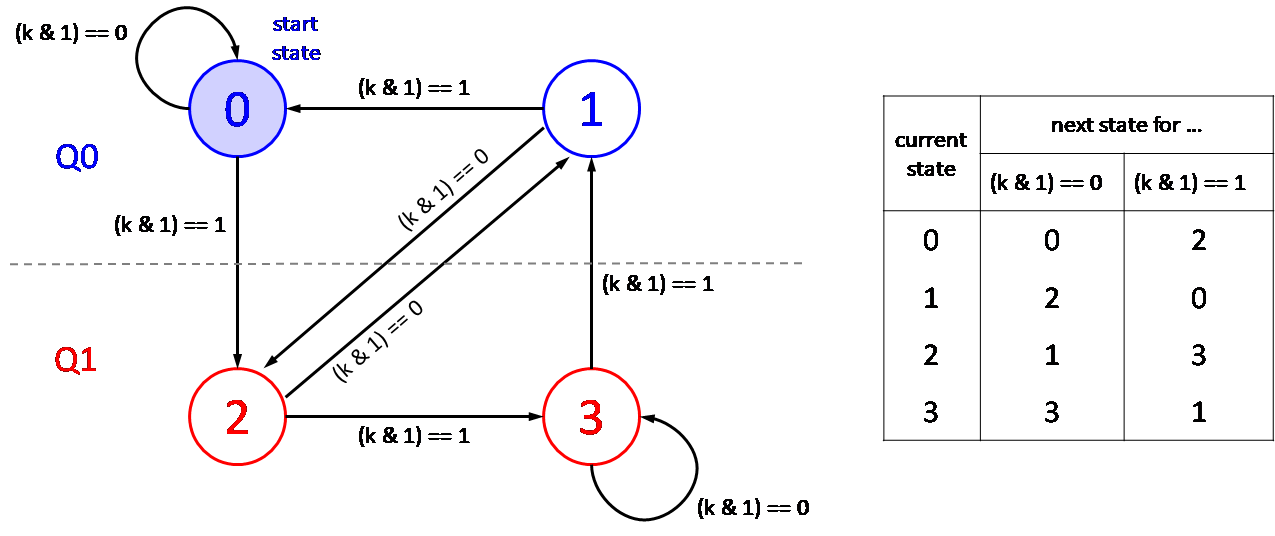
\includegraphics[width=.40\textwidth]{Quant_II/DepQuant.png}
\end{figure}
\item Encoder: \textit{Can} use trellis quantization, Viterbi algorithm. Not 
part of the standard:
\begin{figure}
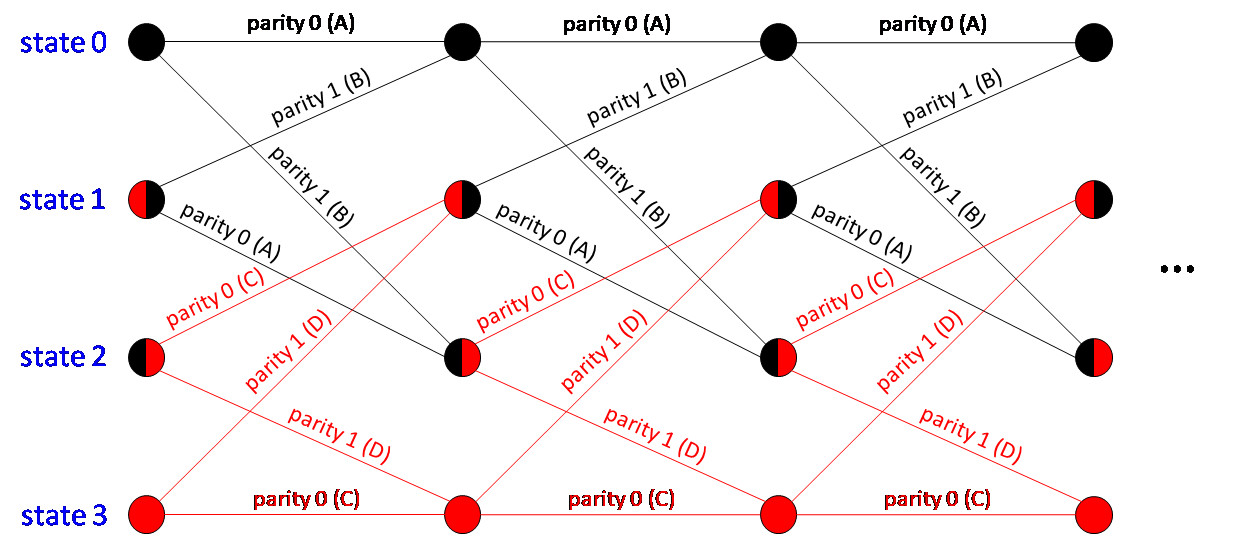
\includegraphics[width=.30\textwidth]{Quant_II/trellis.png}
\end{figure}
\eit
\end{frame}

\begin{frame}{Review of last lecture II}
\loud{Scalar quantization:}
\bit
\item  Treat one-dimensional sources. General case of vector quantization later.  
\item Model case: Sources $X$ with a probability density function $f_X=f$. 
\eit

\loud{Fixed rate quantization:}
\bit
\item Transmit all quantization indices with the same rate $R$.
\item [\iarrow] Fix number  $K=2^R$ of \loud{reconstruction points}. Then  determine optimal reconstruction points $s_k$ and optimal \loud{decision thresholds} 
$u_k$, $k=1,\dots,K$  by minimizing distortion.   
\item The $s_k$ need to satisfy the \loud{centroid condition}, if $u_k$ are given. 
\item The $u_k$ need to satisfy the \loud{nearest neighbor condition}, if $s_k$ are given 
\item \loud{Lloyd algorithm: } Iterative algorithm to approximately realize centroid and nearest neighbor condition.
\item Optimal quantizer often called \loud{Lloyd quantizer}.
\eit
\ALERT{Now: Allow entropy coding/lossless coding of quantization indices $\mathsf{i}$.} 
\end{frame}

\section{Entropy-Constrained Scalar Quantizer}
\begin{frame}
 \vspace{12.0ex}
\begin{center}
\begin{beamercolorbox}[sep=12pt,center]{part title}
\usebeamerfont{section title}\insertsection\par
\end{beamercolorbox}
\end{center}
\end{frame}

      

\begin{frame}{Rate-Distortion Efficiency of Scalar Quantizers}
  \vspace{-1.0ex}
  \STRUC{Distortion}
  \bit
\item Quantifies deviation between original and reconstructed samples
\item Typically: Additive distortion measures with $d(s,s')$ being the single-sample distortion
  \vspace{-1.0ex}$$
  D=\EV{d(S,S')}=\sum_{\forall k}\int_{u_k}^{u_{k+1}}d(s,s'_k)\,f(s)\;\d s
  $$
  \eit
  \vspace{-1.0ex}%
  \uncover<2->{\STRUC{Bit Rate}
  \bit
\item Average number of bits for coding quantization indexes $q$ (or reconstructed values $s'$)
  \vspace{-.5ex}$$
  R
  =\EV{\ell(S')}
  =\sum_{\forall k}p_k\cdot\ell_k
  =\sum_{\forall k}\ell_k\int_{u_k}^{u_{k+1}}f(s)\;\d s
  $$
  \eit}
  \vspace{-0.5ex}%
  \uncover<3->{\STRUC{Design of Scalar Quantizers}
  \bit
\item Lloyd quantizer minimizes distortion, but ignores impact on bit rate (assumes fixed-length coding)
  \item<4->[\iarrow] Improved performance: \loud{Consider bit rate in quantizer design}
  \eit}\vspace{1.0ex}
\end{frame}



  \subsection{Lagrangian Optimization}
      

\begin{frame}{Joint Minimization of Distortion and Bit Rate}
  \STRUC{Constrained Optimization Problem}
  \bit
\item Optimization problem can be formulated as 
  \vspace{-0.5ex}$$\min\;D\qquad\text{subject to}\qquad R\leq R_{\text{target}}$$
  \vspace{-2.75ex}or, equivalently,
  $$\min\;R\qquad\text{subject to}\qquad D\leq D_{\text{target}}$$
  \eit
  \bigskip
  \uncover<2->{%
    \STRUC{Reformulation as Unconstrained Problem}
    \bit
    \item Typically, constrained optimization problems cannot be solved directly
    \item Use technique of Lagrange multipliers for reformulation as unconstrained problem
      $$
      \min\;D+\lambda\cdot R
      $$
      \bit\relsize{1}\itemMode{arrow}
    \item<3->\vspace{-3ex} The parameter $\lambda>0$ is called \loud{Lagrange multiplier}
    \item<3-> Each value of $\lambda$ corresponds to a rate constraint $R_{\text{target}}$ (or distortion constraint $D_{\text{target}}$)
      \eit
    \eit
    }
\end{frame}



      

\begin{frame}{Convex Optimization: Illustration}
  \vspace{-2ex}
\begin{center}
\hfitbox{0.65\textwidth}{%
  \begin{tikzpicture}
     \begin{axis}[
        compat=newest,
        width=8cm,height=7cm,
        axis lines=none,
        xmin=-0.5,xmax=1.1,ymin=-0.3,ymax=1.1,
        clip mode=individual, % ensures curves are plot one after another
        after end axis/.code={
          \draw[->,style={-{Latex[length=2.5mm,width=1.5mm]},line width=0.75pt}] 
               (axis cs: -0.5,0) -- (axis cs: 1.2,0);
          \draw[->,style={-{Latex[length=2.5mm,width=1.5mm]},line width=0.75pt}] 
               (axis cs: 0,-0.1) -- (axis cs: 0,1.1);
          \node[black, anchor=north east] at (axis cs: 0,1.1) {$D$};
          \node[black, anchor=north east] at (axis cs: 1.3,0) {$R$};
        }
     ]
     \pgfmathsetmacro{\a}{30}
     \pgfmathsetmacro{\ex}{-2.5}
     \pgfmathsetmacro{\rt}{ln(-tan(\a)/\ex)/\ex}
     \pgfmathsetmacro{\la}{tan(\a)}
     \pgfmathsetmacro{\xx}{(\rt-\la*exp(\ex*\rt))/(1+\la*\la)}
     \addplot[name path=func,myblue!20,samples=101,domain=0.0:1.1,line width=1.0pt,mark=none] 
              {exp(\ex*x)};
     \path[name path=axis] (axis cs: 0,1) -- (axis cs: 1.1,1);
     \addplot[myblue!20] fill between[of=func and axis,soft clip={domain=0:1.1}];
     \begin{scope}[visible on=<4->]
        \addplot[mygreen,samples=101,domain=-0.5:1.0,line width=1.0pt,mark=none]
           {\ex*exp(\ex*\rt)*x}; 
        \draw[mygreen,domain={180-\a}:180] plot (axis cs: {0.4*cos(\x)},{0.4*sin(\x)});
        \node[mygreen] at (axis cs: {0.25*cos(180-0.5*\a)},{0.25*sin(180-0.5*\a)}) 
             {$\alpha$};
        \node[mygreen,anchor=south west] at (axis cs: -0.5,{-0.5*\ex*exp(\ex*\rt)}) 
             {$-\lambda\cdot R$};
        \node[mygreen,anchor=north west] at (axis cs: -0.5,-0.1)
             {$\lambda=\tan\alpha$};
        \draw[vividviolet,line width=1.0pt] 
             (axis cs: {\xx},{\ex*exp(\ex*\rt)*\xx}) -- (axis cs: {\rt},{exp(\ex*\rt)});
        \node[myviolet,anchor=south east] 
             at (axis cs: {0.5*\rt+0.5*\xx},{(0.5*\rt+0.5*\xx)/\la+exp(\ex*\rt)-\rt/\la})
             {$C$};
     \end{scope}
     \begin{scope}[visible on=<5->]
        \addplot[myblue,samples=101,domain=0.0:1.1,line width=1.0pt,mark=none] 
                {exp(\ex*x)};
        \node[anchor=east] at (axis cs:-0.1, 0.7) {%
          \color{myblue}\small convex hull};
        \draw[myblue,-{Latex[length=2.5mm,width=1.2mm]},line width=0.5pt]
        (-0.1,0.7) -- ({ln(0.7)/\ex},{0.7});
     \end{scope}
     \begin{scope}[visible on=<2->]
        \draw[myred,line width=1.0pt] 
             (axis cs: {\rt},-0.05) -- (axis cs: {\rt},1.1);
        \node[myred,anchor=north west] at (axis cs: {\rt-0.02},-0.03) {$R_{\text{target}}$};
     \end{scope}
     \begin{scope}[visible on=<3->]
       \draw[myred,fill] (axis cs:  {\rt},{exp(\ex*\rt)}) circle [radius=2.5pt];
       \node[myred,anchor=south west,yshift=-.5ex] at (axis cs: 0.8,0.45) {%
         \color{myred}\small solution of constrained problem
       };
       \draw[myred,-{Latex[length=2.5mm,width=1.2mm]},line width=0.5pt]
       (0.8,0.45) -- ({\rt+0.02},{exp(\ex*\rt)+0.02});
     \end{scope}
     \node[anchor=north west,align=left] at (axis cs: 1.12,1.1) {%
       \color{myblue}\small region of achievable\\
       \color{myblue}\small rate-distortion points\\
       \color{myblue}\small for scalar quantizer\\
       };
     \end{axis}
  \end{tikzpicture}
}
\end{center}
\vspace{-1ex}
\bit\TabPositions{12em}
  \item<6->[\iarrow] Points on \textcolor{myblue}{convex hull}:\tab Minimize \textcolor{myviolet}{distance $C$} to line \textcolor{mygreen}{$D=-\lambda\cdot R$}
  \item<7->[\iarrow] Geometrical interpretation:\tab Rotate coordinate system by \textcolor{mygreen}{angle $\alpha$}
\eit\vspace{-5ex}
\end{frame}



      

\begin{frame}{Convex Optimization: Lagrangian Formulation}
\vspace{-2.5ex}
\begin{center}
\hfitbox{0.62\textwidth}{%
  \relsize{-1}%
  \begin{tikzpicture}
     \pgfmathsetmacro{\r}{0.5}
     \pgfmathsetmacro{\d}{0.7}
     \pgfmathsetmacro{\a}{30}
     \pgfmathsetmacro{\ex}{-2.5}
     \pgfmathsetmacro{\rt}{ln(-tan(\a)/\ex)/\ex}
     \pgfmathsetmacro{\la}{tan(\a)}
     \pgfmathsetmacro{\ca}{cos(\a)}
     \pgfmathsetmacro{\sa}{sin(\a)}
     \pgfmathsetmacro{\xx}{(\rt-\la*exp(\ex*\rt))/(1+\la*\la)}
     \begin{axis}[
        compat=newest,
        width=8cm,height=6cm,
        axis lines=none,
        xmin=-0.5,xmax=1.1,ymin=-0.1,ymax=1.1,
        clip mode=individual, % ensures curves are plot one after another
        after end axis/.code={
          \draw[->,style={-{Latex[length=2.5mm,width=1.5mm]},line width=0.5pt}] 
               (axis cs: {-0.1*\ca},{-0.1*\sa}) -- (axis cs: {1.2*\ca},{1.2*\sa});
          \draw[->,style={-{Latex[length=2.5mm,width=1.5mm]},line width=0.5pt}] 
               (axis cs: {0.1*\sa},{-0.1*\ca}) -- (axis cs: {-1.2*\sa},{1.2*\ca});
          \node[black, anchor=north west] at (axis cs: {1.2*\ca},{1.2*\sa}) {$R$};
          \node[black, anchor=north east] at (axis cs: {-1.2*\sa},{1.2*\ca}) {$D$};
          \draw[mygreen,line width=1.0pt] 
               (axis cs: -0.7,0) -- (axis cs: 1.1,0);
          \node[mygreen, anchor=south west] at (axis cs: -0.7,0) {$-\lambda\cdot R$};
        }
     ]
       \draw[mygreen,domain=0:{0+\a}] plot (axis cs: {0.3*cos(\x)},{0.3*sin(\x)});
       \node[mygreen] at (axis cs: {0.2*cos(0+0.5*\a)},{0.2*sin(0+0.5*\a)}) 
            {$\alpha$};
     \addplot[name path=func,myblue,samples=101,domain=0.0:1.2,line width=1.0pt,mark=none] 
              ( {\ca*x-\sa*exp(\ex*x)}, {\ca*exp(\ex*x)+\sa*x} );
     \path[name path=axis] (axis cs: -0.5,0.95) -- (axis cs: 1,0.95);
     \addplot[myblue!20] fill between[of=func and axis,
       soft clip={domain=-1:1}];
     \draw[myred,fill] (axis cs:  {\ca*\rt-\sa*exp(\ex*\rt)}, {\ca*exp(\ex*\rt)+\sa*\rt}) circle [radius=2pt];
     \begin{scope}[visible on=<2->]
       \draw[myviolet,->,style={-{Latex[length=2.5mm,width=1.5mm]},line width=0.75pt}] 
       (axis cs: 0.0,-0.1) -- (axis cs: 0.0,1.1);
       \node[myviolet, anchor=north east] at (axis cs: 0,1.1) {$C$};
     \end{scope}
     \begin{scope}[visible on=<4->]
        \draw[gray,line width=0.5pt] 
             (axis cs: {\ca*\r-\sa*\d},{\ca*\d+\sa*\r}) -- (axis cs: {-\sa*\d},{\ca*\d});
        \draw[gray,line width=0.5pt] 
             (axis cs: {\ca*\r-\sa*\d},{\ca*\d+\sa*\r}) -- (axis cs: {\ca*\r},{\sa*\r});
     \end{scope}
     \begin{scope}[visible on=<5->]
        \draw[gray,line width=0.5pt] 
             (axis cs: {\ca*\r-\sa*\d},{\ca*\d}) -- (axis cs: {-\sa*\d},{\ca*\d});
        \draw[gray,line width=0.5pt] 
             (axis cs: {\ca*\r-\sa*\d},{\ca*\d}) -- (axis cs: {\ca*\r-\sa*\d},{\ca*\d+\sa*\r});
        \draw[mygreen,domain=90:{90+\a}] plot (axis cs: {0.3*cos(\x)},{0.3*sin(\x)});
        \node[mygreen] at (axis cs: {0.2*cos(90+0.5*\a)},{0.2*sin(90+0.5*\a)}) 
              {$\alpha$};
        \draw[mygreen,domain=0:{\a}] plot 
             (axis cs: {-\sa*\d+0.2*cos(\x)},{\ca*\d+0.2*sin(\x)});
        \node[mygreen] at 
             (axis cs: {-\sa*\d+0.13*cos(0.5*\a)},{\ca*\d+0.13*sin(0.5*\a)})
              {$\alpha$};
     \end{scope}
     \begin{scope}[visible on=<6->]
        \draw[gray,dashed,line width=0.5pt] 
           (axis cs: {\ca*\r-\sa*\d},{\ca*\d}) -- (axis cs: 0.65,{\ca*\d});
        \draw[myred,<->,style={{Latex[length=2.5mm,width=1.2mm]}-{Latex[length=2.5mm,width=1.2mm]},line width=0.5pt}] 
               (axis cs: 0.5,{\ca*\d}) -- (axis cs: 0.5,0);
        \node[myred,anchor=west] at (axis cs: 0.5,{0.35*\ca*\d}) {$D\cdot\cos\alpha$};
     \end{scope}
     \begin{scope}[visible on=<7->]
        \draw[gray,dashed,line width=0.5pt] 
           (axis cs: 0,{\ca*\d+\sa*\r}) -- (axis cs: 0.65,{\ca*\d+\sa*\r});
        \draw[myred,<->,style={{Latex[length=2.5mm,width=1.2mm]}-{Latex[length=2.5mm,width=1.2mm]},line width=0.5pt}] 
               (axis cs: 0.5,{\ca*\d}) -- (axis cs: 0.5,{\ca*\d+\sa*\r});
        \node[myred,anchor=west] at (axis cs: 0.5,{\ca*\d+0.5*\sa*\r}) {$R\cdot\sin\alpha$};
     \end{scope}
     \begin{scope}[visible on=<3->]
        \draw[black,fill] 
             (axis cs: {\ca*\r-\sa*\d},{\ca*\d+\sa*\r}) circle [radius=2pt];
     \end{scope}
  \end{axis}
  \end{tikzpicture}
}
\end{center}
\vspace{-1.5ex}
\bit\TabPositions{11em}
  \item<8->[\iarrow] Minimize distance: \tab$C=D\cdot\cos\alpha+R\cdot\sin\alpha$
  \item<9->[\iarrow] Equivalent minimization: \tab\textcolor{myred}{$J=D+\lambda\cdot R$}\qquad(note: Lagrange multiplier is given by $\lambda=\tan\alpha$)
\eit\vspace{-5ex}
\end{frame}


  \subsection{Optimization Criterions}
      

\begin{frame}{Optimal Scalar Quantizer}
  \STRUC{Optimization Criterion}
  \bit
\item Minimization of Lagrangian cost for some given Lagrange multiplier $\lambda$
  \vspace{-1ex}\begin{align*}
    J
    &\;=\;D+\lambda\cdot R\\[.5ex]
    \onslide<2->
    &\;=\;
    \sum_{\forall k}\int_{u_k}^{u_{k+1}}d(s,s'_k)\,f(s)\;\d s
    +
    \lambda
    \sum_{\forall k}\ell_k\int_{u_k}^{u_{k+1}}f(s)\;\d s
    &&\quad\text{\small(any additive distortion measure)}
    \onslide
  \end{align*}
  \item<3->[\iarrow] Each Lagrange multiplier $\lambda>0$ yields solution of original constrained problem for one $R_{\text{target}}$
  \eit

  \medskip
  \uncover<4->{\STRUC{Optimization Criterion for MSE Distortion}
  \bit
\item Determine quantizer parameters ($s'_k$ and $u_k$) and codeword lengths $\ell_k$ such that\\[.25ex]
  the Lagrangian cost $J=D+\lambda R$ for MSE distortion is minimized
  \begin{align*}
    J
    &\;=\;
    \sum_{\forall k}\int_{u_k}^{u_{k+1}}(s-s'_k)^2\,f(s)\;\d s
    +
    \lambda
    \sum_{\forall k}\ell_k\int_{u_k}^{u_{k+1}}f(s)\;\d s
  \end{align*}
  \eit}\vspace {-5ex}
\end{frame}



      

\begin{frame}{Optimal Decoder Mapping:~ Centroid Condition}
  \vspace{-1.0ex}
  $$
  J\,=\,\sum_{\forall k}\int_{u_k}^{u_{k+1}}(s-s'_k)^2\,f(s)\;\d s
  \;+\;\lambda\cdot\sum_{\forall k}\ell_k\int_{u_k}^{u_{k+1}}f(s)\;\d s
  $$
  \medskip
  \ben
\item<+-> \STRUC{Optimize reconstruction levels $s'_k$} for given decision thresholds $u_k$
  \bit\relsize{1}
\item<+->Note: Rate term does not depend on reconstruction levels $s'_k$
\item<+->[\iarrow] Same condition as for Lloyd quantizer
  \eit
  \een
  \vspace{-1ex}
  \bit
\item<+->[\iarrow]\smallskip \STRUC{Centroid condition for MSE distortion}
  \bit\relsize{1}
\item<.-> Optimal reconstruction level $s'_k$ is given by conditional mean
  \eit
  \vspace{.5ex}$$
  \boxed{\;s'_k
    = \EV{S\,\cond\,S\in\set{I}_k} 
    =  \int\limits_{u_k}^{u_{k+1}}s\, f(s\cond s\in\set{I}_k)\;\d s
    =  \frac{1}{p_k}\int\limits_{u_k}^{u_{k+1}}s\, f(s)\;\d s
    =
    \frac{\displaystyle\int_{u_k}^{u_{k+1}}s\, f(s)\;\d s}
 	 {\displaystyle\int_{u_k}^{u_{k+1}}f(s)\;\d s}\;}
  $$
  \eit\vspace{-10ex}
\end{frame}

      

\begin{frame}{Optimal Lossless Mapping: ~Entropy Condition}
  \vspace{-1.0ex}
  $$
  J\,=\,\sum_{\forall k}\int_{u_k}^{u_{k+1}}(s-s'_k)^2\,f(s)\;\d s
  \;+\;\lambda\cdot\sum_{\forall k}\ell_k\int_{u_k}^{u_{k+1}}f(s)\;\d s
  $$
  \medskip
  \ben\setcounter{enumi}{1}
\item<+-> \STRUC{Optimize codeword lengths $\ell_k$} for given decision thresholds $u_k$
  \bit\relsize{1}
\item<+->Note: Distortion term does not depend on codeword lengths $\ell_k$
\item<+->[\iarrow] Remember: Lossless coding theorem: $R\geq H(S')$
  \vspace{-.0ex}$$
  \sum_{\forall k}p_k\cdot\ell_k \geq -\sum_{\forall k}p_k\cdot\log_2p_k
  \quad\qquad(\text{equality if and only if $\ell_k=-\log_2p_k$})
  $$
  \eit
  \een
  \vspace{-3ex}
  \bit
\item<+->[\iarrow] \STRUC{Entropy condition} (neglecting inefficiency of actual entropy coding)
 \vspace{-0.5ex}$$
    \boxed{\;\ell_k=-\log_2p_k
    =-\log_2\!\left(\int_{u_k}^{u_{k+1}}f(s)\;\d s\right)\;}
  $$
\eit\vspace{-10ex}
\end{frame}

      

\begin{frame}{Optimal Encoder Mapping:~ Condition for Decision Thresholds}


  \vspace{-1.0ex}
  $$
  J\,=\,\sum_{\forall k}\int_{u_k}^{u_{k+1}}(s-s'_k)^2\,f(s)\;\d s
  \;+\;\lambda\cdot\sum_{\forall k}\ell_k\int_{u_k}^{u_{k+1}}f(s)\;\d s
  $$
  \medskip

\bit
\item
Taking derivative with respect to $u_k$: 
\begin{align*}
0\stackrel{!}{=}&\frac{\partial}{\partial u_k}J\\
=&(u_k-s'_{k-1})^2f(u_k)+\lambda\ell_{k-1}f(u_k)-(u_k-s'_k)^2f(u_k)-\lambda\ell_{k}f(u_k).
\end{align*}
\item[\iarrow]Thus, necessary condition for optimal decistion thresholds is: 
\begin{align*}
(u_k-s'_{k-1})^2+\lambda\ell_{k-1}=(u_k-s'_k)^2+\lambda\ell_{k}.
\end{align*}

\eit

%  \vspace{-1.0ex}
%  $$
%  J\,=\,\sum_{\forall k}\int_{u_k}^{u_{k+1}}(s-s'_k)^2\,f(s)\;\d s
%  \;+\;\lambda\cdot\sum_{\forall k}\ell_k\int_{u_k}^{u_{k+1}}f(s)\;\d s
%  $$
%  \medskip
%  \ben\setcounter{enumi}{2}
%\item<+-> \STRUC{Optimize decision thresholds $u_k$} for given reconstruction levels $s'_k$ and codeword lengths $\ell_k$
%  \begin{minipage}[t]{0.5\linewidth}
%    \vspace{-1.0ex}
%    \bit\relsize{1}
%    \item<+-> Note: Each threshold $u_k$ impacts only neighbouring intervals $\set{I}_{k-1}$ and $\set{I}_k$
%    \item[\iarrow]<+-> Map each input value $s$ to interval $\set{I}_k$ that minimizes
%      contribution to Lagrangian cost
%      \vspace{-.5ex}$$J(s\cond\set{I}_k)=(s-s'_k)^2+\lambda\cdot\ell_k$$
%    \item[\iarrow]<+->\vspace{-.5ex} At decision threshold $u_k$, we require
%      \vspace{-.5ex}$$J(u_k\cond\set{I}_{k-1})=J(u_k\cond\set{I}_k)$$
%  \eit
%  \end{minipage}%
%  \begin{minipage}[t]{0.5\linewidth}
%    \vskip0pt%
%    \begin{flushright}
%      \uncover<3->{\hfitbox{0.88\textwidth}{%
%        \begin{tikzpicture}
%          \begin{axis}[
%              compat=newest,
%              width=8cm,height=7cm,
%              axis lines=none,
%              xmin=-0.5,xmax=1.1,ymin=-0.3,ymax=1.0,
%              clip mode=individual, % ensures curves are plot one after another
%              after end axis/.code={
%                \draw[->,style={-{Latex[length=2.5mm,width=1.5mm]},line width=0.75pt}] 
%                (axis cs: -0.5,0) -- (axis cs: 1.2,0);
%                \draw[->,style={-{Latex[length=2.5mm,width=1.5mm]},line width=0.75pt}] 
%                (axis cs: -0.45,-0.05) -- (axis cs: -0.45,1.1);
%                \node[black, anchor=north east] at (axis cs: -0.45,1.1) {$J\,$};
%                \node[black, anchor=north west] at (axis cs: 1.2,0) {$\!\!s$};
%              }
%            ]
%            \pgfmathsetmacro{\uk}{0.298}
%            \addplot[myblue,samples=101,domain=-0.5:1.1,line width=1.0pt,mark=none] 
%                    {3*(x+0.1)^2+0.2};
%            \draw[myblue,line width=1.0pt] (-0.1,0) -- (-0.1,0.2);
%            \node[myblue,anchor=north] at (-0.1,0) {$s'_{k-1}$};
%            \node[myblue,anchor=east] at (-0.1,0.1) {$\lambda\cdot\ell_{k-1}$};
%            \node[myblue,anchor=west] at (-0.4,0.5) {$J(s\cond\set{I}_{k-1})$};
%            \addplot[mygreen,samples=101,domain=-0.5:1.1,line width=1.0pt,mark=none] 
%                    {3*(x-0.6)^2+0.4};
%            \draw[mygreen,line width=1.0pt] (0.6,0) -- (0.6,0.4);
%            \node[mygreen,anchor=north] at (0.6,0) {$s'_{k}$};
%            \node[mygreen,anchor=west] at (0.6,0.175) {$\lambda\cdot\ell_{k}$};
%            \node[mygreen,anchor=east] at (1.0,0.93) {$J(s\cond\set{I}_k)$};
%            \begin{scope}[visible on=<4->]
%            \draw[myred,line width=1.0pt] 
%                    (axis cs: {\uk},-0.025) -- (axis cs: {\uk},1.0);
%            \node[myred,anchor=north] at (axis cs: {\uk},-0.025) {$u_k$};
%            \end{scope}
%          \end{axis}
%        \end{tikzpicture}%
%      }}
%    \end{flushright}
%  \end{minipage}
%  \een\vspace{-3ex}
\end{frame}



      


\begin{frame}{Optimal Encoder Mapping:~ Modified Nearest Neighbour Condition}
\vspace{-1ex}\bit
\item<+-> Optimal encoding mapping for MSE distortion
\begin{align*}
(u_k-s'_{k-1})^2+\lambda\cdot\ell_{k-1} =&(u_k-s'_k)^2+\lambda\cdot\ell_k
\\ 
\iff u_k^2-2u_ks'_{k-1}+(s'_{k-1})^2+\lambda\cdot\ell_{k-1} = &u_k^2-2u_ks'_k+(s'_{k})^2+\lambda\cdot\ell_{k}
\\
\iff 2u_k(s'_k-s'_{k-1})=&(s'_k)^2-(s'_{k-1})^2+\lambda\,(\ell_k-\ell_{k-1})
\\
\iff 2u_k(s'_k-s'_{k-1}) = &(s'_k-s'_{k-1})(s'_k+s'_{k-1})+\lambda\,(\ell_k-\ell_{k-1})
\end{align*}

%
%  \vspace{-1ex}\beqan
%    J(u_k\cond\set{I}_{k-1})
%    &\!\!\!=\!\!\!&
%        J(u_k\cond\set{I}_k)\\[.5ex]
%  \uncover<+->{
%    (u_k-s'_{k-1})^2+\lambda\cdot\ell_{k-1}
%    &\!\!\!=\!\!\!&
%        (u_k-s'_k)^2+\lambda\cdot\ell_k\\[.5ex]}
%  \uncover<+->{
%    u_k^2-2u_ks'_{k-1}+(s'_{k-1})^2+\lambda\cdot\ell_{k-1}
%    &\!\!\!=\!\!\!&
%        u_k^2-2u_ks'_k+(s'_{k})^2+\lambda\cdot\ell_{k}\\[.5ex]}
%  \uncover<+->{
%    2u_k(s'_k-s'_{k-1})
%    &\!\!\!=\!\!\!&
%       (s'_k)^2-(s'_{k-1})^2+\lambda\,(\ell_k-\ell_{k-1})\\[.5ex]}
%  \uncover<+->{
%    2u_k(s'_k-s'_{k-1})
%    &\!\!\!=\!\!\!&
%       (s'_k-s'_{k-1})(s'_k+s'_{k-1})+\lambda\,(\ell_k-\ell_{k-1})}
%  \eeqan
\item[\iarrow]<+->\bigskip \loud{Modified nearest neighbour condition for MSE distortion}
  $$
  \boxed{\;u_k = \frac{1}{2}\,\big(s'_{k-1}+s'_k)+
        \frac{\lambda}{2}\,\left(\frac{\ell_k-\ell_{k-1}}{s'_k-s'_{k-1}}\right)\;}
  $$
\item[\ALERT{\iarrow}]<+->\smallskip \ALERT{Threshold is shifted towards the reconstruction level with the longer codeword}
\eit\vspace{-5ex}
\end{frame}

      
  \subsection{Entropy-Constrained Lloyd Algorithm}
  

\begin{frame}{Entropy-Constrained Lloyd Quantizer: Minimization of Lagrangian Cost}
\STRUC{Necessary Conditions for Optimality (MSE distortion)}
\ben
\item Centroid condition
  $$
s'_k
     =
     \frac{\int_{u_k}^{u_{k+1}}s\, f(s)\;\d s}
 	     {\int_{u_k}^{u_{k+1}}f(s)\;\d s}
  $$
\item Entropy condition
  $$
    \ell_k=-\log_2p_k
  $$
\item Modified nearest neighbor condition
  $$
u_k = \frac{1}{2}\,\big(s'_{k-1}+s'_k)+
        \frac{\lambda}{2}\,\left(\frac{\ell_k-\ell_{k-1}}{s'_k-s'_{k-1}}\right)
  $$
\een
\uncover<2->{
\STRUC{Design of optimal entropy-constrained scalar quantizers}
\bit
  \item In general: Cannot be derived in closed form 
  \item[\iarrow] Iterative algorithm similar to Lloyd algorithm
\eit}\vspace{-5ex}
\end{frame}

  

\begin{frame}{Entropy-Constrained Lloyd Algorithm for Given Pdf~ (MSE Distortion)}
  \vspace{-1ex}Given is:
  \begin{minipage}[t]{0.8\linewidth}
    \vskip-1.5ex%
\bit\itemMode{circle}
\item<+-> the marginal probability density function $f(s)$ of the source
\item<.-> a Lagrange multiplier $\lambda>0$
  \eit
  \end{minipage}
  
\medskip
\uncover<+->{\STRUC{Iterative quantizer design}}
\ben
\item<.-> Choose an initial set of reconstruction levels~$\{s'_k\}$ and codeword lengths $\{\ell_k\}$
\item<+->\smallskip Update the decision thresholds $\{u_k\}$ according to
	{\vspace{-.5ex}\[
          u_k = \frac{1}{2}\,\big(s'_{k-1}+s'_k)+
          \frac{\lambda}{2}\,\left(\frac{\ell_k-\ell_{k-1}}{s'_k-s'_{k-1}}\right)
	\]}
\item<+-> Update the reconstruction levels~$\{s'_k\}$ and codeword lengths $\{\ell_k\}$ according to
	{\vspace{-.5ex}\[
	s'_k=\frac{\int_{u_k}^{u_{k+1}}s\,f(s)\;\d s}
              {\int_{u_k}^{u_{k+1}}f(s)\;\d s}
	      \quad\qquad\text{and}\qquad\quad
              \ell_k=-\log_2\!\left(\int_{u_k}^{u_{k+1}}f(s)\;\d s\right)
	\]}
\item<+-> Repeat the previous two steps until convergence
\een
\end{frame}

  

\begin{frame}{Entropy-Constrained Lloyd Algorithm for a Training Set~ (MSE Distortion)}
  \vspace{-1ex}Given is:
  \begin{minipage}[t]{0.8\linewidth}
    \vskip-1.5ex%
\bit\itemMode{circle}
\item<+-> a sufficiently large realization $\{s_n\}$ of the considered source
\item<.-> a Lagrange multiplier $\lambda>0$
  \eit
  \end{minipage}
  
\medskip
\uncover<.->{\STRUC{Iterative quantizer design}}
\ben
\item<.-> Choose an initial set of reconstruction levels~$\{s'_k\}$ and codeword lengths $\{\ell_k\}$
\item<+->\smallskip Associate all samples of the training set $\{s_n\}$ with one of quantization intervals $\set{I}_k$
  {\[
    q(s_n)=\arg\,\min_{\forall k}\;\;(s_n-s'_k)^2+\lambda\cdot\ell_k
	\]}
\item<+-> Update the reconstruction levels~$\{s'_k\}$ and codeword lengths $\{\ell_k\}$ according to
	{\vspace{-.5ex}\[
	s'_k=\frac{1}{N_k}\sum_{n:\;q(s_n)=k}s_n
	\quad\qquad\text{and}\qquad\quad
        \ell_k=-\log_2\!\left(\frac{N_k}{N}\right)
	      \]}
        where $N_k$ is the number of samples associated with $\set{I}_k$
        and $N$ is the total number of samples
\item<+->\smallskip Repeat the previous two steps until convergence
\een
\end{frame}




\begin{frame}{Example: EC Lloyd Algorithm for Gaussian Source}
  \begin{minipage}{0.5\linewidth}
    Gaussian Source
    \bit
  \item Zero mean $\mu=0$
    \item Unit variance $\sigma^2=1$
      \eit

      \bigskip\bigskip
\STRUC{EC Lloyd Quantizer for 2 bits per sample}
\bit\TabPositions{10em}
\item Decision thresholds:\tab\hspace{-2.0ex}%
  {\begin{tabular}[t]{r@{\;\;}c@{\;\;}l}
  $u_{0/1}$  &$=$& $\pm0.538$\\
  $u_{-1/2}$ &$=$& $\pm1.623$\\
  $u_{-2/3}$ &$=$& $\pm2.743$\\
  $u_{-3/4}$ &$=$& $\pm3.926$
  \end{tabular}}
\item\smallskip Reconstruction levels:\tab
  {\begin{tabular}[t]{r@{\;\;}c@{\;\;}l}
  $s'_0$     &$=$& $\phantom{\pm}0.000$\\[.2ex]
  $s'_{\pm1}$ &$=$& $\pm0.980$\\
  $s'_{\pm2}$ &$=$& $\pm1.981$\\
  $s'_{\pm3}$ &$=$& $\pm3.029$\\
  $s'_{\pm4}$ &$=$& $\pm4.148$\\
  \end{tabular}}
  \eit
  \end{minipage}%
  \begin{minipage}{0.5\linewidth}
    \begin{center}
    \hfitbox{\linewidth}{%
  \begin{tikzpicture}
     \begin{axis}[
        compat=newest,
        width=9cm,height=7cm,
        axis lines=none,
        xmin=-5,xmax=5,ymin=-0.15,ymax=0.45,
        clip mode=individual, % ensures curves are plot one after another
        after end axis/.code={
          \draw[->,style={-{Latex[length=2.5mm,width=1.2mm]},line width=0.5pt}] 
               (axis cs: -5,0) -- (axis cs: 5,0);
          %\node[black, anchor=north east] at (axis cs: 5,-0.01) {$s$};
        }
     ]
       \addplot[name path=func,black,samples=101,domain=-5:5,line width=0.5pt,mark=none]
               {0.39894228040143267793994605993438*exp(-0.5*x*x)};
       \path[name path=axis] (axis cs: -5,0) -- (axis cs: 5,0);
       \node[anchor=north west,yshift=-.5ex,xshift=-1.0ex] at (axis cs: 5,0) {$s$};
       \addplot[green!20]       fill between[of=func and axis,soft clip={domain=-5.000:-3.926}];
       \addplot[myviolet!20]    fill between[of=func and axis,soft clip={domain=-3.926:-2.743}];
       \addplot[blue!20]        fill between[of=func and axis,soft clip={domain=-2.743:-1.623}];
       \addplot[red!20]         fill between[of=func and axis,soft clip={domain=-1.623:-0.538}];
       \addplot[green!20]       fill between[of=func and axis,soft clip={domain=-0.538: 0.538}];
       \addplot[red!20]         fill between[of=func and axis,soft clip={domain= 0.538: 1.623}];
       \addplot[blue!20]        fill between[of=func and axis,soft clip={domain= 1.623: 2.743}];
       \addplot[myviolet!20]    fill between[of=func and axis,soft clip={domain= 2.743: 3.926}];
       \addplot[green!20]       fill between[of=func and axis,soft clip={domain= 3.926: 5.000}];

       \pgfmathsetmacro{\su}{0.52}
       \pgfmathsetmacro{\ou}{-0.05}
       \begin{scope}
         \addplot[line width=0.5pt,dashed] coordinates { (-3.926,{\ou}) (-3.926,{\su}) };
         \addplot[line width=0.5pt,dashed] coordinates { (-2.743,{\ou}) (-2.743,{\su}) };
         \addplot[line width=0.5pt,dashed] coordinates { (-1.623,{\ou}) (-1.623,{\su}) };
         \addplot[line width=0.5pt,dashed] coordinates { (-0.538,{\ou}) (-0.538,{\su}) };
         \addplot[line width=0.5pt,dashed] coordinates { ( 0.538,{\ou}) ( 0.538,{\su}) };
         \addplot[line width=0.5pt,dashed] coordinates { ( 1.623,{\ou}) ( 1.623,{\su}) };
         \addplot[line width=0.5pt,dashed] coordinates { ( 2.743,{\ou}) ( 2.743,{\su}) };
         \addplot[line width=0.5pt,dashed] coordinates { ( 3.926,{\ou}) ( 3.926,{\su}) };
       \end{scope}
     
       \begin{scope}
         \node[anchor=north,yshift=-.3ex] at (axis cs: -3.926,{\ou}) {\small$u_{-3}$};
         \node[anchor=north,yshift=-.3ex] at (axis cs: -2.743,{\ou}) {\small$u_{-2}$};
         \node[anchor=north,yshift=-.3ex] at (axis cs: -1.623,{\ou}) {\small$u_{-1}$};
         \node[anchor=north,yshift=-.3ex] at (axis cs: -0.538,{\ou}) {\small$u_{0}$};
         \node[anchor=north,yshift=-.3ex] at (axis cs:  0.538,{\ou}) {\small$u_{1}$};
         \node[anchor=north,yshift=-.3ex] at (axis cs:  1.623,{\ou}) {\small$u_{2}$};
         \node[anchor=north,yshift=-.3ex] at (axis cs:  2.743,{\ou}) {\small$u_{3}$};
         \node[anchor=north,yshift=-.3ex] at (axis cs:  3.926,{\ou}) {\small$u_{4}$};
       \end{scope}

       \pgfmathsetmacro{\ss}{0.25}
       \pgfmathsetmacro{\os}{0.00}
       \begin{scope}
         \addplot[line width=1.0pt,mygreen]  coordinates { ( -4.148,{\os}) (-4.148,{\ss}) };
         \addplot[line width=1.0pt,myviolet] coordinates { ( -3.029,{\os}) (-3.029,{\ss}) };
         \addplot[line width=1.0pt,myblue]   coordinates { ( -1.981,{\os}) (-1.981,{\ss}) };
         \addplot[line width=1.0pt,myred]    coordinates { ( -0.980,{\os}) (-0.980,{\ss}) };
         \addplot[line width=1.0pt,mygreen]  coordinates { (  0.000,{\os}) ( 0.000,{\ss}) };
         \addplot[line width=1.0pt,myred]    coordinates { (  0.980,{\os}) ( 0.980,{\ss}) };
         \addplot[line width=1.0pt,myblue]   coordinates { (  1.981,{\os}) ( 1.981,{\ss}) };
         \addplot[line width=1.0pt,myviolet] coordinates { (  3.029,{\os}) ( 3.029,{\ss}) };
         \addplot[line width=1.0pt,mygreen]  coordinates { (  4.148,{\os}) ( 4.148,{\ss}) };

         \draw[fill,mygreen]  (axis cs: -4.148,{\ss}) circle [radius=2.5pt];
         \draw[fill,myviolet] (axis cs: -3.029,{\ss}) circle [radius=2.5pt];
         \draw[fill,myblue]   (axis cs: -1.981,{\ss}) circle [radius=2.5pt];
         \draw[fill,myred]    (axis cs: -0.980,{\ss}) circle [radius=2.5pt];
         \draw[fill,mygreen]  (axis cs:  0.000,{\ss}) circle [radius=2.5pt];
         \draw[fill,myred]    (axis cs:  0.980,{\ss}) circle [radius=2.5pt];
         \draw[fill,myblue]   (axis cs:  1.981,{\ss}) circle [radius=2.5pt];
         \draw[fill,myviolet] (axis cs:  3.029,{\ss}) circle [radius=2.5pt];
         \draw[fill,mygreen]  (axis cs:  4.148,{\ss}) circle [radius=2.5pt];
         
         \node[blue,anchor=north,yshift=-.0ex,xshift=-1.ex] at (axis cs: -4.148,{\os}) {\small$s'_{-4}$};
         \node[blue,anchor=north,yshift=-.0ex,xshift=-.5ex] at (axis cs: -3.029,{\os}) {\small$s'_{-3}$};
         \node[blue,anchor=north,yshift=-.0ex,xshift=-.5ex] at (axis cs: -1.981,{\os}) {\small$s'_{-2}$};
         \node[blue,anchor=north,yshift=-.0ex,xshift=-.5ex] at (axis cs: -0.980,{\os}) {\small$s'_{-1}$};
         \node[blue,anchor=north,yshift=-.0ex,xshift=0.0ex] at (axis cs:  0.000,{\os}) {\small$s'_{0}$};
         \node[blue,anchor=north,yshift=-.0ex,xshift=0.5ex] at (axis cs:  0.980,{\os}) {\small$s'_{1}$};
         \node[blue,anchor=north,yshift=-.0ex,xshift=0.5ex] at (axis cs:  1.981,{\os}) {\small$s'_{2}$};
         \node[blue,anchor=north,yshift=-.0ex,xshift=0.5ex] at (axis cs:  3.029,{\os}) {\small$s'_{3}$};
         \node[blue,anchor=north,yshift=-.0ex,xshift=0.5ex] at (axis cs:  4.148,{\os}) {\small$s'_{4}$};
       \end{scope}
  \end{axis}
    \end{tikzpicture}}\\[-2.5ex]
    \begin{align*}
      R&\;=\;2.00\qquad\qquad(\text{rate = entropy})\\[.2ex]
      D&\;=\;0.089\\[.2ex]
      \text{SNR} &\;=\; 10.51\;\text{dB}\qquad(\text{RD bound}=12.04\,\text{dB})
  \end{align*}
    \end{center}
  \end{minipage}%
\end{frame}




\begin{frame}{Example: Convergence of EC Lloyd Algorithm for Gaussian Source}
\begin{minipage}{\linewidth}
  \hfitbox{\linewidth}{\begin{tikzpicture}
    \begin{axis}[
        %ybar stacked,
        xmin=-1,xmax=32,ymin=0,ymax=10,
        compat=newest,
        axis on top=true,
        width=20cm,height=5.5cm,
        bar width=0.45cm,
        %axis lines=none,
        axis y line=none,
        axis line style=thick,
        xtick style={draw=none},
        %axis x line style={line width=1pt},
        xtick={0,1,2,3,4,5,6,7,8,9,10,11,12,13,14,15,16,17,18,19,20,21,22,23,24,25,26,27,28,29,30,31},
        %after end axis/.code={
        %  \draw[->,style={-{Latex[length=2.5mm,width=1.2mm]},line width=0.5pt}] 
        %  (axis cs: -1,0) -- (axis cs: 13.5,0);
        %  },
      ]
      \addplot[ybar stacked,draw=none,fill=blue!30] coordinates {
(  0,  0.990 )
(  1,  0.990 )
(  2,  0.793 )
(  3,  0.598 )
(  4,  0.405 )
(  5,  0.209 )
(  6,  0.000 )
(  7,  0.000 )
(  8,  0.000 )
(  9,  0.000 )
( 10,  0.000 )
( 11,  0.000 )
( 12,  0.000 )
( 13,  0.000 )
( 14,  0.000 )
( 15,  0.000 )
( 16,  0.000 )
( 17,  0.000 )
( 18,  0.000 )
( 19,  0.000 )
( 20,  0.000 )
( 21,  0.000 )
( 22,  0.000 )
( 23,  0.000 )
( 24,  0.000 )
( 25,  0.000 )
( 26,  0.000 )
( 27,  0.000 )
( 28,  0.000 )
( 29,  0.000 )
( 30,  0.000 )
( 31,  0.000 )
      };
      \addplot[ybar stacked,draw=none,fill=red!30] coordinates {
(  0,  0.729 )
(  1,  0.729 )
(  2,  0.766 )
(  3,  0.807 )
(  4,  0.853 )
(  5,  0.908 )
(  6,  0.983 )
(  7,  0.858 )
(  8,  0.742 )
(  9,  0.634 )
( 10,  0.534 )
( 11,  0.442 )
( 12,  0.357 )
( 13,  0.278 )
( 14,  0.202 )
( 15,  0.126 )
( 16,  0.041 )
( 17,  0.000 )
( 18,  0.000 )
( 19,  0.000 )
( 20,  0.000 )
( 21,  0.000 )
( 22,  0.000 )
( 23,  0.000 )
( 24,  0.000 )
( 25,  0.000 )
( 26,  0.000 )
( 27,  0.000 )
( 28,  0.000 )
( 29,  0.000 )
( 30,  0.000 )
( 31,  0.000 )
      };
      \addplot[ybar stacked,draw=none,fill=green!30] coordinates {
(  0,  0.729 )
(  1,  0.729 )
(  2,  0.767 )
(  3,  0.805 )
(  4,  0.842 )
(  5,  0.877 )
(  6,  0.912 )
(  7,  0.945 )
(  8,  0.977 )
(  9,  1.008 )
( 10,  1.037 )
( 11,  1.066 )
( 12,  1.094 )
( 13,  1.123 )
( 14,  1.155 )
( 15,  1.192 )
( 16,  1.243 )
( 17,  1.254 )
( 18,  1.228 )
( 19,  1.205 )
( 20,  1.186 )
( 21,  1.169 )
( 22,  1.155 )
( 23,  1.143 )
( 24,  1.133 )
( 25,  1.124 )
( 26,  1.116 )
( 27,  1.110 )
( 28,  1.105 )
( 29,  1.100 )
( 30,  1.096 )
( 31,  1.093 )
      };
      \addplot[ybar stacked,draw=none,fill=myviolet!30] coordinates {
(  0,  0.729 )
(  1,  0.729 )
(  2,  0.765 )
(  3,  0.800 )
(  4,  0.834 )
(  5,  0.867 )
(  6,  0.898 )
(  7,  0.927 )
(  8,  0.954 )
(  9,  0.980 )
( 10,  1.003 )
( 11,  1.024 )
( 12,  1.044 )
( 13,  1.061 )
( 14,  1.077 )
( 15,  1.091 )
( 16,  1.104 )
( 17,  1.115 )
( 18,  1.125 )
( 19,  1.133 )
( 20,  1.140 )
( 21,  1.147 )
( 22,  1.152 )
( 23,  1.157 )
( 24,  1.161 )
( 25,  1.164 )
( 26,  1.167 )
( 27,  1.169 )
( 28,  1.172 )
( 29,  1.173 )
( 30,  1.175 )
( 31,  1.176 )
      };
      \addplot[ybar stacked,draw=none,fill=blue!30] coordinates {
(  0,  0.729 )
(  1,  0.729 )
(  2,  0.764 )
(  3,  0.797 )
(  4,  0.829 )
(  5,  0.859 )
(  6,  0.887 )
(  7,  0.913 )
(  8,  0.938 )
(  9,  0.960 )
( 10,  0.980 )
( 11,  0.998 )
( 12,  1.014 )
( 13,  1.028 )
( 14,  1.041 )
( 15,  1.052 )
( 16,  1.061 )
( 17,  1.070 )
( 18,  1.077 )
( 19,  1.083 )
( 20,  1.089 )
( 21,  1.093 )
( 22,  1.097 )
( 23,  1.101 )
( 24,  1.104 )
( 25,  1.106 )
( 26,  1.108 )
( 27,  1.110 )
( 28,  1.112 )
( 29,  1.113 )
( 30,  1.114 )
( 31,  1.115 )
      };
      \addplot[ybar stacked,draw=none,fill=red!30] coordinates {
(  0,  0.729 )
(  1,  0.729 )
(  2,  0.763 )
(  3,  0.795 )
(  4,  0.825 )
(  5,  0.854 )
(  6,  0.881 )
(  7,  0.905 )
(  8,  0.927 )
(  9,  0.947 )
( 10,  0.966 )
( 11,  0.982 )
( 12,  0.996 )
( 13,  1.008 )
( 14,  1.019 )
( 15,  1.029 )
( 16,  1.037 )
( 17,  1.044 )
( 18,  1.050 )
( 19,  1.055 )
( 20,  1.060 )
( 21,  1.064 )
( 22,  1.067 )
( 23,  1.070 )
( 24,  1.072 )
( 25,  1.074 )
( 26,  1.076 )
( 27,  1.077 )
( 28,  1.078 )
( 29,  1.079 )
( 30,  1.080 )
( 31,  1.081 )
      };
      \addplot[ybar stacked,draw=none,fill=green!30] coordinates {
(  0,  0.729 )
(  1,  0.729 )
(  2,  0.762 )
(  3,  0.794 )
(  4,  0.824 )
(  5,  0.852 )
(  6,  0.878 )
(  7,  0.902 )
(  8,  0.924 )
(  9,  0.943 )
( 10,  0.961 )
( 11,  0.976 )
( 12,  0.990 )
( 13,  1.002 )
( 14,  1.012 )
( 15,  1.021 )
( 16,  1.029 )
( 17,  1.036 )
( 18,  1.041 )
( 19,  1.046 )
( 20,  1.050 )
( 21,  1.054 )
( 22,  1.057 )
( 23,  1.060 )
( 24,  1.062 )
( 25,  1.064 )
( 26,  1.065 )
( 27,  1.067 )
( 28,  1.068 )
( 29,  1.069 )
( 30,  1.069 )
( 31,  1.070 )
      };
      \addplot[ybar stacked,draw=none,fill=red!30] coordinates {
(  0,  0.729 )
(  1,  0.729 )
(  2,  0.763 )
(  3,  0.795 )
(  4,  0.825 )
(  5,  0.854 )
(  6,  0.881 )
(  7,  0.905 )
(  8,  0.927 )
(  9,  0.947 )
( 10,  0.966 )
( 11,  0.982 )
( 12,  0.996 )
( 13,  1.008 )
( 14,  1.019 )
( 15,  1.029 )
( 16,  1.037 )
( 17,  1.044 )
( 18,  1.050 )
( 19,  1.055 )
( 20,  1.060 )
( 21,  1.064 )
( 22,  1.067 )
( 23,  1.070 )
( 24,  1.072 )
( 25,  1.074 )
( 26,  1.076 )
( 27,  1.077 )
( 28,  1.078 )
( 29,  1.079 )
( 30,  1.080 )
( 31,  1.081 )
      };
      \addplot[ybar stacked,draw=none,fill=blue!30] coordinates {
(  0,  0.729 )
(  1,  0.729 )
(  2,  0.764 )
(  3,  0.797 )
(  4,  0.829 )
(  5,  0.859 )
(  6,  0.887 )
(  7,  0.913 )
(  8,  0.938 )
(  9,  0.960 )
( 10,  0.980 )
( 11,  0.998 )
( 12,  1.014 )
( 13,  1.028 )
( 14,  1.041 )
( 15,  1.052 )
( 16,  1.061 )
( 17,  1.070 )
( 18,  1.077 )
( 19,  1.083 )
( 20,  1.089 )
( 21,  1.093 )
( 22,  1.097 )
( 23,  1.101 )
( 24,  1.104 )
( 25,  1.106 )
( 26,  1.108 )
( 27,  1.110 )
( 28,  1.112 )
( 29,  1.113 )
( 30,  1.114 )
( 31,  1.115 )
      };
      \addplot[ybar stacked,draw=none,fill=myviolet!30] coordinates {
(  0,  0.729 )
(  1,  0.729 )
(  2,  0.765 )
(  3,  0.800 )
(  4,  0.834 )
(  5,  0.867 )
(  6,  0.898 )
(  7,  0.927 )
(  8,  0.954 )
(  9,  0.980 )
( 10,  1.003 )
( 11,  1.024 )
( 12,  1.044 )
( 13,  1.061 )
( 14,  1.077 )
( 15,  1.091 )
( 16,  1.104 )
( 17,  1.115 )
( 18,  1.125 )
( 19,  1.133 )
( 20,  1.140 )
( 21,  1.147 )
( 22,  1.152 )
( 23,  1.157 )
( 24,  1.161 )
( 25,  1.164 )
( 26,  1.167 )
( 27,  1.169 )
( 28,  1.172 )
( 29,  1.173 )
( 30,  1.175 )
( 31,  1.176 )
      };
      \addplot[ybar stacked,draw=none,fill=green!30] coordinates {
(  0,  0.729 )
(  1,  0.729 )
(  2,  0.767 )
(  3,  0.805 )
(  4,  0.842 )
(  5,  0.877 )
(  6,  0.912 )
(  7,  0.945 )
(  8,  0.977 )
(  9,  1.008 )
( 10,  1.037 )
( 11,  1.066 )
( 12,  1.094 )
( 13,  1.123 )
( 14,  1.155 )
( 15,  1.192 )
( 16,  1.243 )
( 17,  1.254 )
( 18,  1.228 )
( 19,  1.205 )
( 20,  1.186 )
( 21,  1.169 )
( 22,  1.155 )
( 23,  1.143 )
( 24,  1.133 )
( 25,  1.124 )
( 26,  1.116 )
( 27,  1.110 )
( 28,  1.105 )
( 29,  1.100 )
( 30,  1.096 )
( 31,  1.093 )
      };
      \addplot[ybar stacked,draw=none,fill=red!30] coordinates {
(  0,  0.729 )
(  1,  0.729 )
(  2,  0.766 )
(  3,  0.807 )
(  4,  0.853 )
(  5,  0.908 )
(  6,  0.983 )
(  7,  0.858 )
(  8,  0.742 )
(  9,  0.634 )
( 10,  0.534 )
( 11,  0.442 )
( 12,  0.357 )
( 13,  0.278 )
( 14,  0.202 )
( 15,  0.126 )
( 16,  0.041 )
( 17,  0.000 )
( 18,  0.000 )
( 19,  0.000 )
( 20,  0.000 )
( 21,  0.000 )
( 22,  0.000 )
( 23,  0.000 )
( 24,  0.000 )
( 25,  0.000 )
( 26,  0.000 )
( 27,  0.000 )
( 28,  0.000 )
( 29,  0.000 )
( 30,  0.000 )
( 31,  0.000 )
      };
      \addplot[ybar stacked,draw=none,fill=blue!30] coordinates {
(  0,  0.990 )
(  1,  0.990 )
(  2,  0.793 )
(  3,  0.598 )
(  4,  0.405 )
(  5,  0.209 )
(  6,  0.000 )
(  7,  0.000 )
(  8,  0.000 )
(  9,  0.000 )
( 10,  0.000 )
( 11,  0.000 )
( 12,  0.000 )
( 13,  0.000 )
( 14,  0.000 )
( 15,  0.000 )
( 16,  0.000 )
( 17,  0.000 )
( 18,  0.000 )
( 19,  0.000 )
( 20,  0.000 )
( 21,  0.000 )
( 22,  0.000 )
( 23,  0.000 )
( 24,  0.000 )
( 25,  0.000 )
( 26,  0.000 )
( 27,  0.000 )
( 28,  0.000 )
( 29,  0.000 )
( 30,  0.000 )
( 31,  0.000 )
};

  \addplot[only marks,mark size=1.5pt,myblue!50!black] coordinates {
    ( 0, -4.375 + 5 )
    ( 1, -4.226 + 5 )
    ( 2, -4.406 + 5 )
    ( 3, -4.577 + 5 )
    ( 4, -4.736 + 5 )
    ( 5, -4.878 + 5 )
  };
  \addplot[only marks,mark size=1.5pt,myred!50!black] coordinates {
    ( 0, -3.646 + 5 )
    ( 1, -3.503 + 5 )
    ( 2, -3.661 + 5 )
    ( 3, -3.814 + 5 )
    ( 4, -3.961 + 5 )
    ( 5, -4.100 + 5 )
    ( 6, -4.232 + 5 )
    ( 7, -4.347 + 5 )
    ( 8, -4.452 + 5 )
    ( 9, -4.547 + 5 )
    (10, -4.632 + 5 )
    (11, -4.707 + 5 )
    (12, -4.773 + 5 )
    (13, -4.831 + 5 )
    (14, -4.883 + 5 )
    (15, -4.931 + 5 )
    (16, -4.979 + 5 )
  };
  \addplot[only marks,mark size=1.5pt,mygreen!50!black] coordinates {
    ( 0, -2.917  + 5 )
    ( 1, -2.798  + 5 )
    ( 2, -2.921  + 5 )
    ( 3, -3.039  + 5 )
    ( 4, -3.150  + 5 )
    ( 5, -3.255  + 5 )
    ( 6, -3.353  + 5 )
    ( 7, -3.444  + 5 )
    ( 8, -3.527  + 5 )
    ( 9, -3.602  + 5 )
    (10, -3.671  + 5 )
    (11, -3.732  + 5 )
    (12, -3.788  + 5 )
    (13, -3.836  + 5 )
    (14, -3.880  + 5 )
    (15, -3.918  + 5 )
    (16, -3.952  + 5 )
    (17, -3.981  + 5 )
    (18, -4.005  + 5 )
    (19, -4.026  + 5 )
    (20, -4.044  + 5 )
    (21, -4.059  + 5 )
    (22, -4.073  + 5 )
    (23, -4.084  + 5 )
    (24, -4.094  + 5 )
    (25, -4.102  + 5 )
    (26, -4.109  + 5 )
    (27, -4.115  + 5 )
    (28, -4.120  + 5 )
    (29, -4.124  + 5 )
    (30, -4.128  + 5 )
    (31, -4.131  + 5 )
  };
  \addplot[only marks,mark size=1.5pt,myviolet!50!black] coordinates {
    ( 0, -2.188 + 5 )
    ( 1, -2.096 + 5 )
    ( 2, -2.186 + 5 )
    ( 3, -2.271 + 5 )
    ( 4, -2.352 + 5 )
    ( 5, -2.427 + 5 )
    ( 6, -2.496 + 5 )
    ( 7, -2.560 + 5 )
    ( 8, -2.618 + 5 )
    ( 9, -2.670 + 5 )
    (10, -2.717 + 5 )
    (11, -2.758 + 5 )
    (12, -2.795 + 5 )
    (13, -2.827 + 5 )
    (14, -2.856 + 5 )
    (15, -2.880 + 5 )
    (16, -2.902 + 5 )
    (17, -2.920 + 5 )
    (18, -2.936 + 5 )
    (19, -2.950 + 5 )
    (20, -2.962 + 5 )
    (21, -2.972 + 5 )
    (22, -2.980 + 5 )
    (23, -2.988 + 5 )
    (24, -2.994 + 5 )
    (25, -2.999 + 5 )
    (26, -3.004 + 5 )
    (27, -3.008 + 5 )
    (28, -3.011 + 5 )
    (29, -3.014 + 5 )
    (30, -3.016 + 5 )
    (31, -3.018 + 5 )
  };
  \addplot[only marks,mark size=1.5pt,myblue!50!black] coordinates {
    ( 0, -1.458 + 5 )
    ( 1, -1.396 + 5 )
    ( 2, -1.455 + 5 )
    ( 3, -1.510 + 5 )
    ( 4, -1.562 + 5 )
    ( 5, -1.610 + 5 )
    ( 6, -1.655 + 5 )
    ( 7, -1.695 + 5 )
    ( 8, -1.732 + 5 )
    ( 9, -1.765 + 5 )
    (10, -1.794 + 5 )
    (11, -1.819 + 5 )
    (12, -1.842 + 5 )
    (13, -1.862 + 5 )
    (14, -1.879 + 5 )
    (15, -1.894 + 5 )
    (16, -1.907 + 5 )
    (17, -1.918 + 5 )
    (18, -1.927 + 5 )
    (19, -1.935 + 5 )
    (20, -1.942 + 5 )
    (21, -1.948 + 5 )
    (22, -1.953 + 5 )
    (23, -1.957 + 5 )
    (24, -1.961 + 5 )
    (25, -1.964 + 5 )
    (26, -1.967 + 5 )
    (27, -1.969 + 5 )
    (28, -1.971 + 5 )
    (29, -1.972 + 5 )
    (30, -1.974 + 5 )
    (31, -1.975 + 5 )
  };
  \addplot[only marks,mark size=1.5pt,myred!50!black] coordinates {
    ( 0, -0.729 + 5 )
    ( 1, -0.698 + 5 )
    ( 2, -0.726 + 5 )
    ( 3, -0.754 + 5 )
    ( 4, -0.779 + 5 )
    ( 5, -0.803 + 5 )
    ( 6, -0.825 + 5 )
    ( 7, -0.844 + 5 )
    ( 8, -0.862 + 5 )
    ( 9, -0.878 + 5 )
    (10, -0.892 + 5 )
    (11, -0.904 + 5 )
    (12, -0.915 + 5 )
    (13, -0.924 + 5 )
    (14, -0.932 + 5 )
    (15, -0.939 + 5 )
    (16, -0.945 + 5 )
    (17, -0.950 + 5 )
    (18, -0.955 + 5 )
    (19, -0.959 + 5 )
    (20, -0.962 + 5 )
    (21, -0.964 + 5 )
    (22, -0.967 + 5 )
    (23, -0.969 + 5 )
    (24, -0.970 + 5 )
    (25, -0.972 + 5 )
    (26, -0.973 + 5 )
    (27, -0.974 + 5 )
    (28, -0.975 + 5 )
    (29, -0.976 + 5 )
    (30, -0.976 + 5 )
    (31, -0.977 + 5 )
  };
  \addplot[only marks,mark size=1.5pt,mygreen!50!black] coordinates {
    ( 0, 5 )
    ( 1, 5 )
    ( 2, 5 )
    ( 3, 5 )
    ( 4, 5 )
    ( 5, 5 )
    ( 6, 5 )
    ( 7, 5 )
    ( 8, 5 )
    ( 9, 5 )
    (10, 5 )
    (11, 5 )
    (12, 5 )
    (13, 5 )
    (14, 5 )
    (15, 5 )
    (16, 5 )
    (17, 5 )
    (18, 5 )
    (19, 5 )
    (20, 5 )
    (21, 5 )
    (22, 5 )
    (23, 5 )
    (24, 5 )
    (25, 5 )
    (26, 5 )
    (27, 5 )
    (28, 5 )
    (29, 5 )
    (30, 5 )
    (31, 5 )
  };
  \addplot[only marks,mark size=1.5pt,myred!50!black] coordinates {
    ( 0, 0.729 + 5 )
    ( 1, 0.698 + 5 )
    ( 2, 0.726 + 5 )
    ( 3, 0.754 + 5 )
    ( 4, 0.779 + 5 )
    ( 5, 0.803 + 5 )
    ( 6, 0.825 + 5 )
    ( 7, 0.844 + 5 )
    ( 8, 0.862 + 5 )
    ( 9, 0.878 + 5 )
    (10, 0.892 + 5 )
    (11, 0.904 + 5 )
    (12, 0.915 + 5 )
    (13, 0.924 + 5 )
    (14, 0.932 + 5 )
    (15, 0.939 + 5 )
    (16, 0.945 + 5 )
    (17, 0.950 + 5 )
    (18, 0.955 + 5 )
    (19, 0.959 + 5 )
    (20, 0.962 + 5 )
    (21, 0.964 + 5 )
    (22, 0.967 + 5 )
    (23, 0.969 + 5 )
    (24, 0.970 + 5 )
    (25, 0.972 + 5 )
    (26, 0.973 + 5 )
    (27, 0.974 + 5 )
    (28, 0.975 + 5 )
    (29, 0.976 + 5 )
    (30, 0.976 + 5 )
    (31, 0.977 + 5 )
  };
  \addplot[only marks,mark size=1.5pt,myblue!50!black] coordinates {
    ( 0, 1.458 + 5 )
    ( 1, 1.396 + 5 )
    ( 2, 1.455 + 5 )
    ( 3, 1.510 + 5 )
    ( 4, 1.562 + 5 )
    ( 5, 1.610 + 5 )
    ( 6, 1.655 + 5 )
    ( 7, 1.695 + 5 )
    ( 8, 1.732 + 5 )
    ( 9, 1.765 + 5 )
    (10, 1.794 + 5 )
    (11, 1.819 + 5 )
    (12, 1.842 + 5 )
    (13, 1.862 + 5 )
    (14, 1.879 + 5 )
    (15, 1.894 + 5 )
    (16, 1.907 + 5 )
    (17, 1.918 + 5 )
    (18, 1.927 + 5 )
    (19, 1.935 + 5 )
    (20, 1.942 + 5 )
    (21, 1.948 + 5 )
    (22, 1.953 + 5 )
    (23, 1.957 + 5 )
    (24, 1.961 + 5 )
    (25, 1.964 + 5 )
    (26, 1.967 + 5 )
    (27, 1.969 + 5 )
    (28, 1.971 + 5 )
    (29, 1.972 + 5 )
    (30, 1.974 + 5 )
    (31, 1.975 + 5 )
  };
  \addplot[only marks,mark size=1.5pt,myviolet!50!black] coordinates {
    ( 0, 2.188 + 5 )
    ( 1, 2.096 + 5 )
    ( 2, 2.186 + 5 )
    ( 3, 2.271 + 5 )
    ( 4, 2.352 + 5 )
    ( 5, 2.427 + 5 )
    ( 6, 2.496 + 5 )
    ( 7, 2.560 + 5 )
    ( 8, 2.618 + 5 )
    ( 9, 2.670 + 5 )
    (10, 2.717 + 5 )
    (11, 2.758 + 5 )
    (12, 2.795 + 5 )
    (13, 2.827 + 5 )
    (14, 2.856 + 5 )
    (15, 2.880 + 5 )
    (16, 2.902 + 5 )
    (17, 2.920 + 5 )
    (18, 2.936 + 5 )
    (19, 2.950 + 5 )
    (20, 2.962 + 5 )
    (21, 2.972 + 5 )
    (22, 2.980 + 5 )
    (23, 2.988 + 5 )
    (24, 2.994 + 5 )
    (25, 2.999 + 5 )
    (26, 3.004 + 5 )
    (27, 3.008 + 5 )
    (28, 3.011 + 5 )
    (29, 3.014 + 5 )
    (30, 3.016 + 5 )
    (31, 3.018 + 5 )
  };
  \addplot[only marks,mark size=1.5pt,mygreen!50!black] coordinates {
    ( 0, 2.917 + 5 )
    ( 1, 2.798 + 5 )
    ( 2, 2.921 + 5 )
    ( 3, 3.039 + 5 )
    ( 4, 3.150 + 5 )
    ( 5, 3.255 + 5 )
    ( 6, 3.353 + 5 )
    ( 7, 3.444 + 5 )
    ( 8, 3.527 + 5 )
    ( 9, 3.602 + 5 )
    (10, 3.671 + 5 )
    (11, 3.732 + 5 )
    (12, 3.788 + 5 )
    (13, 3.836 + 5 )
    (14, 3.880 + 5 )
    (15, 3.918 + 5 )
    (16, 3.952 + 5 )
    (17, 3.981 + 5 )
    (18, 4.005 + 5 )
    (19, 4.026 + 5 )
    (20, 4.044 + 5 )
    (21, 4.059 + 5 )
    (22, 4.073 + 5 )
    (23, 4.084 + 5 )
    (24, 4.094 + 5 )
    (25, 4.102 + 5 )
    (26, 4.109 + 5 )
    (27, 4.115 + 5 )
    (28, 4.120 + 5 )
    (29, 4.124 + 5 )
    (30, 4.128 + 5 )
    (31, 4.131 + 5 )
  };
  \addplot[only marks,mark size=1.5pt,myred!50!black] coordinates {
    ( 0, 3.646 + 5 )
    ( 1, 3.503 + 5 )
    ( 2, 3.661 + 5 )
    ( 3, 3.814 + 5 )
    ( 4, 3.961 + 5 )
    ( 5, 4.100 + 5 )
    ( 6, 4.232 + 5 )
    ( 7, 4.347 + 5 )
    ( 8, 4.452 + 5 )
    ( 9, 4.547 + 5 )
    (10, 4.632 + 5 )
    (11, 4.707 + 5 )
    (12, 4.773 + 5 )
    (13, 4.831 + 5 )
    (14, 4.883 + 5 )
    (15, 4.931 + 5 )
    (16, 4.979 + 5 )
  };
  \addplot[only marks,mark size=1.5pt,myblue!50!black] coordinates {
    ( 0, 4.375 + 5 )
    ( 1, 4.226 + 5 )
    ( 2, 4.406 + 5 )
    ( 3, 4.577 + 5 )
    ( 4, 4.736 + 5 )
    ( 5, 4.878 + 5 )
  };

    \end{axis}
  \end{tikzpicture}}\\[3ex]
  \hfitbox{0.45\linewidth}{\begin{tikzpicture}
    \begin{axis}[
        xmin=-1,xmax=32,ymin=0,ymax=18,
        compat=newest,
        width=10cm,height=5cm,
        axis lines=none,
        after end axis/.code={
          \draw[->,style={-{Latex[length=3.5mm,width=2.0mm]},thick}] 
          (axis cs: -1,0) -- (axis cs: 32,0);
          \draw[->,style={-{Latex[length=3.5mm,width=2.0mm]},thick}] 
          (axis cs: -0.5,0) -- (axis cs: -0.5,18);
          \node[anchor=north west,xshift=.5ex] at (axis cs:-0.5,18) {SNR};
          \node[anchor=south east,yshift=.5ex] at (axis cs:32.0,0) {iteration};
          },
      ]
      \draw[dashed,black] (axis cs:-0.5,10.51) -- (axis cs:31,10.51);
      \node[anchor=north west] at (axis cs:-0.5,10.51) {10.51\,dB};
      \addplot+[mark size=1.5pt] coordinates {
( 0, 13.535 )
( 1, 13.724 )
( 2, 13.348 )
( 3, 13.005 )
( 4, 12.695 )
( 5, 12.415 )
( 6, 12.165 )
( 7, 11.943 )
( 8, 11.746 )
( 9, 11.574 )
(10, 11.423 )
(11, 11.292 )
(12, 11.178 )
(13, 11.080 )
(14, 10.995 )
(15, 10.923 )
(16, 10.861 )
(17, 10.808 )
(18, 10.762 )
(19, 10.724 )
(20, 10.691 )
(21, 10.663 )
(22, 10.640 )
(23, 10.620 )
(24, 10.603 )
(25, 10.588 )
(26, 10.576 )
(27, 10.566 )
(28, 10.557 )
(29, 10.549 )
(30, 10.543 )
(31, 10.538 )
      };
    \end{axis}
  \end{tikzpicture}}%
  \hfill%
  \hfitbox{0.45\linewidth}{\begin{tikzpicture}
    \begin{axis}[
        xmin=-1,xmax=32,ymin=0,ymax=5,
        compat=newest,
        width=10cm,height=5cm,
        axis lines=none,
        after end axis/.code={
          \draw[->,style={-{Latex[length=3.5mm,width=2.0mm]},thick}] 
          (axis cs: -1,0) -- (axis cs: 32,0);
          \draw[->,style={-{Latex[length=3.5mm,width=2.0mm]},thick}] 
          (axis cs: -0.5,0) -- (axis cs: -0.5,5);
          \node[anchor=north west,xshift=.5ex] at (axis cs:-0.5,5) {entropy};
          \node[anchor=south east,yshift=.5ex] at (axis cs:32.0,0) {iteration};
          },
      ]
      \draw[dashed,black] (axis cs:-0.5,2.0) -- (axis cs:31,2.0);
      \node[anchor=north west] at (axis cs:-0.5,2.0) {2.00\,bit};
      \addplot+[mark size=1.5pt] coordinates {
( 0, 3.700 )
( 1, 2.534 )
( 2, 2.472 )
( 3, 2.415 )
( 4, 2.363 )
( 5, 2.317 )
( 6, 2.275 )
( 7, 2.238 )
( 8, 2.205 )
( 9, 2.177 )
(10, 2.152 )
(11, 2.130 )
(12, 2.111 )
(13, 2.095 )
(14, 2.081 )
(15, 2.069 )
(16, 2.058 )
(17, 2.050 )
(18, 2.042 )
(19, 2.036 )
(20, 2.030 )
(21, 2.025 )
(22, 2.022 )
(23, 2.018 )
(24, 2.015 )
(25, 2.013 )
(26, 2.011 )
(27, 2.009 )
(28, 2.008 )
(29, 2.007 )
(30, 2.006 )
(31, 2.005 )
      };
    \end{axis}
  \end{tikzpicture}}
\end{minipage}
\end{frame}



%\input{ECLloydExampleConvergenceGauss2BitBad_New.tex}
%\input{ECLloydvsLloydGauss_New.tex}


\begin{frame}{Example: EC Lloyd Algorithm for Laplacian Source}
\vspace{-0.5ex}
  \begin{minipage}{0.5\linewidth}
    Laplacian Source
    \bit
  \item Zero mean $\mu=0$ and unit variance $\sigma^2=1$
      \eit

      \medskip\medskip
\STRUC{EC Lloyd Quantizer for 2 bits per sample}
\bit\TabPositions{10em}
\item Decision thresholds:\tab\hspace{-2.0ex}%
  {\small\begin{tabular}[t]{r@{\;\;}c@{\;\;}l}
  $u_{0/1}$  &$=$& $\pm0.540$\\
  $u_{-1/2}$ &$=$& $\pm1.465$\\
  $u_{-2/3}$ &$=$& $\pm2.390$\\
  $u_{-3/4}$ &$=$& $\pm3.315$\\
  $u_{-4/5}$ &$=$& $\pm4.240$\\
  $\cdots$
  \end{tabular}}
\item Reconstruction levels:\tab
  {\small\begin{tabular}[t]{r@{\;\;}c@{\;\;}l}
  $s'_0$     &$=$& $\phantom{\pm}0.000$\\[.2ex]
  $s'_{\pm1}$ &$=$& $\pm0.905$\\
  $s'_{\pm2}$ &$=$& $\pm1.830$\\
  $s'_{\pm3}$ &$=$& $\pm2.755$\\
  $s'_{\pm4}$ &$=$& $\pm3.681$\\
  $s'_{\pm5}$ &$=$& $\pm4.606$\\
  $\cdots$
  \end{tabular}}
  \eit
  \end{minipage}%
  \begin{minipage}{0.5\linewidth}
    \begin{center}
    \hfitbox{\linewidth}{%
  \begin{tikzpicture}
     \begin{axis}[
        compat=newest,
        width=9cm,height=6.5cm,
        axis lines=none,
        xmin=-5,xmax=5,ymin=-0.15,ymax=0.75,
        clip mode=individual, % ensures curves are plot one after another
        after end axis/.code={
          \draw[->,style={-{Latex[length=2.5mm,width=1.2mm]},line width=0.5pt}] 
               (axis cs: -5,0) -- (axis cs: 5,0);
          %\node[black, anchor=north east] at (axis cs: 5,-0.01) {$s$};
        }
     ]
       \addplot[name path=func,black,samples=101,domain=-5:5,line width=0.5pt,mark=none]
               {1/sqrt(2)*exp(-sqrt(2)*abs(x))};
       \path[name path=axis] (axis cs: -5,0) -- (axis cs: 5,0);
       \node[anchor=north west,yshift=-.5ex,xshift=-1.0ex] at (axis cs: 5,0) {$s$};
       \addplot[red!20]         fill between[of=func and axis,soft clip={domain=-5.000:-4.240}];
       \addplot[green!20]       fill between[of=func and axis,soft clip={domain=-4.240:-3.315}];
       \addplot[myviolet!20]    fill between[of=func and axis,soft clip={domain=-3.315:-2.390}];
       \addplot[blue!20]        fill between[of=func and axis,soft clip={domain=-2.390:-1.465}];
       \addplot[red!20]         fill between[of=func and axis,soft clip={domain=-1.465:-0.540}];
       \addplot[green!20]       fill between[of=func and axis,soft clip={domain=-0.540: 0.540}];
       \addplot[red!20]         fill between[of=func and axis,soft clip={domain= 0.540: 1.465}];
       \addplot[blue!20]        fill between[of=func and axis,soft clip={domain= 1.465: 2.390}];
       \addplot[myviolet!20]    fill between[of=func and axis,soft clip={domain= 2.390: 3.315}];
       \addplot[green!20]       fill between[of=func and axis,soft clip={domain= 3.315: 4.240}];
       \addplot[red!20]         fill between[of=func and axis,soft clip={domain= 4.240: 5.000}];

       \pgfmathsetmacro{\su}{0.75}
       \pgfmathsetmacro{\ou}{-0.10}
       \begin{scope}
         \addplot[line width=0.5pt,dashed] coordinates { ( -4.240,{\ou}) ( -4.240,{\su}) };
         \addplot[line width=0.5pt,dashed] coordinates { ( -3.315,{\ou}) ( -3.315,{\su}) };
         \addplot[line width=0.5pt,dashed] coordinates { ( -2.390,{\ou}) ( -2.390,{\su}) };
         \addplot[line width=0.5pt,dashed] coordinates { ( -1.465,{\ou}) ( -1.465,{\su}) };
         \addplot[line width=0.5pt,dashed] coordinates { ( -0.540,{\ou}) ( -0.540,{\su}) };
         \addplot[line width=0.5pt,dashed] coordinates { (  0.540,{\ou}) (  0.540,{\su}) };
         \addplot[line width=0.5pt,dashed] coordinates { (  1.465,{\ou}) (  1.465,{\su}) };
         \addplot[line width=0.5pt,dashed] coordinates { (  2.390,{\ou}) (  2.390,{\su}) };
         \addplot[line width=0.5pt,dashed] coordinates { (  3.315,{\ou}) (  3.315,{\su}) };
         \addplot[line width=0.5pt,dashed] coordinates { (  4.240,{\ou}) (  4.240,{\su}) };
       \end{scope}
     
       \begin{scope}
         \node[anchor=north,yshift=-.3ex] at (axis cs: -4.240,{\ou}) {\small$u_{-4}$};
         \node[anchor=north,yshift=-.3ex] at (axis cs: -3.315,{\ou}) {\small$u_{-3}$};
         \node[anchor=north,yshift=-.3ex] at (axis cs: -2.390,{\ou}) {\small$u_{-2}$};
         \node[anchor=north,yshift=-.3ex] at (axis cs: -1.465,{\ou}) {\small$u_{-1}$};
         \node[anchor=north,yshift=-.3ex] at (axis cs: -0.540,{\ou}) {\small$u_{0}$};
         \node[anchor=north,yshift=-.3ex] at (axis cs:  0.540,{\ou}) {\small$u_{1}$};
         \node[anchor=north,yshift=-.3ex] at (axis cs:  1.465,{\ou}) {\small$u_{2}$};
         \node[anchor=north,yshift=-.3ex] at (axis cs:  2.390,{\ou}) {\small$u_{3}$};
         \node[anchor=north,yshift=-.3ex] at (axis cs:  3.315,{\ou}) {\small$u_{4}$};
         \node[anchor=north,yshift=-.3ex] at (axis cs:  4.240,{\ou}) {\small$u_{5}$};
       \end{scope}

       \pgfmathsetmacro{\ss}{0.25}
       \pgfmathsetmacro{\os}{0.00}
       \begin{scope}
         \addplot[line width=1.0pt,myred]    coordinates { ( -4.606,{\os}) (-4.606,{\ss}) };
         \addplot[line width=1.0pt,mygreen]  coordinates { ( -3.681,{\os}) (-3.681,{\ss}) };
         \addplot[line width=1.0pt,myviolet] coordinates { ( -2.755,{\os}) (-2.755,{\ss}) };
         \addplot[line width=1.0pt,myblue]   coordinates { ( -1.830,{\os}) (-1.830,{\ss}) };
         \addplot[line width=1.0pt,myred]    coordinates { ( -0.905,{\os}) (-0.905,{\ss}) };
         \addplot[line width=1.0pt,mygreen]  coordinates { (  0.000,{\os}) ( 0.000,{\ss}) };
         \addplot[line width=1.0pt,myred]    coordinates { (  0.905,{\os}) ( 0.905,{\ss}) };
         \addplot[line width=1.0pt,myblue]   coordinates { (  1.830,{\os}) ( 1.830,{\ss}) };
         \addplot[line width=1.0pt,myviolet] coordinates { (  2.755,{\os}) ( 2.755,{\ss}) };
         \addplot[line width=1.0pt,mygreen]  coordinates { (  3.681,{\os}) ( 3.681,{\ss}) };
         \addplot[line width=1.0pt,myred]    coordinates { (  4.606,{\os}) ( 4.606,{\ss}) };

         \draw[fill,myred]    (axis cs: -4.606,{\ss}) circle [radius=2.5pt];
         \draw[fill,mygreen]  (axis cs: -3.681,{\ss}) circle [radius=2.5pt];
         \draw[fill,myviolet] (axis cs: -2.755,{\ss}) circle [radius=2.5pt];
         \draw[fill,myblue]   (axis cs: -1.830,{\ss}) circle [radius=2.5pt];
         \draw[fill,myred]    (axis cs: -0.905,{\ss}) circle [radius=2.5pt];
         \draw[fill,mygreen]  (axis cs:  0.000,{\ss}) circle [radius=2.5pt];
         \draw[fill,myred]    (axis cs:  0.905,{\ss}) circle [radius=2.5pt];
         \draw[fill,myblue]   (axis cs:  1.830,{\ss}) circle [radius=2.5pt];
         \draw[fill,myviolet] (axis cs:  2.755,{\ss}) circle [radius=2.5pt];
         \draw[fill,mygreen]  (axis cs:  3.681,{\ss}) circle [radius=2.5pt];
         \draw[fill,myred]    (axis cs:  4.606,{\ss}) circle [radius=2.5pt];
         
         \node[blue,anchor=north,yshift=-.0ex,xshift=-.5ex] at (axis cs: -4.606,{\os}) {\small$s'_{-5}$};
         \node[blue,anchor=north,yshift=-.0ex,xshift=-.5ex] at (axis cs: -3.681,{\os}) {\small$s'_{-4}$};
         \node[blue,anchor=north,yshift=-.0ex,xshift=-.5ex] at (axis cs: -2.755,{\os}) {\small$s'_{-3}$};
         \node[blue,anchor=north,yshift=-.0ex,xshift=-.5ex] at (axis cs: -1.830,{\os}) {\small$s'_{-2}$};
         \node[blue,anchor=north,yshift=-.0ex,xshift=-.5ex] at (axis cs: -0.905,{\os}) {\small$s'_{-1}$};
         \node[blue,anchor=north,yshift=-.0ex,xshift=0.0ex] at (axis cs:  0.000,{\os}) {\small$s'_{0}$};
         \node[blue,anchor=north,yshift=-.0ex,xshift=0.0ex] at (axis cs:  0.905,{\os}) {\small$s'_{1}$};
         \node[blue,anchor=north,yshift=-.0ex,xshift=0.0ex] at (axis cs:  1.830,{\os}) {\small$s'_{2}$};
         \node[blue,anchor=north,yshift=-.0ex,xshift=0.0ex] at (axis cs:  2.755,{\os}) {\small$s'_{3}$};
         \node[blue,anchor=north,yshift=-.0ex,xshift=0.0ex] at (axis cs:  3.681,{\os}) {\small$s'_{4}$};
         \node[blue,anchor=north,yshift=-.0ex,xshift=0.0ex] at (axis cs:  4.606,{\os}) {\small$s'_{5}$};
       \end{scope}
  \end{axis}
    \end{tikzpicture}}\\%[-2.5ex]
    \begin{align*}
      R&\;=\;2.00\qquad\qquad(\text{rate = entropy})\\[.2ex]
      D&\;=\;0.073\\[.2ex]
      \text{SNR} &\;=\; 11.37\;\text{dB}\qquad(\text{SLB}=12.67\,\text{dB})
  \end{align*}
    \end{center}
  \end{minipage}%
\end{frame}




\begin{frame}{Example: Convergence of EC Lloyd Algorithm for Laplacian Source}
\begin{minipage}{\linewidth}
  \hfitbox{\linewidth}{\begin{tikzpicture}
    \begin{axis}[
        %ybar stacked,
        xmin=-1,xmax=32,ymin=0,ymax=10,
        compat=newest,
        axis on top=true,
        width=20cm,height=5.5cm,
        bar width=0.45cm,
        %axis lines=none,
        axis y line=none,
        axis line style=thick,
        xtick style={draw=none},
        %axis x line style={line width=1pt},
        xtick={0,1,2,3,4,5,6,7,8,9,10,11,12,13,14,15,16,17,18,19,20,21,22,23,24,25,26,27,28,29,30,31},
        %after end axis/.code={
        %  \draw[->,style={-{Latex[length=2.5mm,width=1.2mm]},line width=0.5pt}] 
        %  (axis cs: -1,0) -- (axis cs: 13.5,0);
        %  },
      ]
      \addplot[ybar stacked,draw=none,fill=myviolet!30] coordinates {
        ( 0, 0.873 )
        ( 1, 0.873 )
        ( 2, 0.812 )
        ( 3, 0.756 )
        ( 4, 0.704 )
        ( 5, 0.655 )
        ( 6, 0.607 )
        ( 7, 0.560 )
        ( 8, 0.512 )
        ( 9, 0.462 )
        (10, 0.410 )
        (11, 0.352 )
        (12, 0.287 )
        (13, 0.208 )
        (14, 0.104 )
        (15, 0.000 )
        (16, 0.000 )
        (17, 0.000 )
        (18, 0.000 )
        (19, 0.000 )
        (20, 0.000 )
        (21, 0.000 )
        (22, 0.000 )
        (23, 0.000 )
        (24, 0.000 )
        (25, 0.000 )
        (26, 0.000 )
        (27, 0.000 )
        (28, 0.000 )
        (29, 0.000 )
        (30, 0.000 )
        (31, 0.000 )
      };
      \addplot[ybar stacked,draw=none,fill=blue!30] coordinates {
        ( 0, 0.635)
        ( 1, 0.635)
        ( 2, 0.646)
        ( 3, 0.651)
        ( 4, 0.653)
        ( 5, 0.652)
        ( 6, 0.649)
        ( 7, 0.646)
        ( 8, 0.644)
        ( 9, 0.643)
        (10, 0.646)
        (11, 0.653)
        (12, 0.668)
        (13, 0.697)
        (14, 0.749)
        (15, 0.801)
        (16, 0.747)
        (17, 0.697)
        (18, 0.651)
        (19, 0.607)
        (20, 0.564)
        (21, 0.523)
        (22, 0.483)
        (23, 0.443)
        (24, 0.402)
        (25, 0.361)
        (26, 0.318)
        (27, 0.273)
        (28, 0.223)
        (29, 0.166)
        (30, 0.094)
        (31, 0.000)
      };
      \addplot[ybar stacked,draw=none,fill=red!30] coordinates {
        ( 0, 0.635 )
        ( 1, 0.635 )
        ( 2, 0.635 )
        ( 3, 0.635 )
        ( 4, 0.635 )
        ( 5, 0.636 )
        ( 6, 0.636 )
        ( 7, 0.636 )
        ( 8, 0.636 )
        ( 9, 0.636 )
        (10, 0.636 )
        (11, 0.637 )
        (12, 0.638 )
        (13, 0.640 )
        (14, 0.644 )
        (15, 0.650 )
        (16, 0.660 )
        (17, 0.667 )
        (18, 0.672 )
        (19, 0.677 )
        (20, 0.682 )
        (21, 0.689 )
        (22, 0.697 )
        (23, 0.707 )
        (24, 0.719 )
        (25, 0.735 )
        (26, 0.753 )
        (27, 0.775 )
        (28, 0.803 )
        (29, 0.839 )
        (30, 0.890 )
        (31, 0.962 )
      };
      \addplot[ybar stacked,draw=none,fill=green!30] coordinates {
        ( 0, 0.635 )
        ( 1, 0.635 )
        ( 2, 0.635 )
        ( 3, 0.635 )
        ( 4, 0.635 )
        ( 5, 0.635 )
        ( 6, 0.635 )
        ( 7, 0.635 )
        ( 8, 0.636 )
        ( 9, 0.637 )
        (10, 0.639 )
        (11, 0.642 )
        (12, 0.646 )
        (13, 0.652 )
        (14, 0.659 )
        (15, 0.668 )
        (16, 0.678 )
        (17, 0.689 )
        (18, 0.700 )
        (19, 0.712 )
        (20, 0.724 )
        (21, 0.736 )
        (22, 0.747 )
        (23, 0.758 )
        (24, 0.769 )
        (25, 0.779 )
        (26, 0.789 )
        (27, 0.799 )
        (28, 0.808 )
        (29, 0.819 )
        (30, 0.829 )
        (31, 0.842 )
      };
      \addplot[ybar stacked,draw=none,fill=myviolet!30] coordinates {
        ( 0, 0.635 )
        ( 1, 0.635 )
        ( 2, 0.635 )
        ( 3, 0.635 )
        ( 4, 0.635 )
        ( 5, 0.635 )
        ( 6, 0.636 )
        ( 7, 0.638 )
        ( 8, 0.642 )
        ( 9, 0.648 )
        (10, 0.657 )
        (11, 0.667 )
        (12, 0.679 )
        (13, 0.692 )
        (14, 0.706 )
        (15, 0.720 )
        (16, 0.734 )
        (17, 0.747 )
        (18, 0.760 )
        (19, 0.772 )
        (20, 0.783 )
        (21, 0.794 )
        (22, 0.804 )
        (23, 0.813 )
        (24, 0.822 )
        (25, 0.829 )
        (26, 0.837 )
        (27, 0.843 )
        (28, 0.849 )
        (29, 0.855 )
        (30, 0.861 )
        (31, 0.866 )
      };
      \addplot[ybar stacked,draw=none,fill=blue!30] coordinates {
        ( 0, 0.635 )
        ( 1, 0.635 )
        ( 2, 0.635 )
        ( 3, 0.635 )
        ( 4, 0.636 )
        ( 5, 0.641 )
        ( 6, 0.649 )
        ( 7, 0.662 )
        ( 8, 0.677 )
        ( 9, 0.694 )
        (10, 0.712 )
        (11, 0.730 )
        (12, 0.746 )
        (13, 0.762 )
        (14, 0.777 )
        (15, 0.790 )
        (16, 0.802 )
        (17, 0.813 )
        (18, 0.822 )
        (19, 0.831 )
        (20, 0.839 )
        (21, 0.847 )
        (22, 0.853 )
        (23, 0.859 )
        (24, 0.865 )
        (25, 0.869 )
        (26, 0.874 )
        (27, 0.878 )
        (28, 0.882 )
        (29, 0.885 )
        (30, 0.888 )
        (31, 0.891 )
      };
      \addplot[ybar stacked,draw=none,fill=red!30] coordinates {
        ( 0, 0.635 )
        ( 1, 0.635 )
        ( 2, 0.633 )
        ( 3, 0.643 )
        ( 4, 0.663 )
        ( 5, 0.688 )
        ( 6, 0.715 )
        ( 7, 0.740 )
        ( 8, 0.762 )
        ( 9, 0.782 )
        (10, 0.798 )
        (11, 0.813 )
        (12, 0.825 )
        (13, 0.835 )
        (14, 0.845 )
        (15, 0.853 )
        (16, 0.860 )
        (17, 0.866 )
        (18, 0.872 )
        (19, 0.876 )
        (20, 0.881 )
        (21, 0.885 )
        (22, 0.888 )
        (23, 0.891 )
        (24, 0.894 )
        (25, 0.896 )
        (26, 0.898 )
        (27, 0.900 )
        (28, 0.902 )
        (29, 0.904 )
        (30, 0.905 )
        (31, 0.907 )
      };
      \addplot[ybar stacked,draw=none,fill=green!30] coordinates {
        ( 0, 0.635 )
        ( 1, 0.635 )
        ( 2, 0.739 )
        ( 3, 0.820 )
        ( 4, 0.878 )
        ( 5, 0.918 )
        ( 6, 0.946 )
        ( 7, 0.966 )
        ( 8, 0.982 )
        ( 9, 0.994 )
        (10, 1.005 )
        (11, 1.013 )
        (12, 1.020 )
        (13, 1.027 )
        (14, 1.032 )
        (15, 1.037 )
        (16, 1.041 )
        (17, 1.044 )
        (18, 1.047 )
        (19, 1.050 )
        (20, 1.052 )
        (21, 1.054 )
        (22, 1.056 )
        (23, 1.058 )
        (24, 1.059 )
        (25, 1.061 )
        (26, 1.062 )
        (27, 1.063 )
        (28, 1.064 )
        (29, 1.065 )
        (30, 1.066 )
        (31, 1.066 )
      };
      \addplot[ybar stacked,draw=none,fill=red!30] coordinates {
        ( 0, 0.635 )
        ( 1, 0.635 )
        ( 2, 0.633 )
        ( 3, 0.643 )
        ( 4, 0.663 )
        ( 5, 0.688 )
        ( 6, 0.715 )
        ( 7, 0.740 )
        ( 8, 0.762 )
        ( 9, 0.782 )
        (10, 0.798 )
        (11, 0.813 )
        (12, 0.825 )
        (13, 0.835 )
        (14, 0.845 )
        (15, 0.853 )
        (16, 0.860 )
        (17, 0.866 )
        (18, 0.872 )
        (19, 0.876 )
        (20, 0.881 )
        (21, 0.885 )
        (22, 0.888 )
        (23, 0.891 )
        (24, 0.894 )
        (25, 0.896 )
        (26, 0.898 )
        (27, 0.900 )
        (28, 0.902 )
        (29, 0.904 )
        (30, 0.905 )
        (31, 0.907 )
      };
      \addplot[ybar stacked,draw=none,fill=blue!30] coordinates {
        ( 0, 0.635 )
        ( 1, 0.635 )
        ( 2, 0.635 )
        ( 3, 0.635 )
        ( 4, 0.636 )
        ( 5, 0.641 )
        ( 6, 0.649 )
        ( 7, 0.662 )
        ( 8, 0.677 )
        ( 9, 0.694 )
        (10, 0.712 )
        (11, 0.730 )
        (12, 0.746 )
        (13, 0.762 )
        (14, 0.777 )
        (15, 0.790 )
        (16, 0.802 )
        (17, 0.813 )
        (18, 0.822 )
        (19, 0.831 )
        (20, 0.839 )
        (21, 0.847 )
        (22, 0.853 )
        (23, 0.859 )
        (24, 0.865 )
        (25, 0.869 )
        (26, 0.874 )
        (27, 0.878 )
        (28, 0.882 )
        (29, 0.885 )
        (30, 0.888 )
        (31, 0.891 )
      };
      \addplot[ybar stacked,draw=none,fill=myviolet!30] coordinates {
        ( 0, 0.635 )
        ( 1, 0.635 )
        ( 2, 0.635 )
        ( 3, 0.635 )
        ( 4, 0.635 )
        ( 5, 0.635 )
        ( 6, 0.636 )
        ( 7, 0.638 )
        ( 8, 0.642 )
        ( 9, 0.648 )
        (10, 0.657 )
        (11, 0.667 )
        (12, 0.679 )
        (13, 0.692 )
        (14, 0.706 )
        (15, 0.720 )
        (16, 0.734 )
        (17, 0.747 )
        (18, 0.760 )
        (19, 0.772 )
        (20, 0.783 )
        (21, 0.794 )
        (22, 0.804 )
        (23, 0.813 )
        (24, 0.822 )
        (25, 0.829 )
        (26, 0.837 )
        (27, 0.843 )
        (28, 0.849 )
        (29, 0.855 )
        (30, 0.861 )
        (31, 0.866 )
      };
      \addplot[ybar stacked,draw=none,fill=green!30] coordinates {
        ( 0, 0.635 )
        ( 1, 0.635 )
        ( 2, 0.635 )
        ( 3, 0.635 )
        ( 4, 0.635 )
        ( 5, 0.635 )
        ( 6, 0.635 )
        ( 7, 0.635 )
        ( 8, 0.636 )
        ( 9, 0.637 )
        (10, 0.639 )
        (11, 0.642 )
        (12, 0.646 )
        (13, 0.652 )
        (14, 0.659 )
        (15, 0.668 )
        (16, 0.678 )
        (17, 0.689 )
        (18, 0.700 )
        (19, 0.712 )
        (20, 0.724 )
        (21, 0.736 )
        (22, 0.747 )
        (23, 0.758 )
        (24, 0.769 )
        (25, 0.779 )
        (26, 0.789 )
        (27, 0.799 )
        (28, 0.808 )
        (29, 0.819 )
        (30, 0.829 )
        (31, 0.842 )
      };
      \addplot[ybar stacked,draw=none,fill=red!30] coordinates {
        ( 0, 0.635 )
        ( 1, 0.635 )
        ( 2, 0.635 )
        ( 3, 0.635 )
        ( 4, 0.635 )
        ( 5, 0.636 )
        ( 6, 0.636 )
        ( 7, 0.636 )
        ( 8, 0.636 )
        ( 9, 0.636 )
        (10, 0.636 )
        (11, 0.637 )
        (12, 0.638 )
        (13, 0.640 )
        (14, 0.644 )
        (15, 0.650 )
        (16, 0.660 )
        (17, 0.667 )
        (18, 0.672 )
        (19, 0.677 )
        (20, 0.682 )
        (21, 0.689 )
        (22, 0.697 )
        (23, 0.707 )
        (24, 0.719 )
        (25, 0.735 )
        (26, 0.753 )
        (27, 0.775 )
        (28, 0.803 )
        (29, 0.839 )
        (30, 0.890 )
        (31, 0.962 )
      };
      \addplot[ybar stacked,draw=none,fill=blue!30] coordinates {
        ( 0, 0.635)
        ( 1, 0.635)
        ( 2, 0.646)
        ( 3, 0.651)
        ( 4, 0.653)
        ( 5, 0.652)
        ( 6, 0.649)
        ( 7, 0.646)
        ( 8, 0.644)
        ( 9, 0.643)
        (10, 0.646)
        (11, 0.653)
        (12, 0.668)
        (13, 0.697)
        (14, 0.749)
        (15, 0.801)
        (16, 0.747)
        (17, 0.697)
        (18, 0.651)
        (19, 0.607)
        (20, 0.564)
        (21, 0.523)
        (22, 0.483)
        (23, 0.443)
        (24, 0.402)
        (25, 0.361)
        (26, 0.318)
        (27, 0.273)
        (28, 0.223)
        (29, 0.166)
        (30, 0.094)
        (31, 0.000)
      };
      \addplot[ybar stacked,draw=none,fill=myviolet!30] coordinates {
        ( 0, 0.873 )
        ( 1, 0.873 )
        ( 2, 0.812 )
        ( 3, 0.756 )
        ( 4, 0.704 )
        ( 5, 0.655 )
        ( 6, 0.607 )
        ( 7, 0.560 )
        ( 8, 0.512 )
        ( 9, 0.462 )
        (10, 0.410 )
        (11, 0.352 )
        (12, 0.287 )
        (13, 0.208 )
        (14, 0.104 )
        (15, 0.000 )
        (16, 0.000 )
        (17, 0.000 )
        (18, 0.000 )
        (19, 0.000 )
        (20, 0.000 )
        (21, 0.000 )
        (22, 0.000 )
        (23, 0.000 )
        (24, 0.000 )
        (25, 0.000 )
        (26, 0.000 )
        (27, 0.000 )
        (28, 0.000 )
        (29, 0.000 )
        (30, 0.000 )
        (31, 0.000 )
      };



  \addplot[only marks,mark size=1.5pt,myviolet!50!black] coordinates {
( 0, -4.444 +5)
( 1, -4.476 +5)
( 2, -4.518 +5)
( 3, -4.556 +5)
( 4, -4.590 +5)
( 5, -4.623 +5)
( 6, -4.653 +5)
( 7, -4.683 +5)
( 8, -4.713 +5)
( 9, -4.744 +5)
(10, -4.775 +5)
(11, -4.809 +5)
(12, -4.847 +5)
(13, -4.891 +5)
(14, -4.946 +5)
  };
  \addplot[only marks,mark size=1.5pt,myblue!50!black] coordinates {
( 0, -3.810 +5)
( 1, -3.763 +5)
( 2, -3.817 +5)
( 3, -3.869 +5)
( 4, -3.920 +5)
( 5, -3.970 +5)
( 6, -4.019 +5)
( 7, -4.069 +5)
( 8, -4.118 +5)
( 9, -4.168 +5)
(10, -4.219 +5)
(11, -4.272 +5)
(12, -4.327 +5)
(13, -4.387 +5)
(14, -4.456 +5)
(15, -4.525 +5)
(16, -4.562 +5)
(17, -4.595 +5)
(18, -4.626 +5)
(19, -4.654 +5)
(20, -4.681 +5)
(21, -4.706 +5)
(22, -4.731 +5)
(23, -4.756 +5)
(24, -4.780 +5)
(25, -4.804 +5)
(26, -4.829 +5)
(27, -4.855 +5)
(28, -4.883 +5)
(29, -4.914 +5)
(30, -4.952 +5)
  };
  \addplot[only marks,mark size=1.5pt,myred!50!black] coordinates {
( 0, -3.175 +5)
( 1, -3.128 +5)
( 2, -3.178 +5)
( 3, -3.228 +5)
( 4, -3.278 +5)
( 5, -3.329 +5)
( 6, -3.379 +5)
( 7, -3.429 +5)
( 8, -3.479 +5)
( 9, -3.529 +5)
(10, -3.579 +5)
(11, -3.629 +5)
(12, -3.678 +5)
(13, -3.727 +5)
(14, -3.776 +5)
(15, -3.824 +5)
(16, -3.873 +5)
(17, -3.918 +5)
(18, -3.961 +5)
(19, -4.002 +5)
(20, -4.041 +5)
(21, -4.077 +5)
(22, -4.112 +5)
(23, -4.146 +5)
(24, -4.178 +5)
(25, -4.209 +5)
(26, -4.240 +5)
(27, -4.270 +5)
(28, -4.301 +5)
(29, -4.333 +5)
(30, -4.370 +5)
(31, -4.413 +5)
  };
  \addplot[only marks,mark size=1.5pt,mygreen!50!black] coordinates {
( 0, -2.540 +5)
( 1, -2.493 +5)
( 2, -2.543 +5)
( 3, -2.593 +5)
( 4, -2.643 +5)
( 5, -2.693 +5)
( 6, -2.743 +5)
( 7, -2.793 +5)
( 8, -2.843 +5)
( 9, -2.893 +5)
(10, -2.941 +5)
(11, -2.989 +5)
(12, -3.035 +5)
(13, -3.080 +5)
(14, -3.122 +5)
(15, -3.163 +5)
(16, -3.201 +5)
(17, -3.237 +5)
(18, -3.271 +5)
(19, -3.302 +5)
(20, -3.331 +5)
(21, -3.358 +5)
(22, -3.382 +5)
(23, -3.405 +5)
(24, -3.426 +5)
(25, -3.445 +5)
(26, -3.462 +5)
(27, -3.479 +5)
(28, -3.494 +5)
(29, -3.508 +5)
(30, -3.522 +5)
(31, -3.536 +5)
  };
  \addplot[only marks,mark size=1.5pt,myviolet!50!black] coordinates {
( 0, -1.905 +5)
( 1, -1.858 +5)
( 2, -1.908 +5)
( 3, -1.958 +5)
( 4, -2.008 +5)
( 5, -2.058 +5)
( 6, -2.108 +5)
( 7, -2.156 +5)
( 8, -2.203 +5)
( 9, -2.248 +5)
(10, -2.291 +5)
(11, -2.331 +5)
(12, -2.367 +5)
(13, -2.401 +5)
(14, -2.432 +5)
(15, -2.461 +5)
(16, -2.486 +5)
(17, -2.510 +5)
(18, -2.531 +5)
(19, -2.550 +5)
(20, -2.567 +5)
(21, -2.583 +5)
(22, -2.597 +5)
(23, -2.609 +5)
(24, -2.621 +5)
(25, -2.632 +5)
(26, -2.641 +5)
(27, -2.650 +5)
(28, -2.657 +5)
(29, -2.665 +5)
(30, -2.671 +5)
(31, -2.677 +5)
  };
  \addplot[only marks,mark size=1.5pt,myblue!50!black] coordinates {
( 0, -1.270 +5)
( 1, -1.223 +5)
( 2, -1.273 +5)
( 3, -1.323 +5)
( 4, -1.373 +5)
( 5, -1.420 +5)
( 6, -1.463 +5)
( 7, -1.503 +5)
( 8, -1.539 +5)
( 9, -1.570 +5)
(10, -1.598 +5)
(11, -1.622 +5)
(12, -1.644 +5)
(13, -1.663 +5)
(14, -1.679 +5)
(15, -1.694 +5)
(16, -1.707 +5)
(17, -1.718 +5)
(18, -1.728 +5)
(19, -1.737 +5)
(20, -1.745 +5)
(21, -1.753 +5)
(22, -1.759 +5)
(23, -1.765 +5)
(24, -1.770 +5)
(25, -1.774 +5)
(26, -1.779 +5)
(27, -1.782 +5)
(28, -1.786 +5)
(29, -1.789 +5)
(30, -1.792 +5)
(31, -1.794 +5)
  };
  \addplot[only marks,mark size=1.5pt,myred!50!black] coordinates {
( 0, -0.635 +5)
( 1, -0.588 +5)
( 2, -0.640 +5)
( 3, -0.684 +5)
( 4, -0.719 +5)
( 5, -0.748 +5)
( 6, -0.771 +5)
( 7, -0.790 +5)
( 8, -0.805 +5)
( 9, -0.817 +5)
(10, -0.828 +5)
(11, -0.837 +5)
(12, -0.844 +5)
(13, -0.851 +5)
(14, -0.856 +5)
(15, -0.861 +5)
(16, -0.865 +5)
(17, -0.869 +5)
(18, -0.872 +5)
(19, -0.875 +5)
(20, -0.877 +5)
(21, -0.880 +5)
(22, -0.882 +5)
(23, -0.883 +5)
(24, -0.885 +5)
(25, -0.886 +5)
(26, -0.888 +5)
(27, -0.889 +5)
(28, -0.890 +5)
(29, -0.891 +5)
(30, -0.891 +5)
(31, -0.892 +5)
  };
  \addplot[only marks,mark size=1.5pt,mygreen!50!black] coordinates {
( 0, 5)
( 1, 5)
( 2, 5)
( 3, 5)
( 4, 5)
( 5, 5)
( 6, 5)
( 7, 5)
( 8, 5)
( 9, 5)
(10, 5)
(11, 5)
(12, 5)
(13, 5)
(14, 5)
(15, 5)
(16, 5)
(17, 5)
(18, 5)
(19, 5)
(20, 5)
(21, 5)
(22, 5)
(23, 5)
(24, 5)
(25, 5)
(26, 5)
(27, 5)
(28, 5)
(29, 5)
(30, 5)
(31, 5)
  };
  \addplot[only marks,mark size=1.5pt,myred!50!black] coordinates {
( 0, 0.635 +5)
( 1, 0.588 +5)
( 2, 0.640 +5)
( 3, 0.684 +5)
( 4, 0.719 +5)
( 5, 0.748 +5)
( 6, 0.771 +5)
( 7, 0.790 +5)
( 8, 0.805 +5)
( 9, 0.817 +5)
(10, 0.828 +5)
(11, 0.837 +5)
(12, 0.844 +5)
(13, 0.851 +5)
(14, 0.856 +5)
(15, 0.861 +5)
(16, 0.865 +5)
(17, 0.869 +5)
(18, 0.872 +5)
(19, 0.875 +5)
(20, 0.877 +5)
(21, 0.880 +5)
(22, 0.882 +5)
(23, 0.883 +5)
(24, 0.885 +5)
(25, 0.886 +5)
(26, 0.888 +5)
(27, 0.889 +5)
(28, 0.890 +5)
(29, 0.891 +5)
(30, 0.891 +5)
(31, 0.892 +5)
  };
  \addplot[only marks,mark size=1.5pt,myblue!50!black] coordinates {
( 0, 1.270 +5)
( 1, 1.223 +5)
( 2, 1.273 +5)
( 3, 1.323 +5)
( 4, 1.373 +5)
( 5, 1.420 +5)
( 6, 1.463 +5)
( 7, 1.503 +5)
( 8, 1.539 +5)
( 9, 1.570 +5)
(10, 1.598 +5)
(11, 1.622 +5)
(12, 1.644 +5)
(13, 1.663 +5)
(14, 1.679 +5)
(15, 1.694 +5)
(16, 1.707 +5)
(17, 1.718 +5)
(18, 1.728 +5)
(19, 1.737 +5)
(20, 1.745 +5)
(21, 1.753 +5)
(22, 1.759 +5)
(23, 1.765 +5)
(24, 1.770 +5)
(25, 1.774 +5)
(26, 1.779 +5)
(27, 1.782 +5)
(28, 1.786 +5)
(29, 1.789 +5)
(30, 1.792 +5)
(31, 1.794 +5)
  };
  \addplot[only marks,mark size=1.5pt,myviolet!50!black] coordinates {
( 0, 1.905 +5)
( 1, 1.858 +5)
( 2, 1.908 +5)
( 3, 1.958 +5)
( 4, 2.008 +5)
( 5, 2.058 +5)
( 6, 2.108 +5)
( 7, 2.156 +5)
( 8, 2.203 +5)
( 9, 2.248 +5)
(10, 2.291 +5)
(11, 2.331 +5)
(12, 2.367 +5)
(13, 2.401 +5)
(14, 2.432 +5)
(15, 2.461 +5)
(16, 2.486 +5)
(17, 2.510 +5)
(18, 2.531 +5)
(19, 2.550 +5)
(20, 2.567 +5)
(21, 2.583 +5)
(22, 2.597 +5)
(23, 2.609 +5)
(24, 2.621 +5)
(25, 2.632 +5)
(26, 2.641 +5)
(27, 2.650 +5)
(28, 2.657 +5)
(29, 2.665 +5)
(30, 2.671 +5)
(31, 2.677 +5)
  };
  \addplot[only marks,mark size=1.5pt,mygreen!50!black] coordinates {
( 0, 2.540 +5)
( 1, 2.493 +5)
( 2, 2.543 +5)
( 3, 2.593 +5)
( 4, 2.643 +5)
( 5, 2.693 +5)
( 6, 2.743 +5)
( 7, 2.793 +5)
( 8, 2.843 +5)
( 9, 2.893 +5)
(10, 2.941 +5)
(11, 2.989 +5)
(12, 3.035 +5)
(13, 3.080 +5)
(14, 3.122 +5)
(15, 3.163 +5)
(16, 3.201 +5)
(17, 3.237 +5)
(18, 3.271 +5)
(19, 3.302 +5)
(20, 3.331 +5)
(21, 3.358 +5)
(22, 3.382 +5)
(23, 3.405 +5)
(24, 3.426 +5)
(25, 3.445 +5)
(26, 3.462 +5)
(27, 3.479 +5)
(28, 3.494 +5)
(29, 3.508 +5)
(30, 3.522 +5)
(31, 3.536 +5)
  };
  \addplot[only marks,mark size=1.5pt,myred!50!black] coordinates {
( 0, 3.175 +5)
( 1, 3.128 +5)
( 2, 3.178 +5)
( 3, 3.228 +5)
( 4, 3.278 +5)
( 5, 3.329 +5)
( 6, 3.379 +5)
( 7, 3.429 +5)
( 8, 3.479 +5)
( 9, 3.529 +5)
(10, 3.579 +5)
(11, 3.629 +5)
(12, 3.678 +5)
(13, 3.727 +5)
(14, 3.776 +5)
(15, 3.824 +5)
(16, 3.873 +5)
(17, 3.918 +5)
(18, 3.961 +5)
(19, 4.002 +5)
(20, 4.041 +5)
(21, 4.077 +5)
(22, 4.112 +5)
(23, 4.146 +5)
(24, 4.178 +5)
(25, 4.209 +5)
(26, 4.240 +5)
(27, 4.270 +5)
(28, 4.301 +5)
(29, 4.333 +5)
(30, 4.370 +5)
(31, 4.413 +5)
  };
  \addplot[only marks,mark size=1.5pt,myblue!50!black] coordinates {
( 0, 3.810 +5)
( 1, 3.763 +5)
( 2, 3.817 +5)
( 3, 3.869 +5)
( 4, 3.920 +5)
( 5, 3.970 +5)
( 6, 4.019 +5)
( 7, 4.069 +5)
( 8, 4.118 +5)
( 9, 4.168 +5)
(10, 4.219 +5)
(11, 4.272 +5)
(12, 4.327 +5)
(13, 4.387 +5)
(14, 4.456 +5)
(15, 4.525 +5)
(16, 4.562 +5)
(17, 4.595 +5)
(18, 4.626 +5)
(19, 4.654 +5)
(20, 4.681 +5)
(21, 4.706 +5)
(22, 4.731 +5)
(23, 4.756 +5)
(24, 4.780 +5)
(25, 4.804 +5)
(26, 4.829 +5)
(27, 4.855 +5)
(28, 4.883 +5)
(29, 4.914 +5)
(30, 4.952 +5)
  };
  \addplot[only marks,mark size=1.5pt,myviolet!50!black] coordinates {
( 0, 4.444 +5)
( 1, 4.476 +5)
( 2, 4.518 +5)
( 3, 4.556 +5)
( 4, 4.590 +5)
( 5, 4.623 +5)
( 6, 4.653 +5)
( 7, 4.683 +5)
( 8, 4.713 +5)
( 9, 4.744 +5)
(10, 4.775 +5)
(11, 4.809 +5)
(12, 4.847 +5)
(13, 4.891 +5)
(14, 4.946 +5)
  };

    \end{axis}
  \end{tikzpicture}}\\[3ex]
  \hfitbox{0.45\linewidth}{\begin{tikzpicture}
    \begin{axis}[
        xmin=-1,xmax=32,ymin=0,ymax=20,
        compat=newest,
        width=10cm,height=5cm,
        axis lines=none,
        after end axis/.code={
          \draw[->,style={-{Latex[length=3.5mm,width=2.0mm]},thick}] 
          (axis cs: -1,0) -- (axis cs: 32,0);
          \draw[->,style={-{Latex[length=3.5mm,width=2.0mm]},thick}] 
          (axis cs: -0.5,0) -- (axis cs: -0.5,20);
          \node[anchor=north west,xshift=.5ex] at (axis cs:-0.5,20) {SNR};
          \node[anchor=south east,yshift=.5ex] at (axis cs:32.0,0) {iteration};
          },
      ]
      \draw[dashed,black] (axis cs:-0.5,11.43) -- (axis cs:31,11.43);
      \node[anchor=north west] at (axis cs:-0.5,11.43) {11.37\,dB};
      \addplot+[mark size=1.5pt] coordinates {
( 0, 14.836 )
( 1, 15.024 )
( 2, 14.528 )
( 3, 14.032 )
( 4, 13.617 )
( 5, 13.289 )
( 6, 13.029 )
( 7, 12.817 )
( 8, 12.641 )
( 9, 12.494 )
(10, 12.368 )
(11, 12.260 )
(12, 12.166 )
(13, 12.085 )
(14, 12.013 )
(15, 11.950 )
(16, 11.896 )
(17, 11.849 )
(18, 11.807 )
(19, 11.769 )
(20, 11.736 )
(21, 11.706 )
(22, 11.679 )
(23, 11.655 )
(24, 11.634 )
(25, 11.614 )
(26, 11.597 )
(27, 11.581 )
(28, 11.566 )
(29, 11.553 )
(30, 11.540 )
(31, 11.527 )
      };
    \end{axis}
  \end{tikzpicture}}%
  \hfill%
  \hfitbox{0.45\linewidth}{\begin{tikzpicture}
    \begin{axis}[
        xmin=-1,xmax=32,ymin=0,ymax=5,
        compat=newest,
        width=10cm,height=5cm,
        axis lines=none,
        after end axis/.code={
          \draw[->,style={-{Latex[length=3.5mm,width=2.0mm]},thick}] 
          (axis cs: -1,0) -- (axis cs: 32,0);
          \draw[->,style={-{Latex[length=3.5mm,width=2.0mm]},thick}] 
          (axis cs: -0.5,0) -- (axis cs: -0.5,5);
          \node[anchor=north west,xshift=.5ex] at (axis cs:-0.5,5) {entropy};
          \node[anchor=south east,yshift=.5ex] at (axis cs:32.0,0) {iteration};
          },
      ]
      \draw[dashed,black] (axis cs:-0.5,2.0) -- (axis cs:31,2.0);
      \node[anchor=north west] at (axis cs:-0.5,2.0) {2.00\,bit};
      \addplot+[mark size=1.5pt] coordinates {
( 0, 3.904 )
( 1, 2.621 )
( 2, 2.533 )
( 3, 2.454 )
( 4, 2.388 )
( 5, 2.333 )
( 6, 2.289 )
( 7, 2.252 )
( 8, 2.221 )
( 9, 2.194 )
(10, 2.171 )
(11, 2.152 )
(12, 2.134 )
(13, 2.119 )
(14, 2.106 )
(15, 2.094 )
(16, 2.084 )
(17, 2.075 )
(18, 2.067 )
(19, 2.061 )
(20, 2.055 )
(21, 2.049 )
(22, 2.044 )
(23, 2.040 )
(24, 2.036 )
(25, 2.032 )
(26, 2.029 )
(27, 2.026 )
(28, 2.024 )
(29, 2.021 )
(30, 2.019 )
(31, 2.016 )
      };
    \end{axis}
  \end{tikzpicture}}
\end{minipage}
\end{frame}



\section{Performance of scalar quantizers at high rates}
\begin{frame}
 \vspace{12.0ex}
\begin{center}
\begin{beamercolorbox}[sep=12pt,center]{part title}
\usebeamerfont{section title}\insertsection\par
\end{beamercolorbox}
\end{center}
\end{frame}

\begin{frame}{Overview}
\bit
\item At high rates, rate-distortion performance of Fixed Length and of Entropy-Constrained Lloyd quantizer can be computed \loud{explicitly}.
\item \loud{Rate distortion theory:} At high rates, rate-distortion function of a source approaches \loud{Shannon Lower bound}.
\item Gaussian sources: Rate distortion function explicit. Equal to Shannon lower bound. 
\eit
\bit
\item[\iarrow]  \ALERT{Application of rate-distortion theory from previous lectures: } \\
\vspace{4.0ex}
\loud{Explicit, quantitative evaluation of scalar quantization schemes in comparison to best RD-performance possible at all. Show: The latter is not achievable by scalar quantization.} 
\eit
\end{frame}




\begin{frame}{High Rate Approximation}
\ALERT{High rates approximation:}
\bit
\item[] Quantization intervals are so small that Pdf $f(s)$ is nearly constant inside each quantization interval
  $$
  f(s)\approx\frac{p_k}{\Delta_k}=\frac{p_k}{u_{k+1}-u_{k}}
  $$
\eit
\loud{High rate approximation. Reconstruction values:}
\bit
\item[]Each reconstruction value $s'_k$ lies in center of quantization interval $\set{I}_k$:
  \begin{align*}
  s'_k
  &\;=\;\frac{1}{p_k}\int_{u_k}^{u_{k+1}}s\,f(s)\;\d s
  \;=\;\frac{1}{p_k}\cdot\frac{p_k}{u_{k+1}-u_k}\int_{u_k}^{u_{k+1}}s\;\d s\\[2ex]
  &\;=\;\frac{1}{2}\cdot\frac{1}{u_{k+1}-u_k}\cdot\Big(u^2_{k+1}-u^2_k\Big)
  \;=\;\frac{1}{2}\cdot\frac{(u_{k+1}+u_k)\cdot(u_{k+1}-u_k)}{u_{k+1}-u_k}\\[2ex]
  &\;=\;\frac{1}{2}\Big(u_k+u_{k+1}\Big)
  =u_k+\frac{\Delta_k}{2}.
  \end{align*}
  \eit
\end{frame}




\begin{frame}{High-Rate Approximation of MSE Distortion for Centroid Quantizers}
  \vspace{-5.5ex}
 \begin{align*}
   \uncover<+->{%
     D 
 &\;=\;
 \sum_{\forall k} \int_{u_k}^{u_{k+1}} (s-s'_k)^2\cdot f(s)\;\d s}\\[.5ex]
 \uncover<+->{%
   &\;=\;
   \sum_{\forall k}\frac{p_k}{\Delta_k}\int_{u_k}^{u_{k+1}} (s-s'_k)^2 \,\d s}\\[.5ex]
 \uncover<+->{%
   &\;=\;
   \sum_{\forall k} \frac{p_k}{\Delta_k}\int_{u_k-s'_k}^{u_{k+1}-s'_k} t^2 \,\d t}\\[.5ex]
 \uncover<+->{%
   &\;=\;
   \sum_{\forall k} \frac{p_k}{\Delta_k}\int_{-\Delta_k/2}^{\Delta_k/2} t^2 \,\d t}\\[.5ex]
 \uncover<+->{%
   &\;=\;
   \sum_{\forall k} \frac{p_k}{\Delta_k}\cdot\frac{1}{3}\cdot\left(\;\frac{\Delta_k^3}{8}\,+\,\frac{\Delta_k^3}{8}\;\right)}\\[.5ex]
 \uncover<+->{%
   \Aboxed{D&\;=\;
   \frac{1}{12}\sum_{\forall k} p_k\;\Delta_k^2}}
 \end{align*}\vspace{-5ex}
\end{frame}

%\input{HighRatesLloydFLC_New.tex}

\begin{frame}{Fixed rate Lloyd quantizer at high rates: Panter and Dite approximation.}
\begin{proposition}[Panter and Dite approximation]
The rate distortion function of a Lloyd scalar quantizer with fixed rate asymptotically approaches
\begin{align*}
R_F(D):=\frac{3}{2}\log_2\left(\int_{-\infty}^{\infty}\sqrt[3]{f(s)}ds \right)-\frac{1}{2}\log_2(12D)
\end{align*}
for high rates. The distortion rate function approaches
\begin{align*}
D_F(R):= \frac{1}{12}\,\left(\int_{-\infty}^{\infty}\sqrt[3]{f(s)}ds \right)^{\!3}
2^{-2R}
\end{align*}
for high rates. 
\end{proposition}
\end{frame}

\begin{frame}{Proof of Panter and Dite approximation}
\loud{Proof of Panter and Dite approximation: }
\bit
\item \STRUC{By high-rate approximation of MSE for Lloyd quantizer: }
\begin{align}\label{DistPantDite}
D \approx &\frac{1}{12}\,\sum_{i=0}^{K-1} p_i\,\Delta_i^2\\ \approx &\frac{1}{12}\,\sum_{i=0}^{K-1} f(s'_i)\,\Delta_i^3.
\end{align}
\item By \STRUC{Hölder's inequality}, for $x_k\geq0$ and $y_k\geq0$ one has
  \vspace{-0.5ex}
  \begin{align}\label{Hoeld}
  \alpha+\beta=1
    \quad\implies\quad
    \left(\sum\nolimits_kx_k\right)^{\!\alpha}\!\cdot
    \left(\sum\nolimits_ky_k\right)^{\!\beta}\geq\;
    \sum\nolimits_kx_k^{\alpha}\,y_k^{\beta}
 \end{align}
  with equality iff $y_k$ is proportional to $x_k$, i.e., $y_k=\text{const}\cdot x_k$.
\eit
\end{frame}

\begin{frame}{Proof of Panter and Dite approximation}
\bit
\item Rewriting  \eqref{DistPantDite} using $\,\sum_{i=0}^{K-1}(1/K)=K\cdot(1/K)=1$ and applying \eqref{Hoeld} with $\alpha=1/3$, $\beta=2/3$ gives
\begin{align*}
    D \approx
      \frac{1}{12}\,\left(
         \left(
            \sum_{i=0}^{K-1} f(s'_i)\,\Delta_i^3
         \right)^{\!\frac{1}{3}}
         \cdot
         \left(
            \sum_{i=0}^{K-1} \frac{1}{K}
         \right)^{\!\frac{2}{3}}
      \right)^{\!3}
      \geq \frac{1}{12 K^2}\left(\cdot \sum_{i=0}^{K-1}f(s'_i)^{\!\frac{1}{3}}\Delta_i \right)^{\!3},
\end{align*}
equality iff $f(s'_i)^{\!\frac{1}{3}}\Delta_i$ constant.
\item For high rate approximation, one obtains
\begin{align*}
\sum_{i=0}^{K-1}f(s'_i)^{\!\frac{1}{3}}\Delta_i\approx \int _{-\infty}^\infty f(s)^{\!\frac{1}{3}} ds. 
\end{align*}
\item For a fixed length quantizer with $K$ reconstruction points, one has $K=\lfloor 2^R\rfloor$. \qed
\eit

\end{frame}

\begin{frame}{Entropy constrained Lloyd quantizer at high rates: Gish and Pierce approximation.}
\begin{proposition}[Gish and Pierce approximation]
For high rates, Lloyd quantizers with variable length coding have uniform stepsize 
\begin{align*}
\Delta\approx \sqrt{12 D}.
\end{align*} 
The rate-distortion function of entropy constrained Lloyd quantization asymptotically approaches

\begin{align*}
R_{V}(D)=h(S)-\frac{1}{2}\log_2(12 D)
\end{align*}
for high rates.
The distortion-rate function asymptotically approaches  
\begin{align*}
D_{V}(R):=\frac{1}{12}2^{2h(S)}2^{-2R}.
\end{align*}
\end{proposition}

\end{frame}


\begin{frame}{Proof of Gish and Pierce approximation I}
\loud{Proof of Gish and Pierce approximation:}
\bit 
\item By high-rate approximation, distortion $D$ satisfies
\begin{align}\label{DistGishPierce}
D\approx \frac{1}{12}\sum_{\forall k}p_k\Delta_k^2.
\end{align}
\item High rate approximation $p_k\approx \Delta_k f(s'_k)$ implies:
\begin{align}\label{RateGishPierce} 
    R =
    -\sum_{\forall k}p_k\cdot\log_2p_k
    &\approx
    -\sum_{\forall k}p_k\,\Big(\log_2f(s'_k)+\log_2\Delta_k\Big)\nonumber
    \\    
    &\approx
    -\sum_{\forall k}\Delta_kf(s'_k)\,\log_2f(s'_k)-\sum_{\forall k}p_k\log_2\Delta_k\nonumber\\
    &\approx
    -\int_{-\infty}^{\infty}f(s)\,\log_2f(s)\,\d s-\frac{1}{2}\sum_{\forall k}p_k\log_2\Delta_k^2 \nonumber
    \\ &=\;
      h(S)-\frac{1}{2}\sum_{\forall k}p_k\log_2\Delta_k^2.
  \end{align}
\eit
\end{frame}
\begin{frame}{Proof of Gish and Pierce approximation II}\bit
\item Since function $\psi(x):=-\log_2(x)$ is convex, \loud{Jensen's inequality implies}
\begin{align*}
R\geq h(S)-\frac{1}{2}\log_2(\sum_{\forall k}p_k \Delta_k^2),
\end{align*}
equality if and only if all $\Delta_k$ are equal.
\item By \eqref{DistGishPierce}, equal $\Delta_k=\Delta$ implies $\Delta=\sqrt{12D}$.
\item Inserting into \eqref{RateGishPierce} gives
\begin{align}\label{DeltaGishPierce}
R=h(S)-\frac{1}{2}\log_2(12 D). \qed
\end{align}
\eit
\end{frame}





\begin{frame}{Comparison to Shannon Lower Bound}
  \bit
\item<+-> High-rate approximations for MSE distortion
  \vspace{-1.0ex}\begin{align*}
    \text{EC Lloyd}:&&
    R_V(D)&\;=\;h(S)-\frac{1}{2}\log_2\big(12\,D\big)
    &&\text{and}&
    D_V(R)&\;=\;\frac{1}{12}\cdot2^{2h(S)}\cdot2^{-2R}\\[1ex]
    \onslide<+->
    \text{SLB}:&&
    R_L(D)&\;=\;h(S)-\frac{1}{2}\log_2\big(2\pi e\,D\big)
    &&\text{and}&
    D_L(R)&\;=\;\frac{1}{2\pi e}\cdot2^{2h(S)}\cdot2^{-2R}
    \onslide
  \end{align*}
\item<+->[\iarrow]\medskip\loud{Distortion increase} (at same rate) relative to Shannon lower bound
  $$
  \frac{D_V(R)}{D_L(R)}
    \onslide<+->
  \;=\;
  \frac{\pi\,e}{6}
  \;\approx\;1.42
    \onslide<+->
  \qquad\qquad\ALERT{\iarrow\quad
  \text{1.53 dB loss in SNR}}
    \onslide
  $$
\item<+->[\iarrow]\loud{Rate increase} (at same distortion) relative to Shannon lower bound
  $$
  R_V(D)-R_L(D)
    \onslide<+->
  \;=\;
  \frac{1}{2}\log_2\!\left(\frac{\pi\,e}{6}\right)
  \;\approx\;0.2546
    \onslide<+->
  \qquad\qquad\ALERT{\iarrow\quad
  \text{roughly 1/4 bit per sample}}
  $$
  \eit\vspace{-10ex}
\end{frame}








\begin{frame}{Summary: High-Rate Approximations for MSE Distortion}
  \bit
\item<+->\vspace{-1.0ex} General form of high-rate approximations for MSE distortion
  \vspace{-.5ex}$$
  \boxed{D_X(R)\;=\;\varepsilon_X^2\cdot\sigma^2\cdot2^{-2R}\rule[-2.0ex]{0pt}{5.0ex}}
  \quad\qquad\text{and}\qquad\quad
  \boxed{R_X(D)\;=\;\frac{1}{2}\log_2\!\left(\frac{\varepsilon_X^2\cdot\sigma^2}{D}\right)}
  $$
  \eit
  \vspace{-5.5ex}
  \begin{center}
  \uncover<+->{\small%
  \colorbox{myvvgray}{\begin{tabular}{@{}r@{\qquad\quad}r@{$\;=\;$}lr@{$\;=\;$}lr@{$\;=\;$}l@{}}
    \toprule
    &
    \multicolumn{2}{@{}l}{\rule{10em}{0pt}}
    &
    \multicolumn{2}{l}{\rule{10em}{0pt}}
    &
    \multicolumn{2}{l@{}}{\rule{10em}{0pt}}
    \\[-2.5ex]
    &
    \multicolumn{2}{@{}l}{Shannon lower bound}
    &
    \multicolumn{2}{l}{EC Lloyd + VLC}
    &
    \multicolumn{2}{l@{}}{Lloyd + FLC}
    \\
    \midrule\\[-2.0ex]
    general\,:
    &
    $\varepsilon_L^2$&$\displaystyle\frac{1}{2\pi e}\,2^{2h(S/\sigma)}$
    &
    $\varepsilon_V^2$&$\displaystyle\frac{1}{12}\,2^{2h(S/\sigma)}$
    &
    $\varepsilon_F^2$&$\displaystyle\frac{1}{12}\int_{-\infty}^{\infty}\!\!\!\!\!\sqrt[3]{f(s/\sigma)}\;\d s$
    \onslide<+->\\[3ex]
    uniform\,:
    &
    $\varepsilon_L^2$&$\displaystyle\frac{6}{\pi e}\approx0.70$
    &
    $\varepsilon_V^2$&$\displaystyle1$
    &
    $\varepsilon_F^2$&$\displaystyle1$
    \onslide<+->\\[2ex]
    Laplace\,:
    &
    $\varepsilon_L^2$&$\displaystyle\frac{e}{\pi}\approx0.86$
    &
    $\varepsilon_V^2$&$\displaystyle\frac{e^2}{6}\approx1.23$
    &
    $\varepsilon_F^2$&$\displaystyle\frac{9}{2}=4.5$
    \onslide<+->\\[2ex]
    Gauss\,:
    &
    $\varepsilon_L^2$&$\displaystyle1$
    &
    $\varepsilon_V^2$&$\displaystyle\frac{\pi\,e}{6}\approx1.42$
    &
    $\varepsilon_F^2$&$\displaystyle\frac{\sqrt{3}\,\pi}{2}\approx2.72$
    \onslide\\[1.5ex]
    \bottomrule
  \end{tabular}\vspace{-2ex}}}
  \end{center}\vspace{-10ex}
\end{frame}




\end{document}
